\documentclass[11pt]{article}

    \usepackage[breakable]{tcolorbox}
    \usepackage{parskip} % Stop auto-indenting (to mimic markdown behaviour)
    

    % Basic figure setup, for now with no caption control since it's done
    % automatically by Pandoc (which extracts ![](path) syntax from Markdown).
    \usepackage{graphicx}
    % Keep aspect ratio if custom image width or height is specified
    \setkeys{Gin}{keepaspectratio}
    % Maintain compatibility with old templates. Remove in nbconvert 6.0
    \let\Oldincludegraphics\includegraphics
    % Ensure that by default, figures have no caption (until we provide a
    % proper Figure object with a Caption API and a way to capture that
    % in the conversion process - todo).
    \usepackage{caption}
    \DeclareCaptionFormat{nocaption}{}
    \captionsetup{format=nocaption,aboveskip=0pt,belowskip=0pt}

    \usepackage{float}
    \floatplacement{figure}{H} % forces figures to be placed at the correct location
    \usepackage{xcolor} % Allow colors to be defined
    \usepackage{enumerate} % Needed for markdown enumerations to work
    \usepackage{geometry} % Used to adjust the document margins
    \usepackage{amsmath} % Equations
    \usepackage{amssymb} % Equations
    \usepackage{textcomp} % defines textquotesingle
    % Hack from http://tex.stackexchange.com/a/47451/13684:
    \AtBeginDocument{%
        \def\PYZsq{\textquotesingle}% Upright quotes in Pygmentized code
    }
    \usepackage{upquote} % Upright quotes for verbatim code
    \usepackage{eurosym} % defines \euro

    \usepackage{iftex}
    \ifPDFTeX
        \usepackage[T1]{fontenc}
        \IfFileExists{alphabeta.sty}{
              \usepackage{alphabeta}
          }{
              \usepackage[mathletters]{ucs}
              \usepackage[utf8x]{inputenc}
          }
    \else
        \usepackage{fontspec}
        \usepackage{unicode-math}
    \fi

    \usepackage{fancyvrb} % verbatim replacement that allows latex
    \usepackage{grffile} % extends the file name processing of package graphics
                         % to support a larger range
    \makeatletter % fix for old versions of grffile with XeLaTeX
    \@ifpackagelater{grffile}{2019/11/01}
    {
      % Do nothing on new versions
    }
    {
      \def\Gread@@xetex#1{%
        \IfFileExists{"\Gin@base".bb}%
        {\Gread@eps{\Gin@base.bb}}%
        {\Gread@@xetex@aux#1}%
      }
    }
    \makeatother
    \usepackage[Export]{adjustbox} % Used to constrain images to a maximum size
    \adjustboxset{max size={0.9\linewidth}{0.9\paperheight}}

    % The hyperref package gives us a pdf with properly built
    % internal navigation ('pdf bookmarks' for the table of contents,
    % internal cross-reference links, web links for URLs, etc.)
    \usepackage{hyperref}
    % The default LaTeX title has an obnoxious amount of whitespace. By default,
    % titling removes some of it. It also provides customization options.
    \usepackage{titling}
    \usepackage{longtable} % longtable support required by pandoc >1.10
    \usepackage{booktabs}  % table support for pandoc > 1.12.2
    \usepackage{array}     % table support for pandoc >= 2.11.3
    \usepackage{calc}      % table minipage width calculation for pandoc >= 2.11.1
    \usepackage[inline]{enumitem} % IRkernel/repr support (it uses the enumerate* environment)
    \usepackage[normalem]{ulem} % ulem is needed to support strikethroughs (\sout)
                                % normalem makes italics be italics, not underlines
    \usepackage{soul}      % strikethrough (\st) support for pandoc >= 3.0.0
    \usepackage{mathrsfs}
    

    
    % Colors for the hyperref package
    \definecolor{urlcolor}{rgb}{0,.145,.698}
    \definecolor{linkcolor}{rgb}{.71,0.21,0.01}
    \definecolor{citecolor}{rgb}{.12,.54,.11}

    % ANSI colors
    \definecolor{ansi-black}{HTML}{3E424D}
    \definecolor{ansi-black-intense}{HTML}{282C36}
    \definecolor{ansi-red}{HTML}{E75C58}
    \definecolor{ansi-red-intense}{HTML}{B22B31}
    \definecolor{ansi-green}{HTML}{00A250}
    \definecolor{ansi-green-intense}{HTML}{007427}
    \definecolor{ansi-yellow}{HTML}{DDB62B}
    \definecolor{ansi-yellow-intense}{HTML}{B27D12}
    \definecolor{ansi-blue}{HTML}{208FFB}
    \definecolor{ansi-blue-intense}{HTML}{0065CA}
    \definecolor{ansi-magenta}{HTML}{D160C4}
    \definecolor{ansi-magenta-intense}{HTML}{A03196}
    \definecolor{ansi-cyan}{HTML}{60C6C8}
    \definecolor{ansi-cyan-intense}{HTML}{258F8F}
    \definecolor{ansi-white}{HTML}{C5C1B4}
    \definecolor{ansi-white-intense}{HTML}{A1A6B2}
    \definecolor{ansi-default-inverse-fg}{HTML}{FFFFFF}
    \definecolor{ansi-default-inverse-bg}{HTML}{000000}

    % common color for the border for error outputs.
    \definecolor{outerrorbackground}{HTML}{FFDFDF}

    % commands and environments needed by pandoc snippets
    % extracted from the output of `pandoc -s`
    \providecommand{\tightlist}{%
      \setlength{\itemsep}{0pt}\setlength{\parskip}{0pt}}
    \DefineVerbatimEnvironment{Highlighting}{Verbatim}{commandchars=\\\{\}}
    % Add ',fontsize=\small' for more characters per line
    \newenvironment{Shaded}{}{}
    \newcommand{\KeywordTok}[1]{\textcolor[rgb]{0.00,0.44,0.13}{\textbf{{#1}}}}
    \newcommand{\DataTypeTok}[1]{\textcolor[rgb]{0.56,0.13,0.00}{{#1}}}
    \newcommand{\DecValTok}[1]{\textcolor[rgb]{0.25,0.63,0.44}{{#1}}}
    \newcommand{\BaseNTok}[1]{\textcolor[rgb]{0.25,0.63,0.44}{{#1}}}
    \newcommand{\FloatTok}[1]{\textcolor[rgb]{0.25,0.63,0.44}{{#1}}}
    \newcommand{\CharTok}[1]{\textcolor[rgb]{0.25,0.44,0.63}{{#1}}}
    \newcommand{\StringTok}[1]{\textcolor[rgb]{0.25,0.44,0.63}{{#1}}}
    \newcommand{\CommentTok}[1]{\textcolor[rgb]{0.38,0.63,0.69}{\textit{{#1}}}}
    \newcommand{\OtherTok}[1]{\textcolor[rgb]{0.00,0.44,0.13}{{#1}}}
    \newcommand{\AlertTok}[1]{\textcolor[rgb]{1.00,0.00,0.00}{\textbf{{#1}}}}
    \newcommand{\FunctionTok}[1]{\textcolor[rgb]{0.02,0.16,0.49}{{#1}}}
    \newcommand{\RegionMarkerTok}[1]{{#1}}
    \newcommand{\ErrorTok}[1]{\textcolor[rgb]{1.00,0.00,0.00}{\textbf{{#1}}}}
    \newcommand{\NormalTok}[1]{{#1}}

    % Additional commands for more recent versions of Pandoc
    \newcommand{\ConstantTok}[1]{\textcolor[rgb]{0.53,0.00,0.00}{{#1}}}
    \newcommand{\SpecialCharTok}[1]{\textcolor[rgb]{0.25,0.44,0.63}{{#1}}}
    \newcommand{\VerbatimStringTok}[1]{\textcolor[rgb]{0.25,0.44,0.63}{{#1}}}
    \newcommand{\SpecialStringTok}[1]{\textcolor[rgb]{0.73,0.40,0.53}{{#1}}}
    \newcommand{\ImportTok}[1]{{#1}}
    \newcommand{\DocumentationTok}[1]{\textcolor[rgb]{0.73,0.13,0.13}{\textit{{#1}}}}
    \newcommand{\AnnotationTok}[1]{\textcolor[rgb]{0.38,0.63,0.69}{\textbf{\textit{{#1}}}}}
    \newcommand{\CommentVarTok}[1]{\textcolor[rgb]{0.38,0.63,0.69}{\textbf{\textit{{#1}}}}}
    \newcommand{\VariableTok}[1]{\textcolor[rgb]{0.10,0.09,0.49}{{#1}}}
    \newcommand{\ControlFlowTok}[1]{\textcolor[rgb]{0.00,0.44,0.13}{\textbf{{#1}}}}
    \newcommand{\OperatorTok}[1]{\textcolor[rgb]{0.40,0.40,0.40}{{#1}}}
    \newcommand{\BuiltInTok}[1]{{#1}}
    \newcommand{\ExtensionTok}[1]{{#1}}
    \newcommand{\PreprocessorTok}[1]{\textcolor[rgb]{0.74,0.48,0.00}{{#1}}}
    \newcommand{\AttributeTok}[1]{\textcolor[rgb]{0.49,0.56,0.16}{{#1}}}
    \newcommand{\InformationTok}[1]{\textcolor[rgb]{0.38,0.63,0.69}{\textbf{\textit{{#1}}}}}
    \newcommand{\WarningTok}[1]{\textcolor[rgb]{0.38,0.63,0.69}{\textbf{\textit{{#1}}}}}
    \makeatletter
    \newsavebox\pandoc@box
    \newcommand*\pandocbounded[1]{%
      \sbox\pandoc@box{#1}%
      % scaling factors for width and height
      \Gscale@div\@tempa\textheight{\dimexpr\ht\pandoc@box+\dp\pandoc@box\relax}%
      \Gscale@div\@tempb\linewidth{\wd\pandoc@box}%
      % select the smaller of both
      \ifdim\@tempb\p@<\@tempa\p@
        \let\@tempa\@tempb
      \fi
      % scaling accordingly (\@tempa < 1)
      \ifdim\@tempa\p@<\p@
        \scalebox{\@tempa}{\usebox\pandoc@box}%
      % scaling not needed, use as it is
      \else
        \usebox{\pandoc@box}%
      \fi
    }
    \makeatother

    % Define a nice break command that doesn't care if a line doesn't already
    % exist.
    \def\br{\hspace*{\fill} \\* }
    % Math Jax compatibility definitions
    \def\gt{>}
    \def\lt{<}
    \let\Oldtex\TeX
    \let\Oldlatex\LaTeX
    \renewcommand{\TeX}{\textrm{\Oldtex}}
    \renewcommand{\LaTeX}{\textrm{\Oldlatex}}
    % Document parameters
    % Document title
    \title{thesis\_pdf\_export}
    
    
    
    
    
    
    
% Pygments definitions
\makeatletter
\def\PY@reset{\let\PY@it=\relax \let\PY@bf=\relax%
    \let\PY@ul=\relax \let\PY@tc=\relax%
    \let\PY@bc=\relax \let\PY@ff=\relax}
\def\PY@tok#1{\csname PY@tok@#1\endcsname}
\def\PY@toks#1+{\ifx\relax#1\empty\else%
    \PY@tok{#1}\expandafter\PY@toks\fi}
\def\PY@do#1{\PY@bc{\PY@tc{\PY@ul{%
    \PY@it{\PY@bf{\PY@ff{#1}}}}}}}
\def\PY#1#2{\PY@reset\PY@toks#1+\relax+\PY@do{#2}}

\@namedef{PY@tok@w}{\def\PY@tc##1{\textcolor[rgb]{0.73,0.73,0.73}{##1}}}
\@namedef{PY@tok@c}{\let\PY@it=\textit\def\PY@tc##1{\textcolor[rgb]{0.24,0.48,0.48}{##1}}}
\@namedef{PY@tok@cp}{\def\PY@tc##1{\textcolor[rgb]{0.61,0.40,0.00}{##1}}}
\@namedef{PY@tok@k}{\let\PY@bf=\textbf\def\PY@tc##1{\textcolor[rgb]{0.00,0.50,0.00}{##1}}}
\@namedef{PY@tok@kp}{\def\PY@tc##1{\textcolor[rgb]{0.00,0.50,0.00}{##1}}}
\@namedef{PY@tok@kt}{\def\PY@tc##1{\textcolor[rgb]{0.69,0.00,0.25}{##1}}}
\@namedef{PY@tok@o}{\def\PY@tc##1{\textcolor[rgb]{0.40,0.40,0.40}{##1}}}
\@namedef{PY@tok@ow}{\let\PY@bf=\textbf\def\PY@tc##1{\textcolor[rgb]{0.67,0.13,1.00}{##1}}}
\@namedef{PY@tok@nb}{\def\PY@tc##1{\textcolor[rgb]{0.00,0.50,0.00}{##1}}}
\@namedef{PY@tok@nf}{\def\PY@tc##1{\textcolor[rgb]{0.00,0.00,1.00}{##1}}}
\@namedef{PY@tok@nc}{\let\PY@bf=\textbf\def\PY@tc##1{\textcolor[rgb]{0.00,0.00,1.00}{##1}}}
\@namedef{PY@tok@nn}{\let\PY@bf=\textbf\def\PY@tc##1{\textcolor[rgb]{0.00,0.00,1.00}{##1}}}
\@namedef{PY@tok@ne}{\let\PY@bf=\textbf\def\PY@tc##1{\textcolor[rgb]{0.80,0.25,0.22}{##1}}}
\@namedef{PY@tok@nv}{\def\PY@tc##1{\textcolor[rgb]{0.10,0.09,0.49}{##1}}}
\@namedef{PY@tok@no}{\def\PY@tc##1{\textcolor[rgb]{0.53,0.00,0.00}{##1}}}
\@namedef{PY@tok@nl}{\def\PY@tc##1{\textcolor[rgb]{0.46,0.46,0.00}{##1}}}
\@namedef{PY@tok@ni}{\let\PY@bf=\textbf\def\PY@tc##1{\textcolor[rgb]{0.44,0.44,0.44}{##1}}}
\@namedef{PY@tok@na}{\def\PY@tc##1{\textcolor[rgb]{0.41,0.47,0.13}{##1}}}
\@namedef{PY@tok@nt}{\let\PY@bf=\textbf\def\PY@tc##1{\textcolor[rgb]{0.00,0.50,0.00}{##1}}}
\@namedef{PY@tok@nd}{\def\PY@tc##1{\textcolor[rgb]{0.67,0.13,1.00}{##1}}}
\@namedef{PY@tok@s}{\def\PY@tc##1{\textcolor[rgb]{0.73,0.13,0.13}{##1}}}
\@namedef{PY@tok@sd}{\let\PY@it=\textit\def\PY@tc##1{\textcolor[rgb]{0.73,0.13,0.13}{##1}}}
\@namedef{PY@tok@si}{\let\PY@bf=\textbf\def\PY@tc##1{\textcolor[rgb]{0.64,0.35,0.47}{##1}}}
\@namedef{PY@tok@se}{\let\PY@bf=\textbf\def\PY@tc##1{\textcolor[rgb]{0.67,0.36,0.12}{##1}}}
\@namedef{PY@tok@sr}{\def\PY@tc##1{\textcolor[rgb]{0.64,0.35,0.47}{##1}}}
\@namedef{PY@tok@ss}{\def\PY@tc##1{\textcolor[rgb]{0.10,0.09,0.49}{##1}}}
\@namedef{PY@tok@sx}{\def\PY@tc##1{\textcolor[rgb]{0.00,0.50,0.00}{##1}}}
\@namedef{PY@tok@m}{\def\PY@tc##1{\textcolor[rgb]{0.40,0.40,0.40}{##1}}}
\@namedef{PY@tok@gh}{\let\PY@bf=\textbf\def\PY@tc##1{\textcolor[rgb]{0.00,0.00,0.50}{##1}}}
\@namedef{PY@tok@gu}{\let\PY@bf=\textbf\def\PY@tc##1{\textcolor[rgb]{0.50,0.00,0.50}{##1}}}
\@namedef{PY@tok@gd}{\def\PY@tc##1{\textcolor[rgb]{0.63,0.00,0.00}{##1}}}
\@namedef{PY@tok@gi}{\def\PY@tc##1{\textcolor[rgb]{0.00,0.52,0.00}{##1}}}
\@namedef{PY@tok@gr}{\def\PY@tc##1{\textcolor[rgb]{0.89,0.00,0.00}{##1}}}
\@namedef{PY@tok@ge}{\let\PY@it=\textit}
\@namedef{PY@tok@gs}{\let\PY@bf=\textbf}
\@namedef{PY@tok@ges}{\let\PY@bf=\textbf\let\PY@it=\textit}
\@namedef{PY@tok@gp}{\let\PY@bf=\textbf\def\PY@tc##1{\textcolor[rgb]{0.00,0.00,0.50}{##1}}}
\@namedef{PY@tok@go}{\def\PY@tc##1{\textcolor[rgb]{0.44,0.44,0.44}{##1}}}
\@namedef{PY@tok@gt}{\def\PY@tc##1{\textcolor[rgb]{0.00,0.27,0.87}{##1}}}
\@namedef{PY@tok@err}{\def\PY@bc##1{{\setlength{\fboxsep}{\string -\fboxrule}\fcolorbox[rgb]{1.00,0.00,0.00}{1,1,1}{\strut ##1}}}}
\@namedef{PY@tok@kc}{\let\PY@bf=\textbf\def\PY@tc##1{\textcolor[rgb]{0.00,0.50,0.00}{##1}}}
\@namedef{PY@tok@kd}{\let\PY@bf=\textbf\def\PY@tc##1{\textcolor[rgb]{0.00,0.50,0.00}{##1}}}
\@namedef{PY@tok@kn}{\let\PY@bf=\textbf\def\PY@tc##1{\textcolor[rgb]{0.00,0.50,0.00}{##1}}}
\@namedef{PY@tok@kr}{\let\PY@bf=\textbf\def\PY@tc##1{\textcolor[rgb]{0.00,0.50,0.00}{##1}}}
\@namedef{PY@tok@bp}{\def\PY@tc##1{\textcolor[rgb]{0.00,0.50,0.00}{##1}}}
\@namedef{PY@tok@fm}{\def\PY@tc##1{\textcolor[rgb]{0.00,0.00,1.00}{##1}}}
\@namedef{PY@tok@vc}{\def\PY@tc##1{\textcolor[rgb]{0.10,0.09,0.49}{##1}}}
\@namedef{PY@tok@vg}{\def\PY@tc##1{\textcolor[rgb]{0.10,0.09,0.49}{##1}}}
\@namedef{PY@tok@vi}{\def\PY@tc##1{\textcolor[rgb]{0.10,0.09,0.49}{##1}}}
\@namedef{PY@tok@vm}{\def\PY@tc##1{\textcolor[rgb]{0.10,0.09,0.49}{##1}}}
\@namedef{PY@tok@sa}{\def\PY@tc##1{\textcolor[rgb]{0.73,0.13,0.13}{##1}}}
\@namedef{PY@tok@sb}{\def\PY@tc##1{\textcolor[rgb]{0.73,0.13,0.13}{##1}}}
\@namedef{PY@tok@sc}{\def\PY@tc##1{\textcolor[rgb]{0.73,0.13,0.13}{##1}}}
\@namedef{PY@tok@dl}{\def\PY@tc##1{\textcolor[rgb]{0.73,0.13,0.13}{##1}}}
\@namedef{PY@tok@s2}{\def\PY@tc##1{\textcolor[rgb]{0.73,0.13,0.13}{##1}}}
\@namedef{PY@tok@sh}{\def\PY@tc##1{\textcolor[rgb]{0.73,0.13,0.13}{##1}}}
\@namedef{PY@tok@s1}{\def\PY@tc##1{\textcolor[rgb]{0.73,0.13,0.13}{##1}}}
\@namedef{PY@tok@mb}{\def\PY@tc##1{\textcolor[rgb]{0.40,0.40,0.40}{##1}}}
\@namedef{PY@tok@mf}{\def\PY@tc##1{\textcolor[rgb]{0.40,0.40,0.40}{##1}}}
\@namedef{PY@tok@mh}{\def\PY@tc##1{\textcolor[rgb]{0.40,0.40,0.40}{##1}}}
\@namedef{PY@tok@mi}{\def\PY@tc##1{\textcolor[rgb]{0.40,0.40,0.40}{##1}}}
\@namedef{PY@tok@il}{\def\PY@tc##1{\textcolor[rgb]{0.40,0.40,0.40}{##1}}}
\@namedef{PY@tok@mo}{\def\PY@tc##1{\textcolor[rgb]{0.40,0.40,0.40}{##1}}}
\@namedef{PY@tok@ch}{\let\PY@it=\textit\def\PY@tc##1{\textcolor[rgb]{0.24,0.48,0.48}{##1}}}
\@namedef{PY@tok@cm}{\let\PY@it=\textit\def\PY@tc##1{\textcolor[rgb]{0.24,0.48,0.48}{##1}}}
\@namedef{PY@tok@cpf}{\let\PY@it=\textit\def\PY@tc##1{\textcolor[rgb]{0.24,0.48,0.48}{##1}}}
\@namedef{PY@tok@c1}{\let\PY@it=\textit\def\PY@tc##1{\textcolor[rgb]{0.24,0.48,0.48}{##1}}}
\@namedef{PY@tok@cs}{\let\PY@it=\textit\def\PY@tc##1{\textcolor[rgb]{0.24,0.48,0.48}{##1}}}

\def\PYZbs{\char`\\}
\def\PYZus{\char`\_}
\def\PYZob{\char`\{}
\def\PYZcb{\char`\}}
\def\PYZca{\char`\^}
\def\PYZam{\char`\&}
\def\PYZlt{\char`\<}
\def\PYZgt{\char`\>}
\def\PYZsh{\char`\#}
\def\PYZpc{\char`\%}
\def\PYZdl{\char`\$}
\def\PYZhy{\char`\-}
\def\PYZsq{\char`\'}
\def\PYZdq{\char`\"}
\def\PYZti{\char`\~}
% for compatibility with earlier versions
\def\PYZat{@}
\def\PYZlb{[}
\def\PYZrb{]}
\makeatother


    % For linebreaks inside Verbatim environment from package fancyvrb.
    \makeatletter
        \newbox\Wrappedcontinuationbox
        \newbox\Wrappedvisiblespacebox
        \newcommand*\Wrappedvisiblespace {\textcolor{red}{\textvisiblespace}}
        \newcommand*\Wrappedcontinuationsymbol {\textcolor{red}{\llap{\tiny$\m@th\hookrightarrow$}}}
        \newcommand*\Wrappedcontinuationindent {3ex }
        \newcommand*\Wrappedafterbreak {\kern\Wrappedcontinuationindent\copy\Wrappedcontinuationbox}
        % Take advantage of the already applied Pygments mark-up to insert
        % potential linebreaks for TeX processing.
        %        {, <, #, %, $, ' and ": go to next line.
        %        _, }, ^, &, >, - and ~: stay at end of broken line.
        % Use of \textquotesingle for straight quote.
        \newcommand*\Wrappedbreaksatspecials {%
            \def\PYGZus{\discretionary{\char`\_}{\Wrappedafterbreak}{\char`\_}}%
            \def\PYGZob{\discretionary{}{\Wrappedafterbreak\char`\{}{\char`\{}}%
            \def\PYGZcb{\discretionary{\char`\}}{\Wrappedafterbreak}{\char`\}}}%
            \def\PYGZca{\discretionary{\char`\^}{\Wrappedafterbreak}{\char`\^}}%
            \def\PYGZam{\discretionary{\char`\&}{\Wrappedafterbreak}{\char`\&}}%
            \def\PYGZlt{\discretionary{}{\Wrappedafterbreak\char`\<}{\char`\<}}%
            \def\PYGZgt{\discretionary{\char`\>}{\Wrappedafterbreak}{\char`\>}}%
            \def\PYGZsh{\discretionary{}{\Wrappedafterbreak\char`\#}{\char`\#}}%
            \def\PYGZpc{\discretionary{}{\Wrappedafterbreak\char`\%}{\char`\%}}%
            \def\PYGZdl{\discretionary{}{\Wrappedafterbreak\char`\$}{\char`\$}}%
            \def\PYGZhy{\discretionary{\char`\-}{\Wrappedafterbreak}{\char`\-}}%
            \def\PYGZsq{\discretionary{}{\Wrappedafterbreak\textquotesingle}{\textquotesingle}}%
            \def\PYGZdq{\discretionary{}{\Wrappedafterbreak\char`\"}{\char`\"}}%
            \def\PYGZti{\discretionary{\char`\~}{\Wrappedafterbreak}{\char`\~}}%
        }
        % Some characters . , ; ? ! / are not pygmentized.
        % This macro makes them "active" and they will insert potential linebreaks
        \newcommand*\Wrappedbreaksatpunct {%
            \lccode`\~`\.\lowercase{\def~}{\discretionary{\hbox{\char`\.}}{\Wrappedafterbreak}{\hbox{\char`\.}}}%
            \lccode`\~`\,\lowercase{\def~}{\discretionary{\hbox{\char`\,}}{\Wrappedafterbreak}{\hbox{\char`\,}}}%
            \lccode`\~`\;\lowercase{\def~}{\discretionary{\hbox{\char`\;}}{\Wrappedafterbreak}{\hbox{\char`\;}}}%
            \lccode`\~`\:\lowercase{\def~}{\discretionary{\hbox{\char`\:}}{\Wrappedafterbreak}{\hbox{\char`\:}}}%
            \lccode`\~`\?\lowercase{\def~}{\discretionary{\hbox{\char`\?}}{\Wrappedafterbreak}{\hbox{\char`\?}}}%
            \lccode`\~`\!\lowercase{\def~}{\discretionary{\hbox{\char`\!}}{\Wrappedafterbreak}{\hbox{\char`\!}}}%
            \lccode`\~`\/\lowercase{\def~}{\discretionary{\hbox{\char`\/}}{\Wrappedafterbreak}{\hbox{\char`\/}}}%
            \catcode`\.\active
            \catcode`\,\active
            \catcode`\;\active
            \catcode`\:\active
            \catcode`\?\active
            \catcode`\!\active
            \catcode`\/\active
            \lccode`\~`\~
        }
    \makeatother

    \let\OriginalVerbatim=\Verbatim
    \makeatletter
    \renewcommand{\Verbatim}[1][1]{%
        %\parskip\z@skip
        \sbox\Wrappedcontinuationbox {\Wrappedcontinuationsymbol}%
        \sbox\Wrappedvisiblespacebox {\FV@SetupFont\Wrappedvisiblespace}%
        \def\FancyVerbFormatLine ##1{\hsize\linewidth
            \vtop{\raggedright\hyphenpenalty\z@\exhyphenpenalty\z@
                \doublehyphendemerits\z@\finalhyphendemerits\z@
                \strut ##1\strut}%
        }%
        % If the linebreak is at a space, the latter will be displayed as visible
        % space at end of first line, and a continuation symbol starts next line.
        % Stretch/shrink are however usually zero for typewriter font.
        \def\FV@Space {%
            \nobreak\hskip\z@ plus\fontdimen3\font minus\fontdimen4\font
            \discretionary{\copy\Wrappedvisiblespacebox}{\Wrappedafterbreak}
            {\kern\fontdimen2\font}%
        }%

        % Allow breaks at special characters using \PYG... macros.
        \Wrappedbreaksatspecials
        % Breaks at punctuation characters . , ; ? ! and / need catcode=\active
        \OriginalVerbatim[#1,codes*=\Wrappedbreaksatpunct]%
    }
    \makeatother

    % Exact colors from NB
    \definecolor{incolor}{HTML}{303F9F}
    \definecolor{outcolor}{HTML}{D84315}
    \definecolor{cellborder}{HTML}{CFCFCF}
    \definecolor{cellbackground}{HTML}{F7F7F7}

    % prompt
    \makeatletter
    \newcommand{\boxspacing}{\kern\kvtcb@left@rule\kern\kvtcb@boxsep}
    \makeatother
    \newcommand{\prompt}[4]{
        {\ttfamily\llap{{\color{#2}[#3]:\hspace{3pt}#4}}\vspace{-\baselineskip}}
    }
    

    
    % Prevent overflowing lines due to hard-to-break entities
    \sloppy
    % Setup hyperref package
    \hypersetup{
      breaklinks=true,  % so long urls are correctly broken across lines
      colorlinks=true,
      urlcolor=urlcolor,
      linkcolor=linkcolor,
      citecolor=citecolor,
      }
    % Slightly bigger margins than the latex defaults
    
    \geometry{verbose,tmargin=1in,bmargin=1in,lmargin=1in,rmargin=1in}
    
    

\begin{document}
    
    \maketitle
    
    

    
    Play by the Rules: How a Game-Playing GPT Learns

Rajen Parekh, 2025 Honors Thesis

Primary Advisor: Dr.~Yair Shenfeld

Second Advisor: Dr.~Ritambhara Singh

    cut the first page off

cut the first page off

cut the first page off

cut the first page off

cut the first page off

cut the first page off

cut the first page off

cut the first page off

cut the first page off

cut the first page off

cut the first page off

cut the first page off

cut the first page off

cut the first page off

cut the first page off

cut the first page off

cut the first page off

cut the first page off

cut the first page off

cut the first page off

    \section{Document Description}\label{document-description}

This is a PDF version of my senior thesis. For an interactive, python
notebook version, go to
\href{https://github.com/rajennparekh/game-thesis}{my GitHub}, clone the
repository, and run through
\href{https://github.com/rajennparekh/game-thesis/blob/main/mnk_transformer/Senior_Thesis.ipynb}{Senior\_Thesis.ipynb}

    \section{Introduction}\label{introduction}

\subsection{Introduction to GPTs}\label{introduction-to-gpts}

In recent years, ChatGPT and other similar large language models have
become widespread. Their main goal is to generate coherent and relevant
sentences, and they've gotten pretty good at it. But how do these models
actually learn and work? There aren't strict, universal rules of the
English language that can be easily programmed and given to the models.
Instead, very abstractly, large language models learn by seeing many
examples of English text and use these examples to predict the most
likely next word in a sentence.

So, how can we get a better sense of how large language models learn the
task of next word prediction? One approach is to look at a super simple
example that does have clear, well-defined rules: tic-tac-toe.

\subsection{Motivation}\label{motivation}

\href{https://philliphaeusler.com/posts/tic_tac_toe/}{Phillip Haeusler}
created and wrote a blog post about Tic Tac Transformer, a GPT model
trained to play tic-tac-toe that followed Andrej Karpathy's
\href{https://www.youtube.com/watch?v=kCc8FmEb1nY}{NanoGPT}
architecture. Of course, this is a terrible way to build a good
tic-tac-toe bot. The game is so simple we could just explicitly program
the best move in each state. But, we're not really interested in playing
tic-tac-toe well. Instead, we can use this model as a tool to learn
about large language models. In this setup, a move is like a word, and a
game is like a sentence. Just as a sentence is built word by word, a
game unfolds move by move---and in both cases, each element depends on
what came before it. A string of moves must obey the rules of the game
to make sense, just like a sentence must follow grammar and meaning to
be coherent. Playing a valid game is analogous to writing a
grammatically correct sentence. Playing an optimal game? That's
Shakespeare.\footnote{And something we don't focus on in this project.}

Tic-tac-toe is especially useful for this kind of exploration because it
is interpretable and simple enough that we can analyze the model's
behavior move by move. Because of this simplicity and interpretability,
we can use a GPT-style model similar to Tic Tac Transformer trained on
tic-tac-toe games to explore three core questions:

\begin{itemize}
\tightlist
\item
  Does the model generate novel games, or simply memorize the training
  data?
\item
  How does the model learn over time?
\item
  Does it form an internal representation of the game state?
\end{itemize}

The goal of this thesis is to investigate these questions by running a
series of experiments and using mechanistic interpretability techniques
to analyze the model's behavior. We introduce each experiment as it
becomes relevant throughout the thesis, using them to isolate different
aspects of how the model learns and internalizes the structure of the
game. Together, these approaches help reveal how a small GPT learns to
play, understand, and make sense of a simple game.

    \subsection{Model Representation, Architecture, and
Training}\label{model-representation-architecture-and-training}

Before we start discussing our experiments and results, this section
provides a high-level overview of how the model works. We
present information on how data is generated and given to the model, the
model's architecture, and how the model makes predictions and trains.
For a full mathematical description, refer to the appendix.

\subsection{Tokenization}\label{tokenization}

We talked about how tic-tac-toe can be seen as a language with moves as
its words, but how do we provide this language to our GPT? Large
language models like ChatGPT process language by assigning a unique
number to each word in the English language in a process called
\emph{tokenization}.\footnote{Actually, tokenization happens on parts of the English
language smaller than words, called subwords. These subwords might be
whole words, word stems, or even individual characters, and it also
includes numbers, punctuation, and special characters. But, for our
purposes, it's simple and accurate enough to think of them as words.} Each number assigned to a word is a
\emph{token}. The model then treats the task of generating words as a
classification problem: given a sequence of tokens, what is the most
likely next token?

We mirror this setup in tic-tac-toe by assigning a token to each space
on the board, and starting our indexing at zero (because it's computer
science). The indexing of the spaces is shown below:

\begin{center}
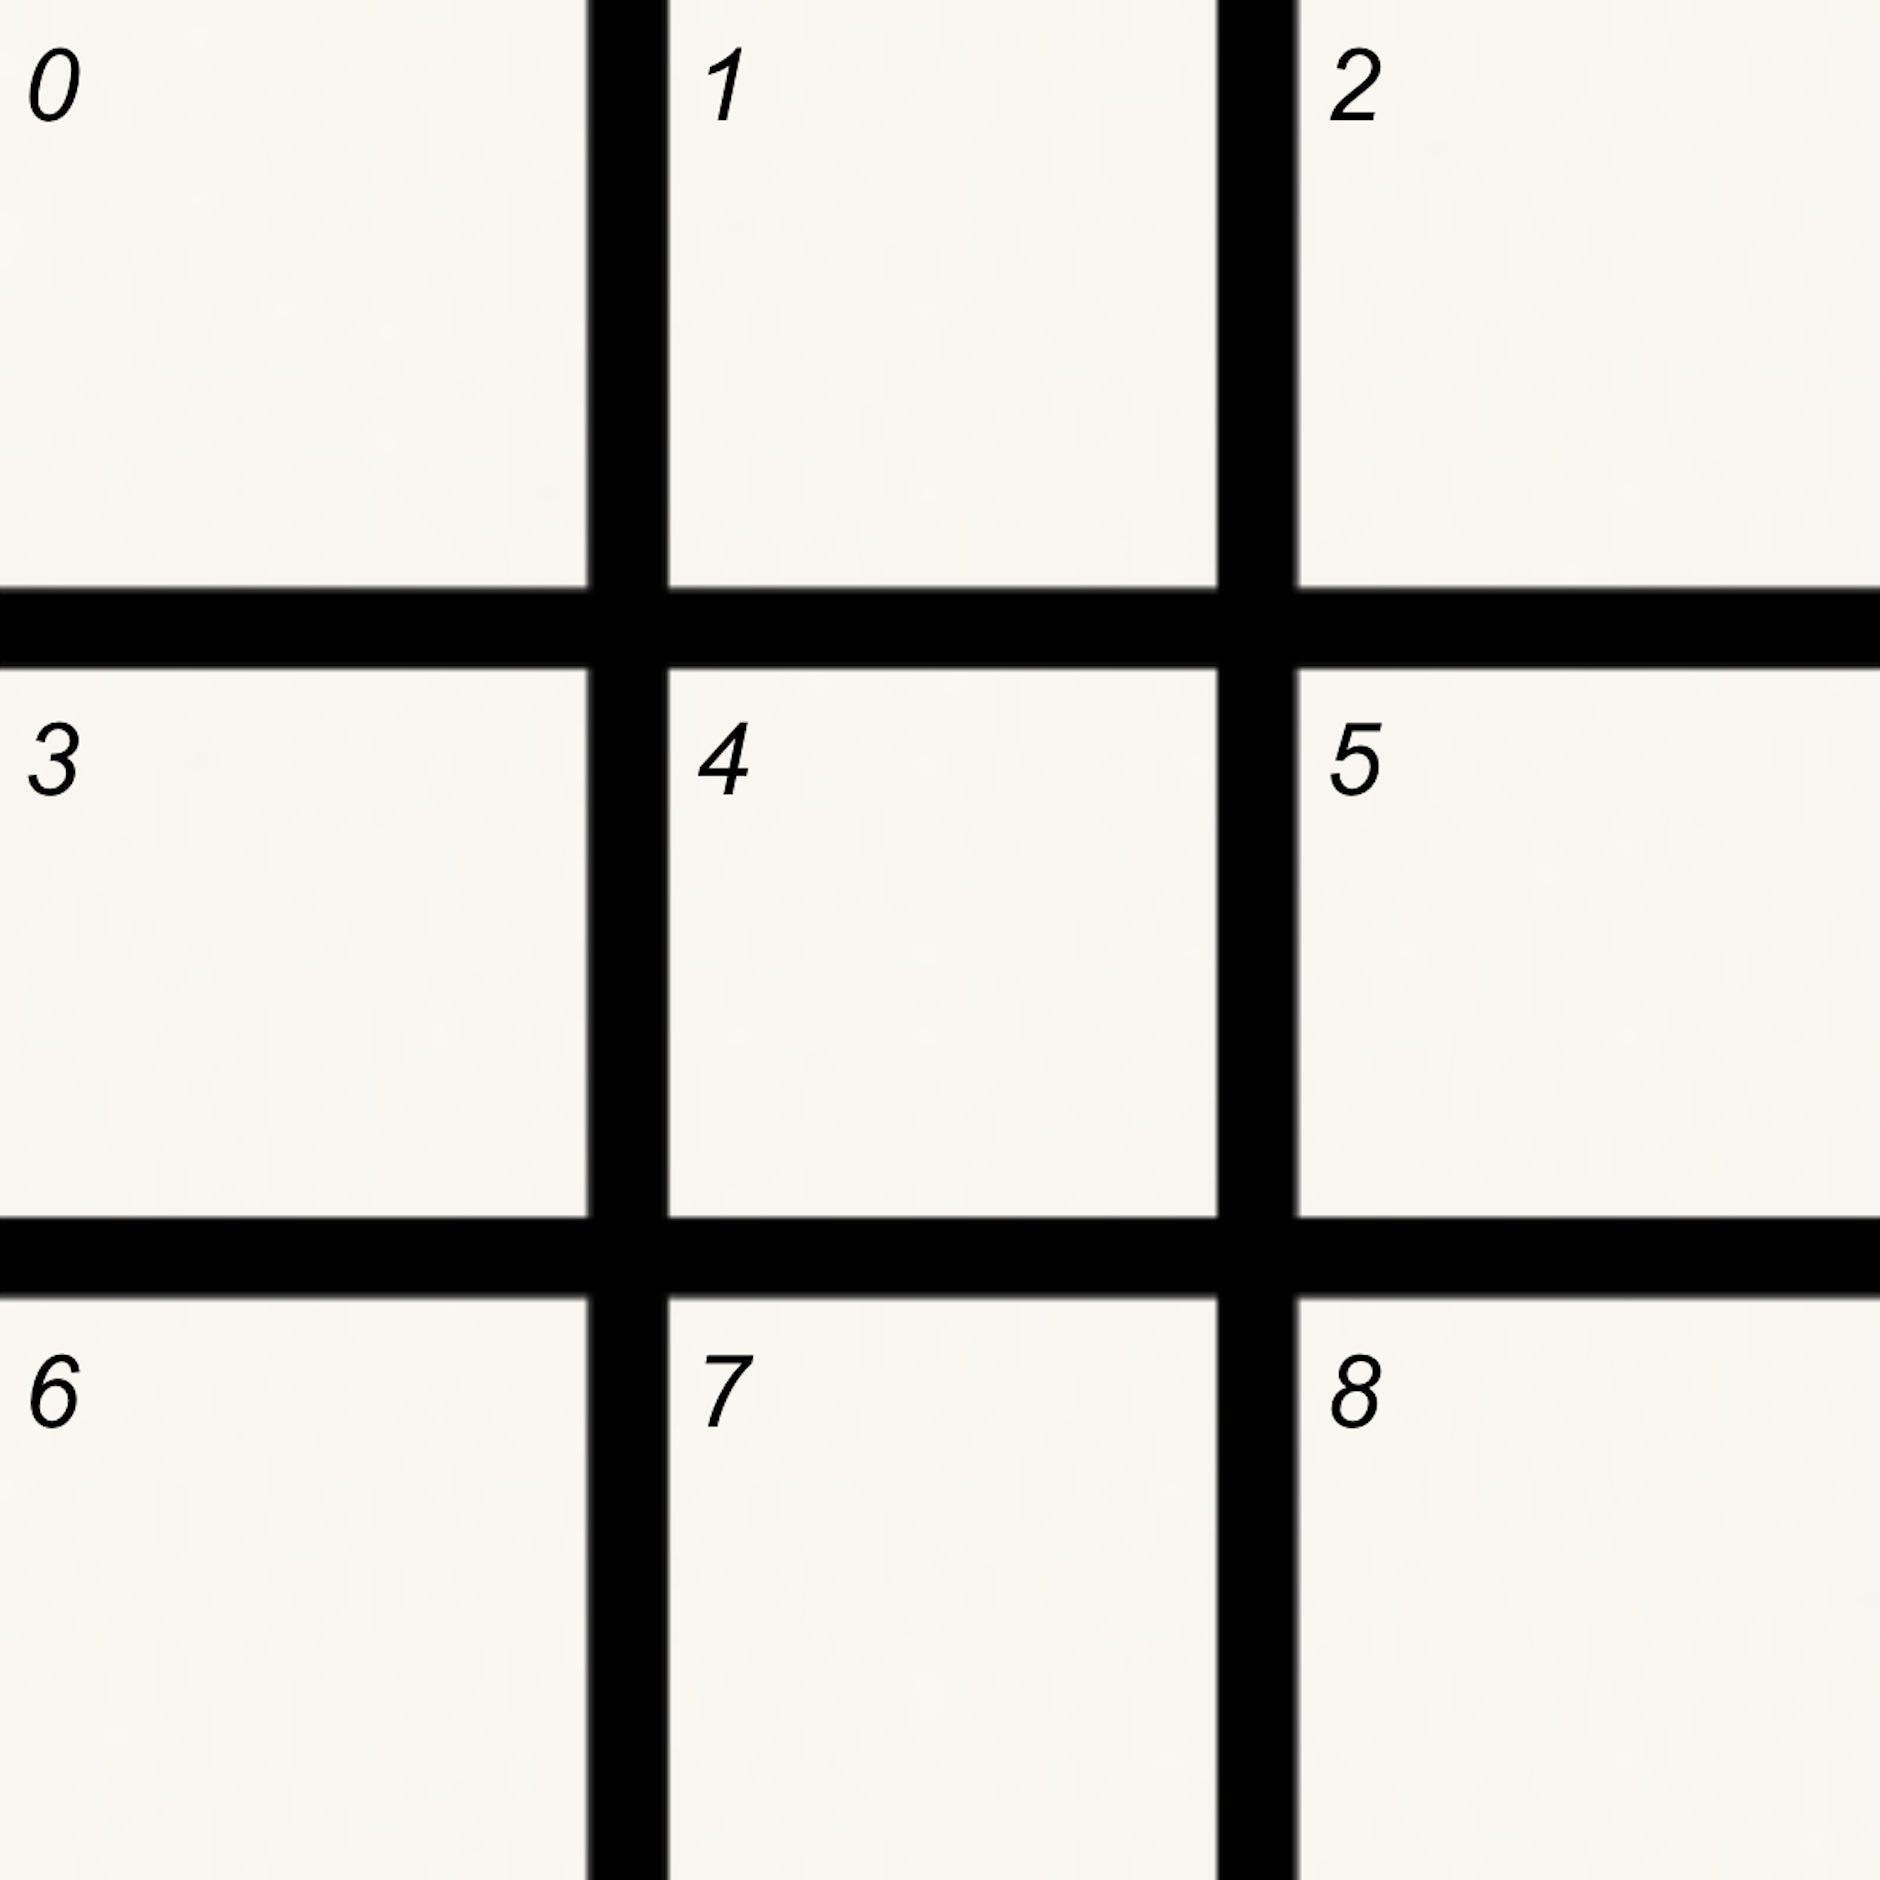
\includegraphics[width=0.5\textwidth, keepaspectratio]{inserted_images/empty_board_fix.png}
\end{center}

In addition to the nine board positions, we introduce two special
tokens:

\begin{itemize}
\tightlist
\item
  \texttt{9} is a start token, placed at the beginning of every game.
\item
  \texttt{10} is a padding token, used to pad the game sequence once
  the game is over but the board isn't yet full. Padding allows us to ensure
  that every game sequence has the same fixed length for training.
\end{itemize}

With these eleven tokens, we can represent every game of tic-tac-toe as
a list of 10 tokens. Importantly, the tokens don't specify which players
made each move. As humans who know the rules of the game, we know that
Player A and Player B alternate moves, but the model sees only the
sequence of moves, and must implicitly learn this alternation structure
during training.

Let's go over an example to clarify. Every game starts with a sequence
of \texttt{{[}9{]}}, and the board looks like the empty board we saw
earlier:

\begin{center}
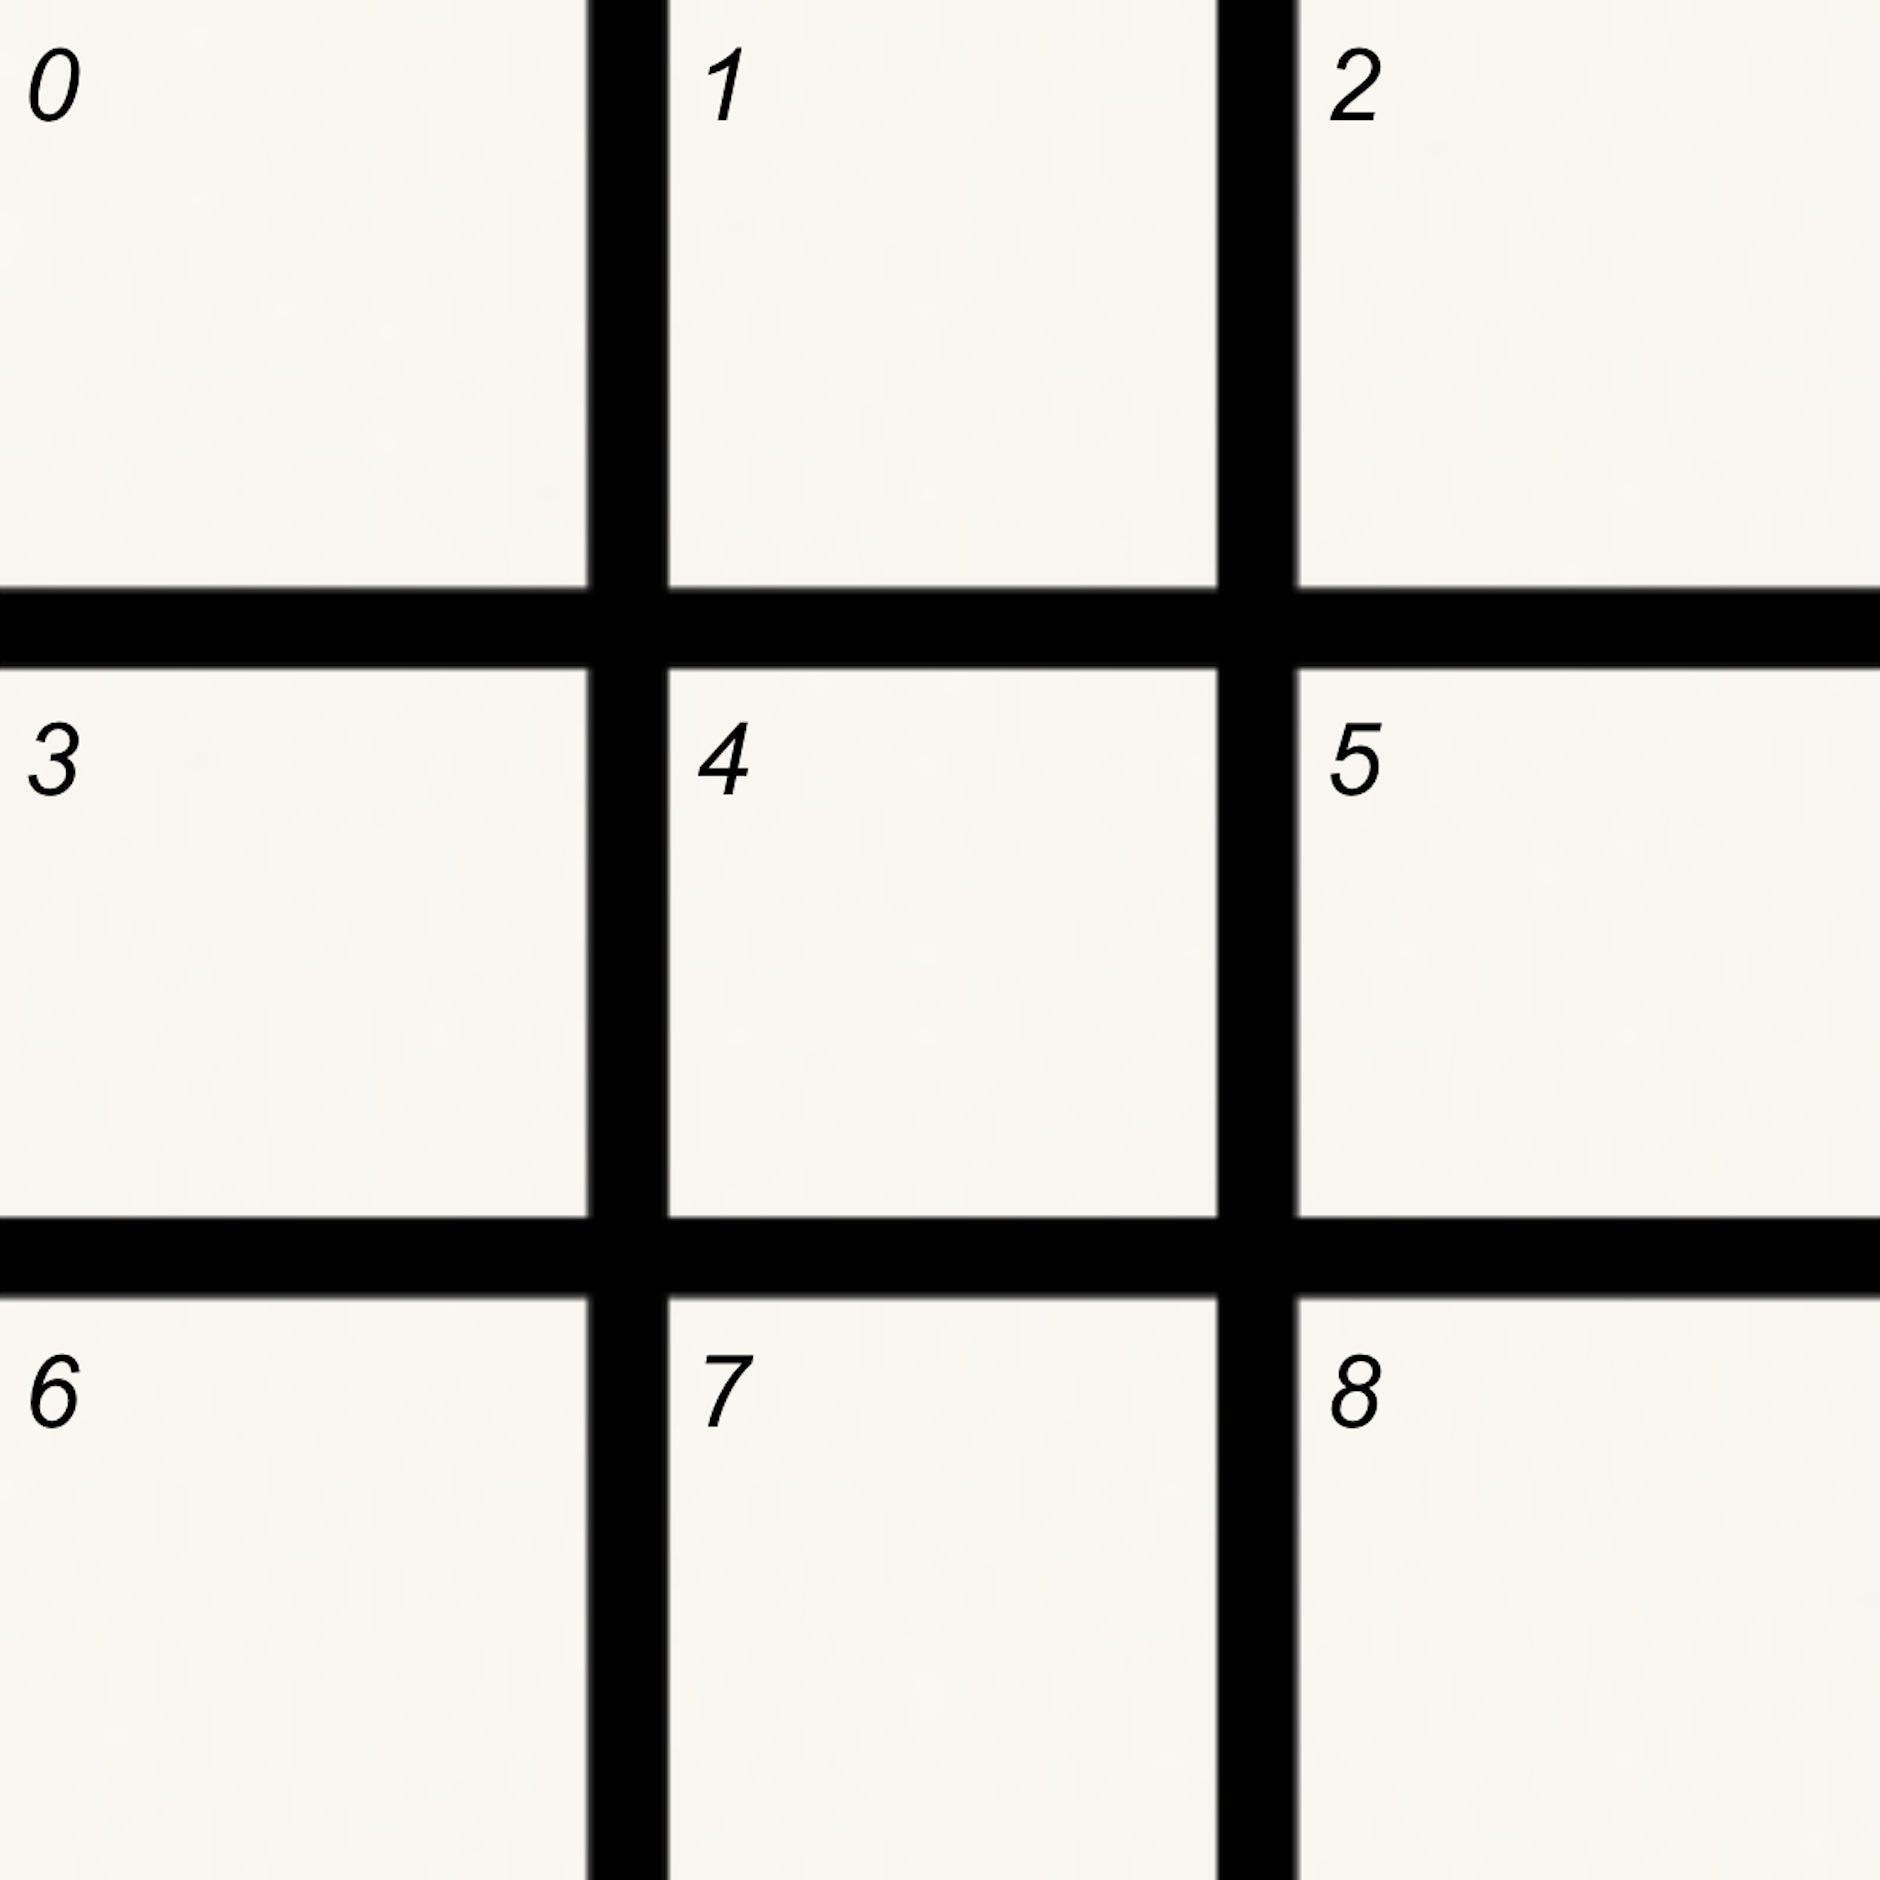
\includegraphics[width=0.5\textwidth]{inserted_images/empty_board_fix.png}
\end{center}

Then, after a few moves have been played, yielding a sequence of
\texttt{{[}9,\ 6,\ 4,\ 2,\ 8,\ 0{]}}, we have a board like this:

\begin{center}
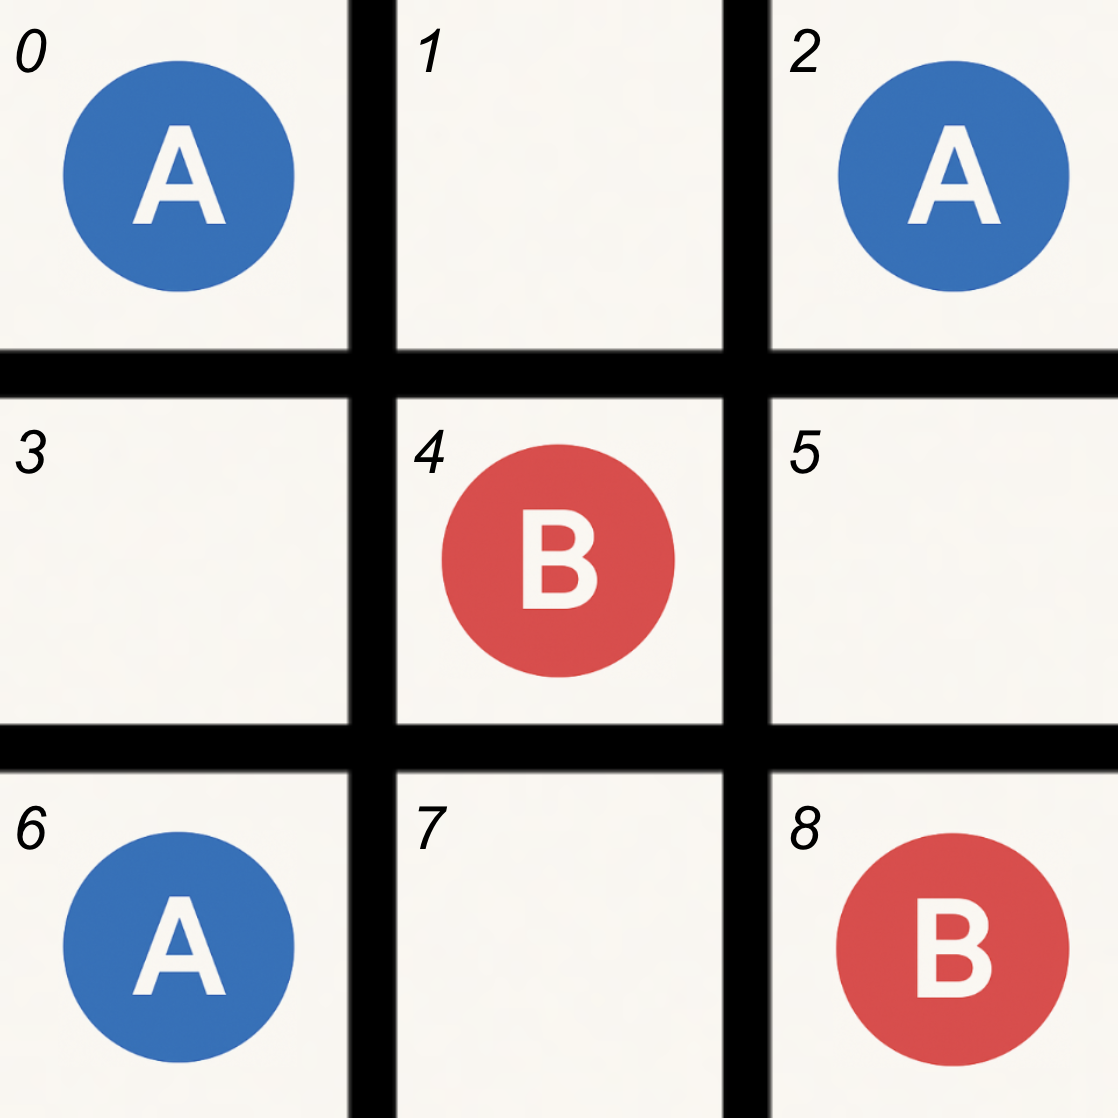
\includegraphics[width=0.5\textwidth,keepaspectratio]{inserted_images/half_game.png}
\end{center}

And finally, when the game ends before the board is full, the rest of
the sequence is filled with padding tokens. For example, finishing the
game above gives the sequence
\texttt{{[}9,\ 6,\ 4,\ 2,\ 8,\ 0,\ 3,\ 1,\ 10,\ 10{]}} and this board:

\begin{center}
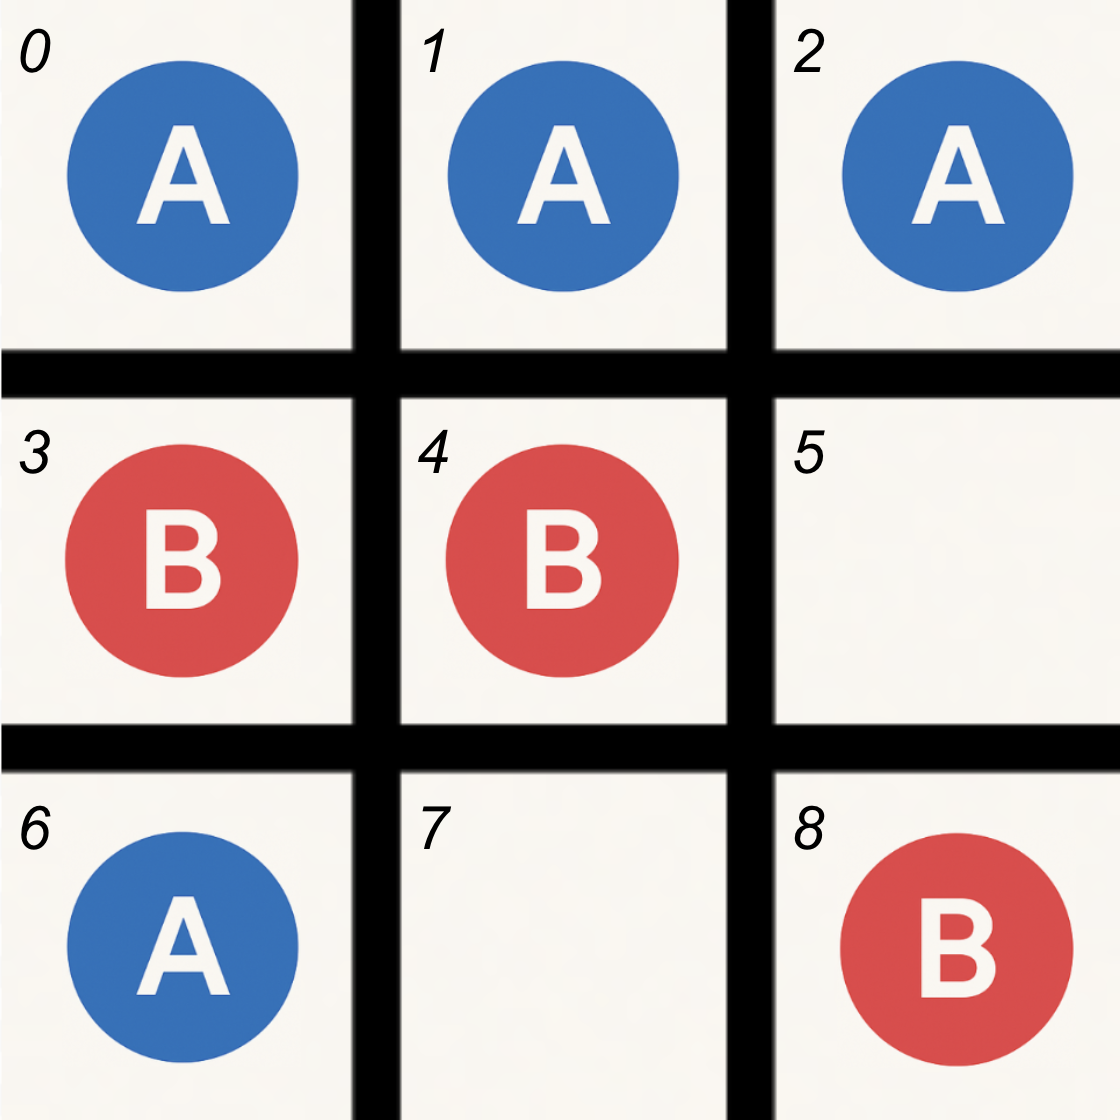
\includegraphics[width=0.5\textwidth,keepaspectratio]{inserted_images/finished_game.png}
\end{center}

Notice how the sequence length of the completed game is 10, even though
the board isn't full? That's because Player A won early, and we used
padding tokens to ensure the game sequence was the correct length.

    \subsection{Generation of example
games}\label{generation-of-example-games}

To produce examples of games that our GPT could train and test on, we
followed the following procedure to build tokenized games:

\begin{equation*}
\begin{aligned}
&\texttt{Initialize:} \\
&\quad \texttt{game} \leftarrow [9] \quad \text{(the start token)} \\
&\quad \texttt{valid\_moves} \leftarrow \{0, 1, 2, 3, 4, 5, 6, 7, 8\} \\
\\
&\texttt{While the game is not over:} \\
&\quad \texttt{move} \leftarrow \text{random choice from valid\_moves} \\
&\quad \texttt{game.append(move)} \\
&\quad \texttt{valid\_moves.remove(move)} \\
&\quad \text{Check if there is a winner or the board is full and break loop if so} \\
\\
&\texttt{Pad the game to length 10:} \\
&\quad \texttt{While len(game) < 10:} \\
&\quad\quad \texttt{game.append(10)} \quad \text{(the padding token)}
\end{aligned}
\end{equation*}

This results in games between players who play without strategy but
always play a valid move. This behavior of randomly selecting a valid
move is what we want our GPT to learn.

    \subsection{Model Architecture}\label{model-architecture}

Our model is based on Karpathy's NanoGPT, whose architecture is as
follows:

\begin{itemize}
\item
  An embedding layer, which includes token embeddings (a unique vector
  learned for each token in the vocabulary) and positional embeddings (a
  unique vector learned for each position in the input sequence). These
  two vectors are summed at each position to embed the input sequence
  into a higher-dimensional space.
\item
  A stack of \href{https://arxiv.org/abs/1706.03762}{Transformer blocks}, each composed of:

  \begin{itemize}
  \tightlist
  \item
    A LayerNorm, which normalizes the input to stabilize training and
    improve optimization.
  \item
    A causal self-attention mechanism, which allows each token to attend
    to earlier tokens in the sequence. This helps the model learn and
    capture interactions between different elements in the sequence.
  \item
    A multi-layer perceptron (MLP), which is a feedforward neural
    network that introduces additional nonlinearity to the outputs of
    the self-attention layer.
  \item
    A residual connection after both the attention and MLP sublayers
    that adds the input to each sublayer back to its output. This helps
    preserve information across layers and makes learning easier by
    allowing the model to make incremental updates rather than
    relearning everything from scratch.
  \end{itemize}
\item
  A final LayerNorm, followed by a linear layer that maps the final
  hidden states to a probability distribution over our tokens for
  next-token prediction.
\end{itemize}

For a more precise and technical idea of how the model works, check out
the GPT Math section of the appendix.

When initializing a GPT, the following parameters can be adjusted:

\begin{itemize}
\tightlist
\item
  \texttt{n\_embd}, the embedding dimension of the embedding layer
\item
  \texttt{n\_head}, the number of attention heads in the self-attention
  mechanism. This must be a factor of \texttt{n\_embd}
\item
  \texttt{n\_layer}, the number of transformer blocks in the model
\end{itemize}

We found that the architecture that Haeusler presented (12-dimensional
embeddings, 1 attention head, and 1 transformer layer) was the simplest
architecture that was able to learn how to play. This architecture is
what is used throughout this project unless stated otherwise.

    \subsection{Training the Model}\label{training-the-model}

How do we train the model? Our GPT is initialized with random weights,
but the goal of training is to update these weights so that the model's
outputs are as accurate as possible, given the input sequence.

We've generated a dataset of full games, each represented as a sequence
of 10 tokens. However, we want the model to learn to make predictions
after any number of moves, not just at the end of the game. So we split
each game into many training examples.

For example, say we have the full game
\texttt{{[}9,\ 6,\ 4,\ 2,\ 8,\ 0,\ 3,\ 1,\ 10,\ 10{]}} in our training
dataset. We can generate multiple prediction tasks from this:

\begin{itemize}
\tightlist
\item
  From \texttt{{[}9{]}}, predict \texttt{6}
\item
  From \texttt{{[}9,\ 6,\ 4{]}}, predict \texttt{2}
\item
  From \texttt{{[}9,\ 6,\ 4,\ 2,\ 8,\ 0,\ 3,\ 1{]}}, predict \texttt{10}
\end{itemize}

The ground truth is always the next token in the sequence. The model is
trained by passing in these input sequences, where it predicts
probabilities\footnote{Actually, the model outputs logits, which can then be
converted to probabilities. I find it easier to think about
probabilities than logits, so we'll pretend these are probabilities.
The conversion from logits to probabilities is very simple.} for the next token given the input sequence. We
compute how accurate its output predictions are and then update the
weights to improve performance. We quantify how accurate the model's
predictions are by using a loss function called cross-entropy loss,
which is calculated as follows:

Let \(p = (p_0, p_1, \dots, p_{n})\) be the model's predicted
probability distribution over n tokens.\\
Let \(y \in \{0, 1, \dots, n\}\) be the index of the correct (target)
token.

Then the cross-entropy loss is:

\[
\mathcal{L} = -\log(p_y)
\]

This loss is small when the model assigns high probability to the
correct token, and large when it assigns low probability to the correct
token.

We take the average of the loss function over a batch of examples and
use this overall loss to change the model. Then, we use backpropagation
to compute the gradient of the loss with respect to each parameter, and
use an optimizer to adjust the weights in a direction that reduces the
loss. This model uses the AdamW optimizer, which is a slight
modification of gradient descent that typically leads to faster and more
stable convergence. Unless stated otherwise, we trained the model for
100,000 iterations, where an iteration is defined as one update of the
model's weights. Finally, once training is done, we evaluate the model
for a final time on an unseen validation dataset.

Here's some pseudocode showing how the training loop works:

\begin{equation*}
\begin{aligned}
&\texttt{Initialize:} \\
&\quad \texttt{model} \leftarrow \text{randomly initialized GPT} \\
&\quad \texttt{optimizer} \leftarrow \text{AdamW optimizer} \\
&\quad \texttt{iter} \leftarrow 0 \\
\\
&\texttt{Repeat for 100,000 iterations:} \\
&\quad \texttt{X, Y} \leftarrow \text{sample a batch of training examples} \\
&\quad \texttt{logits} \leftarrow \texttt{model.forward(X)} \\
&\quad \texttt{loss} \leftarrow \text{cross-entropy between logits and Y} \\
&\quad \texttt{compute gradients of loss} \\
&\quad \texttt{update model weights using optimizer} \\
&\quad \texttt{iter} \leftarrow \texttt{iter + 1} \\
\\
&\texttt{After training:} \\
&\quad \texttt{evaluate model on validation set}
\end{aligned}
\end{equation*}

    \section{Answering our Research
Questions}\label{answering-our-research-questions}

\subsection{Model Success}\label{model-success}

First, let's confirm that the model is able to play legal games of
tic-tac-toe. We trained 100 versions of the same model, and among those
that finished training within the given training time, they generated
valid games 99.1\% of the time. \emph{How} does this model learn? Well,
that's what we'll discuss in the rest of this document.

    \subsection{Model Originality}\label{model-originality}

The trained model can successfully play a game of tic-tac-toe. But how
does it do that? Might it just be memorizing the games we showed it as
it trained, and repeating them back exactly? This would be bad,
especially when we think about what it would mean for large language
models: what if ChatGPT could only regurgitate exact writing that it had
seen before? These models are only useful if they can generate novel
games (or text), so we test this capability.

To test the model's creativity, we train the model on 100,000
synthetically generated games of tic-tac-toe. These games are
created by randomly choosing a move for players until one player wins or
the board is filled. After training, we have the model generate 1,000
games and measure how many of them appeared in the training set. Across
100 training trials (62 of which learned to play successfully before
100k iterations, which we'll call the models that ``converged'' later
on), the mean originality score was 58.1\%.

\[
\text{Originality Score} = 1 - \frac{\text{\# of generated games present in training dataset}}{\text{total \# of games generated}} = 1 - \frac{419}{\text{1000}} = 58.1\%
\]

Next, we consider what kind of originality score we should expect. Since
there are 255,168 possible games of Tic-Tac-Toe and our synthetic
dataset includes 100,000 of them, we'd expect the model's originality to
reflect the proportion of games not seen during training:\footnote{We would actually expect an originality score slightly
higher than 60.8\%, because the synthetic games are randomly generated,
and can include overlapping games. A dataset with 100,000 elements is
highly unlikely to have 100,000 distinct elements, but this is an
expected floor for our originality score.}

\[
\frac{255,\!168 - 100,\!000}{255,\!168} \approx 60.8\%
\]

    So, the model is able to generate unseen game sequences at approximately
the rate we'd expect.\footnote{This value is slightly smaller than the rate we'd expect. I
think this is happening because some of the 255,168 games are more
likely to occur when creating the synthetic dataset. For example, to
match a short game when Player A wins quickly, only five moves need to
match, but to match a long game, nine moves need to match. This means
the short games are more likely to be generated synthetically (and be in
our training data), and are more likely to be generated by any model
that selects between moves randomly. This should drive originality
scores down. To test this hypothesis, I generated a new dataset of games
as described before, effectively simulating a model that chooses valid
moves at random. I then treated these as if they were model-generated
games and calculated their originality score relative to the original
training set. The resulting originality score was 58.8\%, nearly
identical to the GPT's. This supports the idea that lower originality
scores than expected are a natural consequence of the data distribution,
rather than evidence of any memorization.} It is not memorizing, but instead seems
to be learning the rules of the game and generating games it has never
seen before. We'll explore how it does that in the following section.

    \subsection{Learning the Rules of the
Game}\label{learning-the-rules-of-the-game}

What are the rules of tic-tac-toe? Without thinking about any strategy,
we can define two things a player needs to do in order to play by the
rules:

\begin{enumerate}
\def\labelenumi{\arabic{enumi}.}
\item
  Pick a space that neither player has played in before to place their
  piece. A space can't be occupied by multiple pieces, and if a player
  tries to play on top of another piece, a mistake has been made.
\item
  A player wins by placing three of their pieces consecutively in any
  row, column, or diagonal (we'll call this ``three in a row'' from now
  on, because that is typically how people refer to the game). If the
  game is over and a player tries to play, or the game is not over and a
  player states that it is, a mistake has been made.
\end{enumerate}

\textbf{Keep these rules in mind!} They'll be very important for the
rest of this document.

Let's take a closer look at the 62 training trials that learned to play
successfully to see how these models might be learning the two rules
stated above. Plotted below is the validation loss by iteration for each
of the trials. The graph is a little messy since there are so many
trials shown, but take a look and see if you notice a trend:

\begin{center}
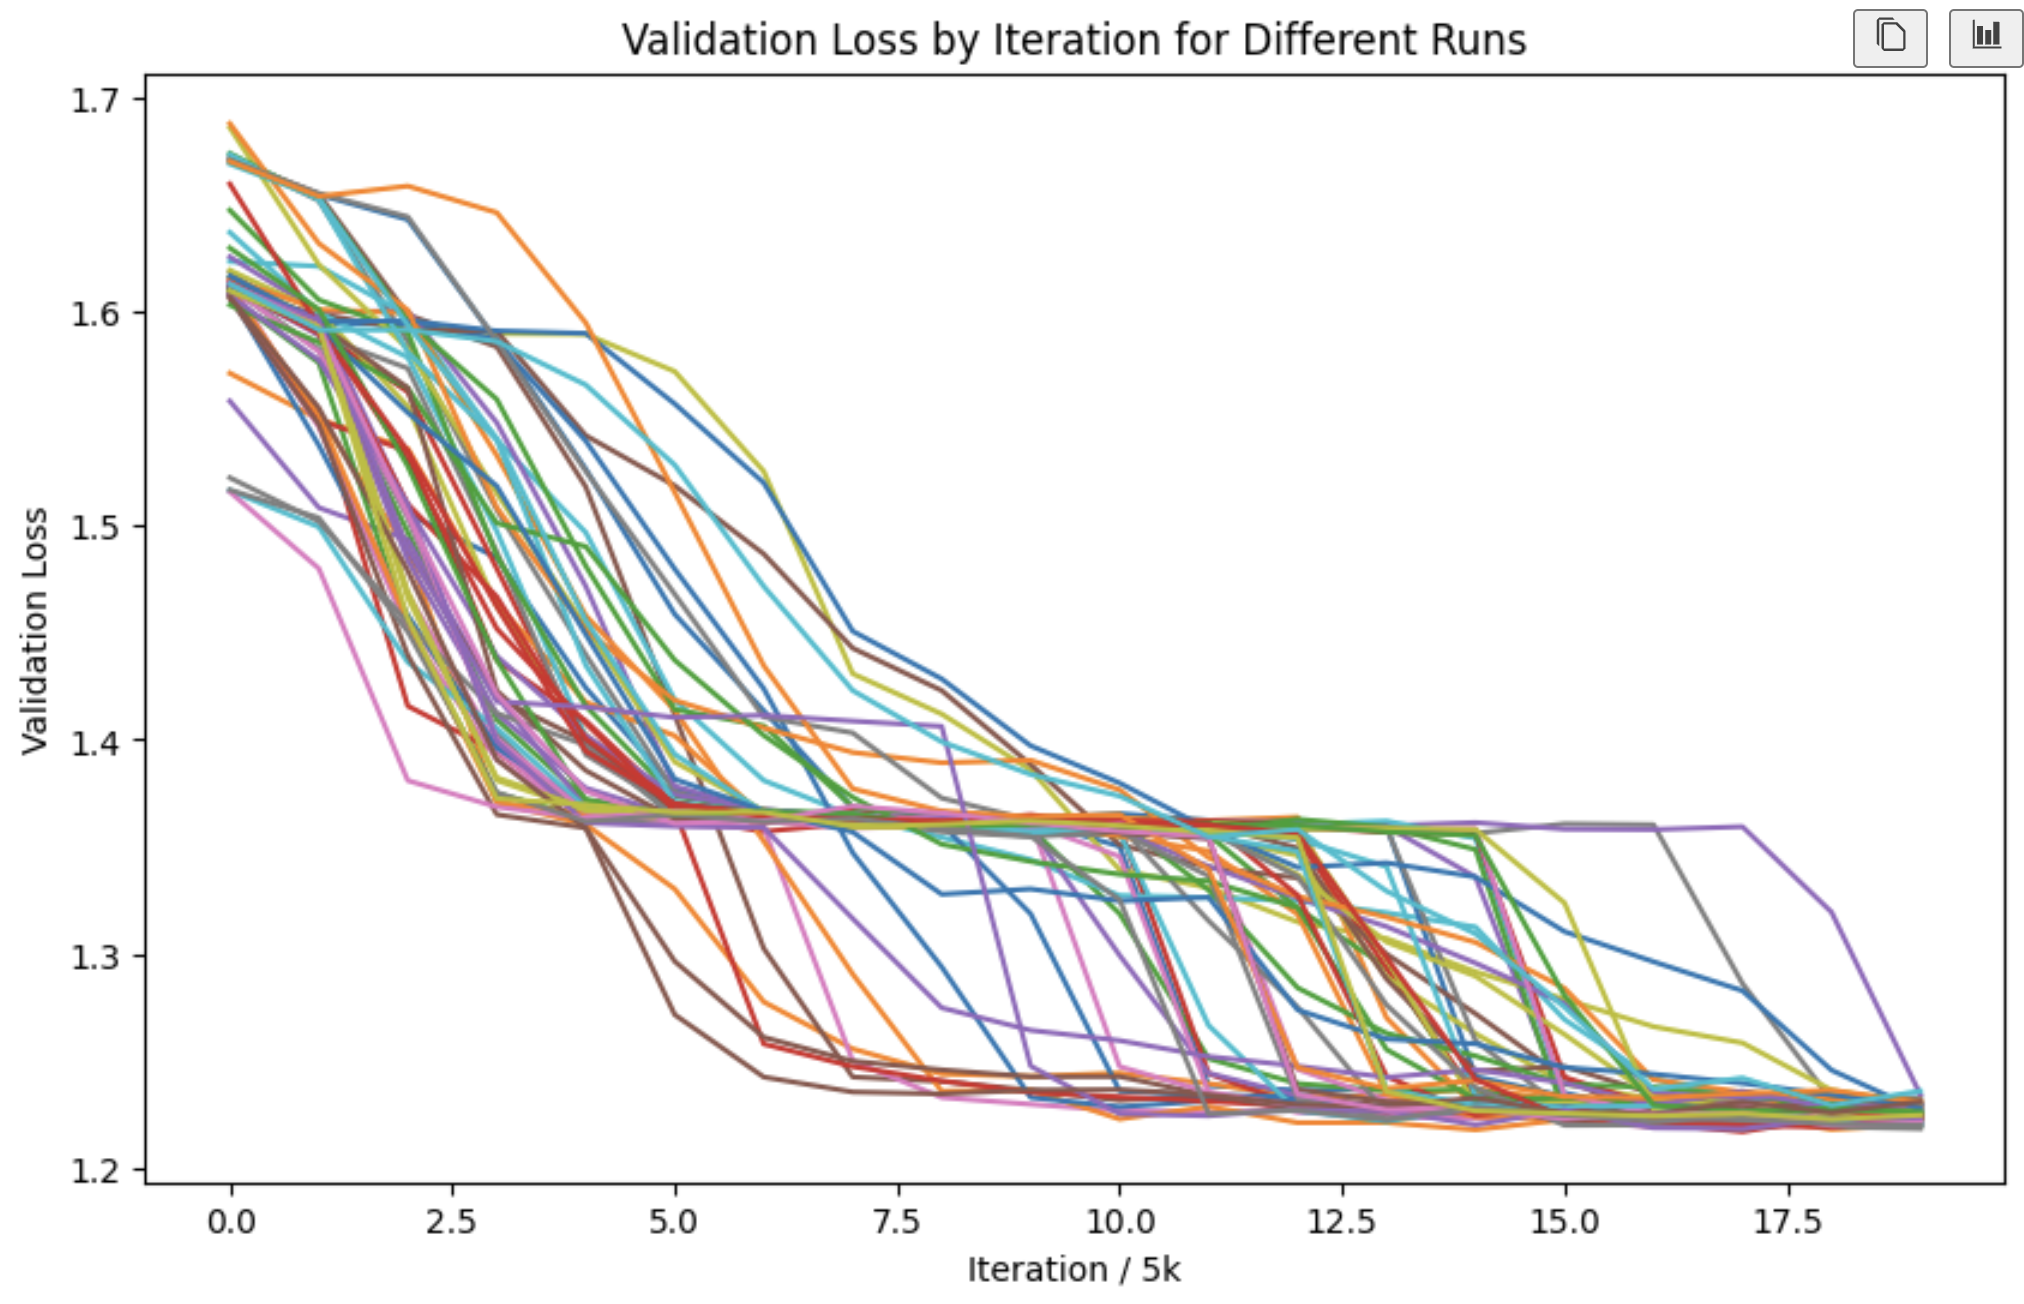
\includegraphics[keepaspectratio]{inserted_images/converging_runs.png}
\end{center}

    Notice how many trials stall with a validation loss between 1.36 and
1.37? In fact, \textgreater70\% of the runs that converge exhibit this
stalling behavior for at least 5,000 iterations. Let's take a closer
look at them and see what's going on\ldots{}

We'll define two new statistics to measure how well a model understands
the rules: 1. Invalid Move Rate: This measures how often the model
generates a move that has been previously played in the game sequence.
It is computed over all generated games (rather than all generated
moves), so if a game has any invalid move, it is counted towards the
invalid rate. It is calculated as follows:

\[
\text{Invalid Move Rate} = \frac{\text{\# of generated games with an occupied space generated}}{\text{Total \# of generated games}}
\]

\begin{enumerate}
\def\labelenumi{\arabic{enumi}.}
\setcounter{enumi}{1}
\tightlist
\item
  Correct Ending Rate: This measures how often the model predicts that
  the padding token will be the next token when given a game with a
  winner. In the training data, whenever a game ends before 9 moves
  (meaning a player has won before the board is full), the game sequence
  appends padding tokens to preserve the full sequence length. Once a
  model learns Rule 2, it should always predict the padding token when
  given a game completed before 9 moves have been played to mirror this
  pattern in the training data. It is calculated as follows:
\end{enumerate}

\[
\text{Correct Ending Rate} = \frac{\text{\# of correct padding predictions after an early win}}{\text{\# of generated games resulting in either player winning early}}
\]

Shown below are a few examples of the trials that exhibited this
stalling behavior. Notice the pattern between the validation loss
(rescaled to fit on the same axes), the invalid move rate, and the
correct ending rate.

\begin{center}
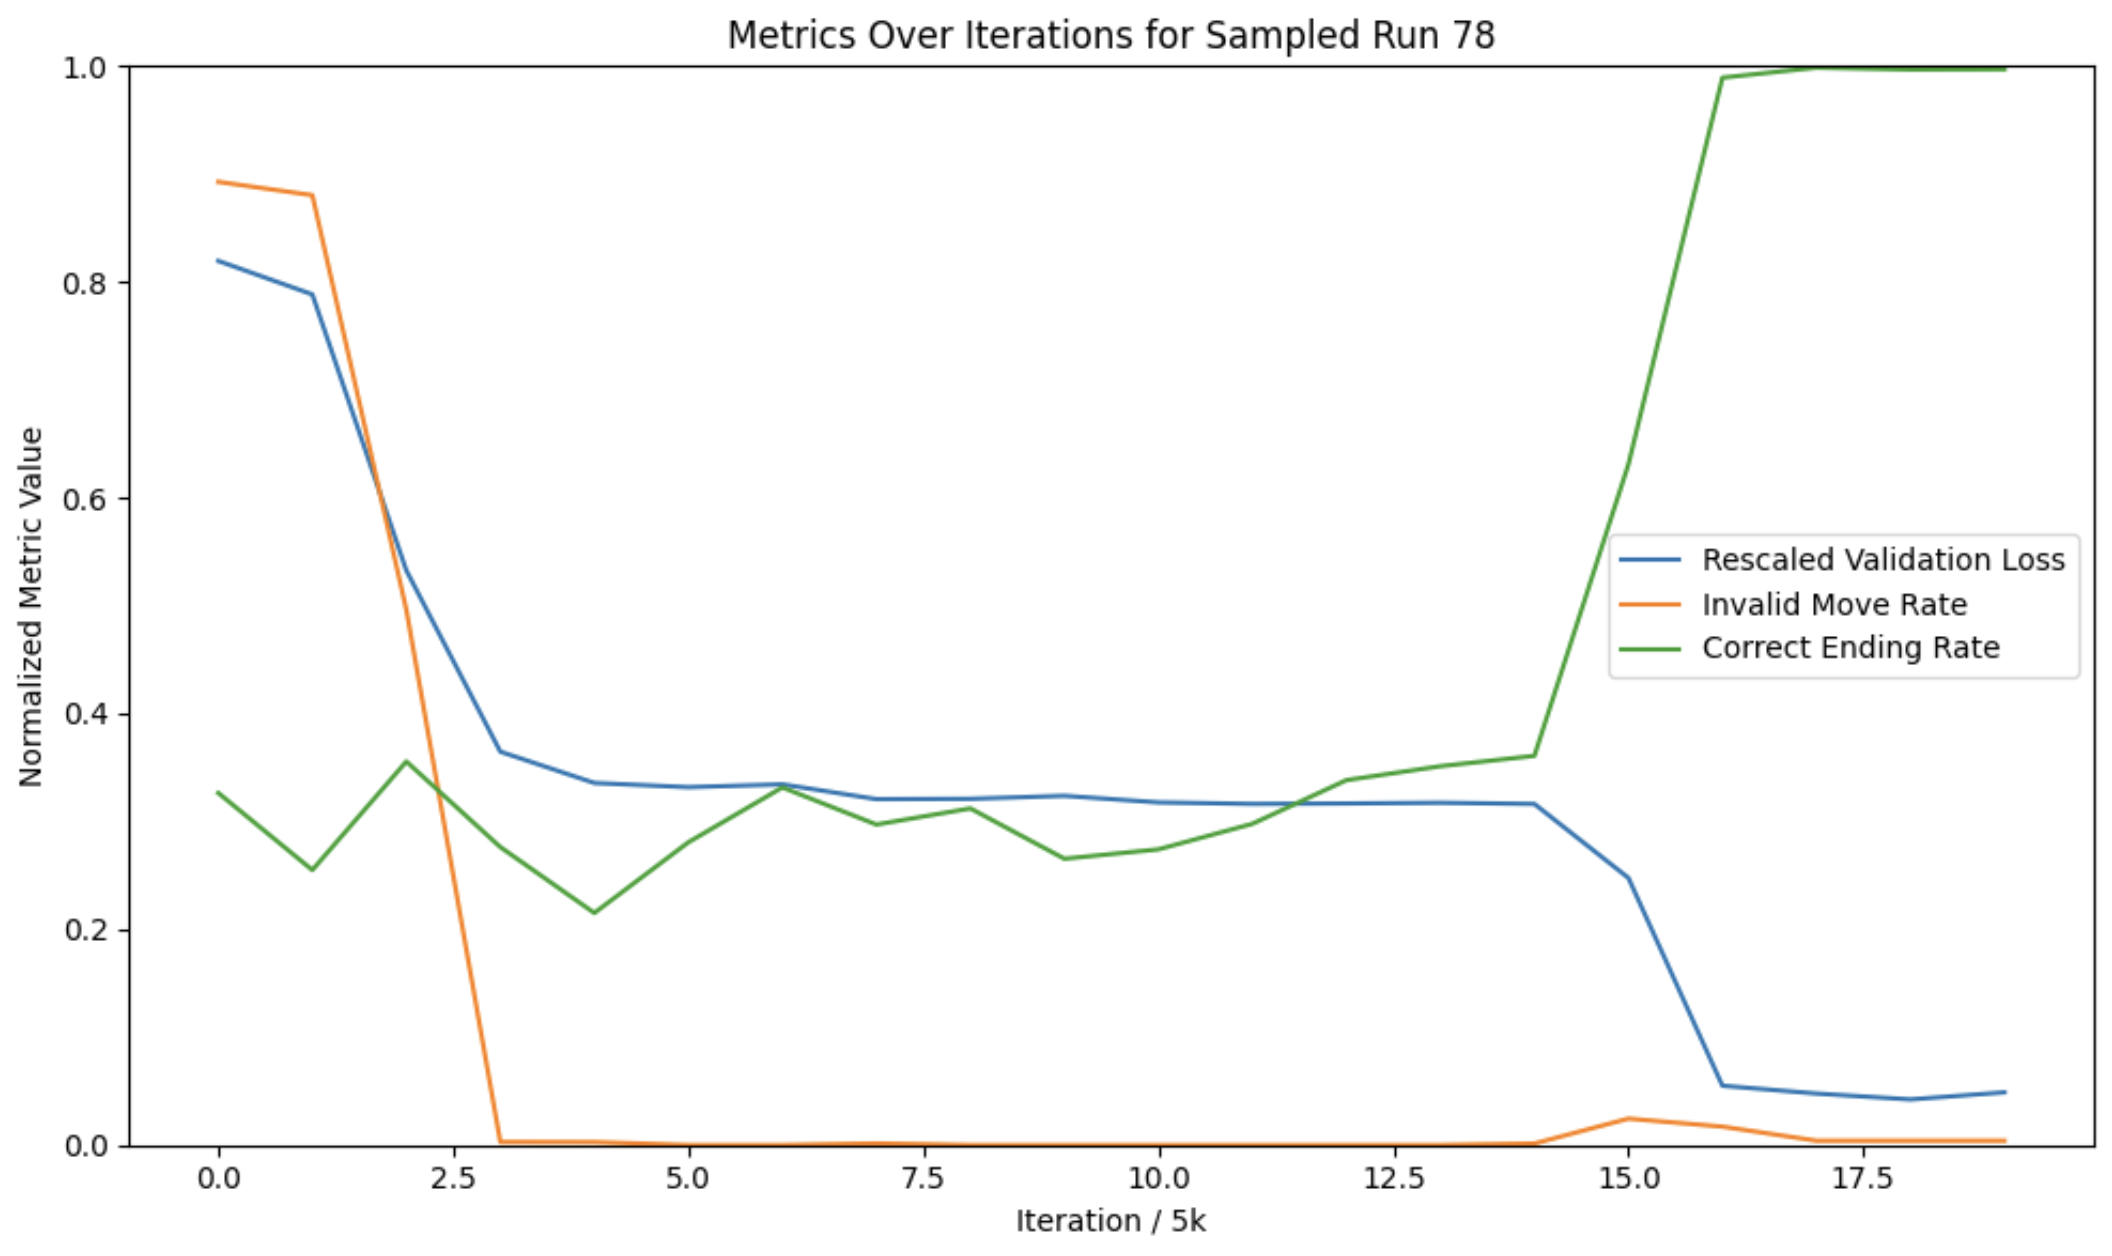
\includegraphics[width=0.67\textwidth,keepaspectratio]{inserted_images/ex1.png}

\vspace{1em} 

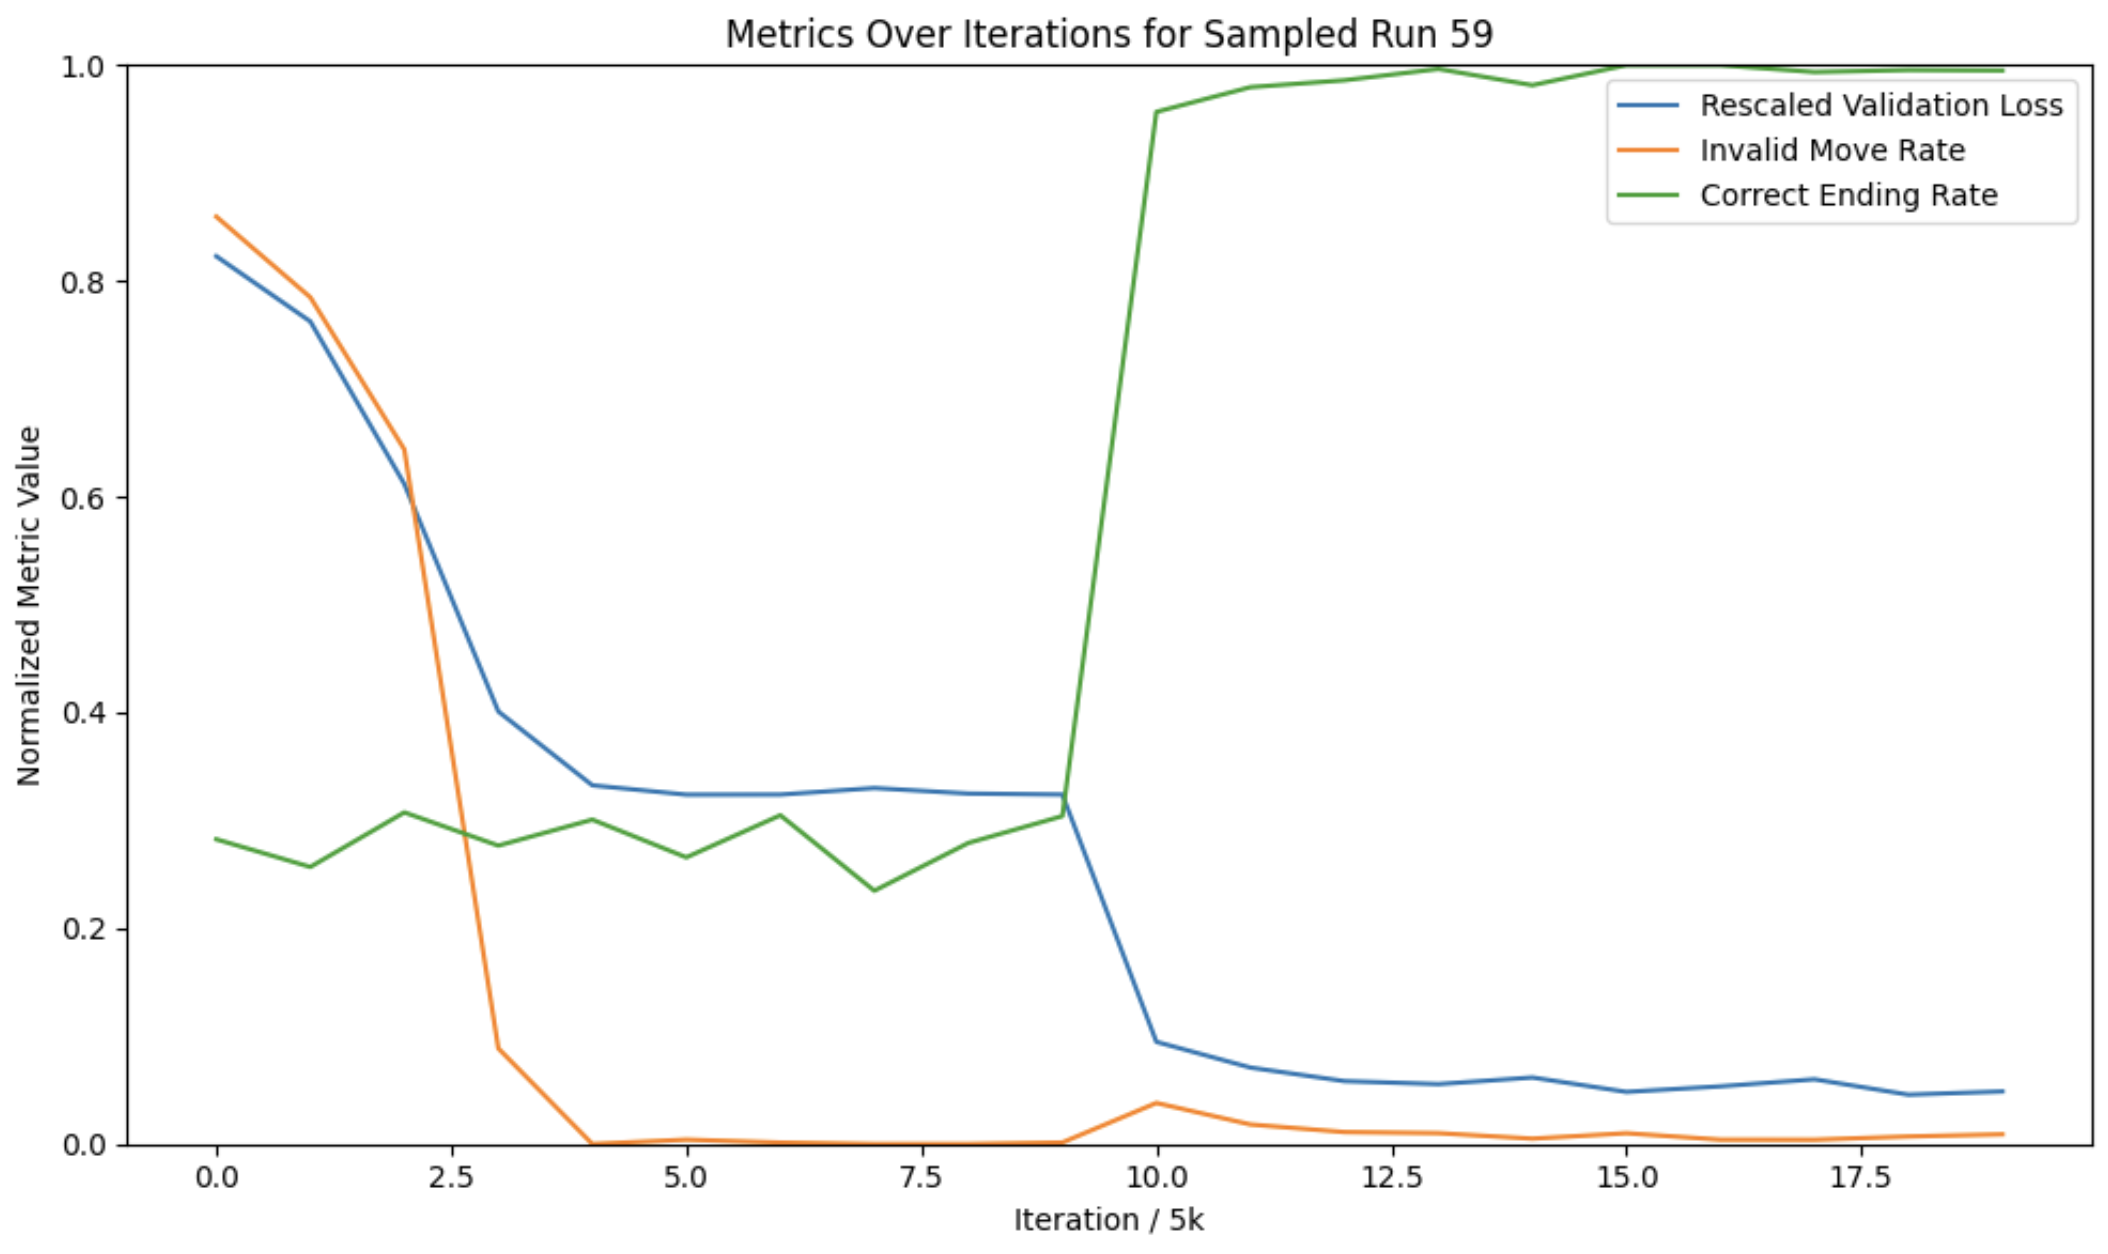
\includegraphics[width=0.67\textwidth,keepaspectratio]{inserted_images/ex2.png}

\vspace{1em}

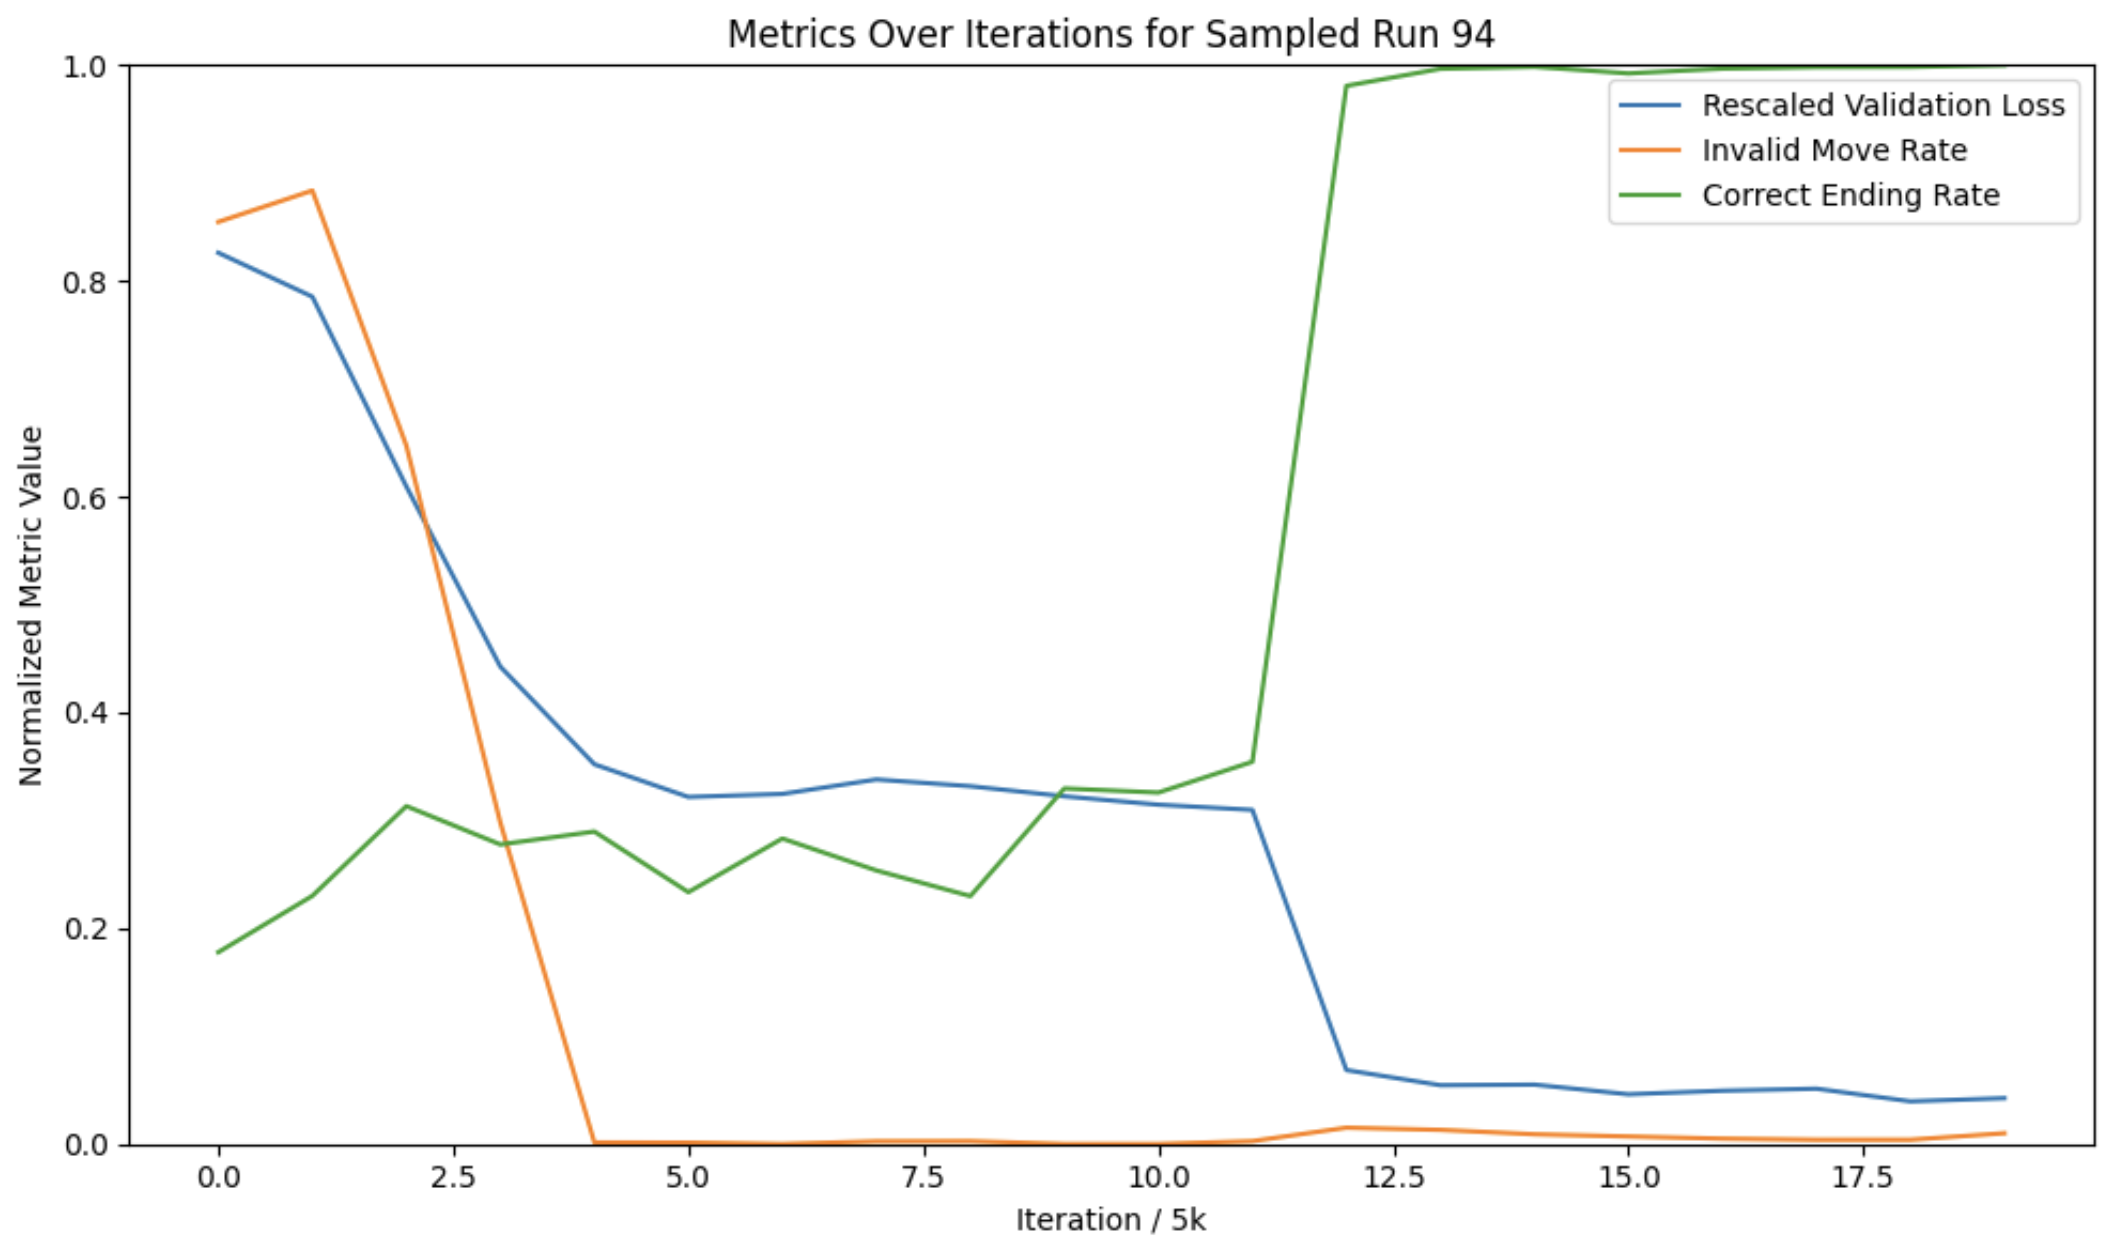
\includegraphics[width=0.67\textwidth,keepaspectratio]{inserted_images/ex3.png}
\end{center}

    The first thing to note is that, in all of these trials, the correct
ending rate approaches 1 and the invalid move rate approaches 0 by the
end of training. This means that by the end of training, the model
successfully learns the rules of tic-tac-toe! It can avoid playing in
occupied spaces and identifies when the game has been won.

Next, observe that the validation loss drops in two stages. During the
first one, the invalid move rate drops nearly to 0, but the correct
ending rate stagnates and/or fluctuates randomly, showing no
improvement. Then, during the second drop, the invalid move rate
increases slightly while the correct ending rate drastically increases.
As training finishes, the correct ending rate gets even higher, and the
invalid move rate slowly decreases back towards 0. This trend holds for
all of the trials that stall with a loss between 1.36 and 1.37 for at
least 5,000 iterations. Keep hitting play on the cell above to randomly
select more trials and confirm this trend.

Clearly, the model seems to be learning the two rules of tic-tac-toe
separately, first learning to play in unoccupied spaces and next
learning to identify winners, but what is going on internally when this
happens? \emph{How} does this learning occur?

    \subsection{Internal Game
Representation}\label{internal-game-representation}

\subsubsection{Background Work}\label{background-work}

A \href{https://arxiv.org/abs/2210.13382}{research team from Harvard,
MIT, and Northeastern} created a model called OthelloGPT, which was a
GPT trained to generate games of Othello, another simple board game.
Like our tic-tac-toe GPT, it was able to generate valid moves with very
few errors. This team's central question was whether OthelloGPT had
learned an internal representation of the game state without knowledge
of the rules of the game.

To study this, they drew inspiration from \href{https://arxiv.org/abs/1610.01644}{Alain and Bengio}, who introduced the idea of a \emph{probe}: a model trained to predict some task using a different model's activations. The OthelloGPT team created classifier probes and trained them to predict the state of each space on the board (empty, Player A, or Player B) from the model’s internal activations after being given a sequence of moves. For each layer, they created a dataset by pairing the activations at that layer with the board state implied by the input sequence that produced them. This allowed them to evaluate what information about the board was encoded at different depths of the model.

They compared probes trained on a randomly initialized model with probes
trained on a fully trained model. The tables below show their results.
The Randomized row describes the probe's error rate on the randomly
initialized model, and the Synthetic row describes the probe's error
rate on the fully trained model.\footnote{They also include a Championship row, which comes from
training the model on real games played between skilled players, not
randomly generated games. We can ignore this row.} Each column describes the
error rate of probes trained from different layers of OthelloGPT, with
further right columns corresponding to later layers. Keep in mind for
later that these error rates are not directly comparable to those
produced to our model, as Othello and tic-tac-toe are different games,
and our model has a less complex architecture than OthelloGPT.

Here's their data from the linear probe:

\begin{center}
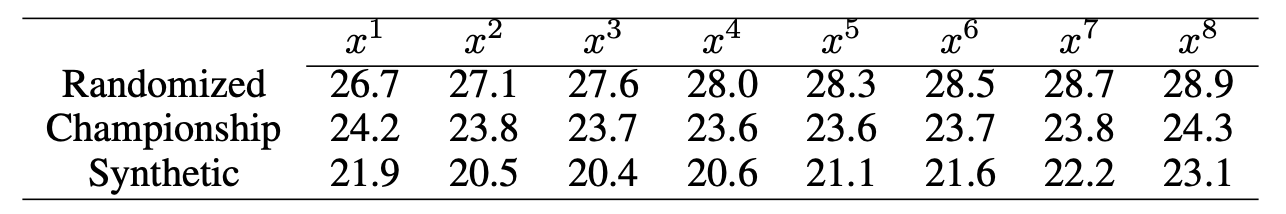
\includegraphics[keepaspectratio]{inserted_images/othello_linear.png}
\end{center}

And here's their data from the MLP probe:

\begin{center}
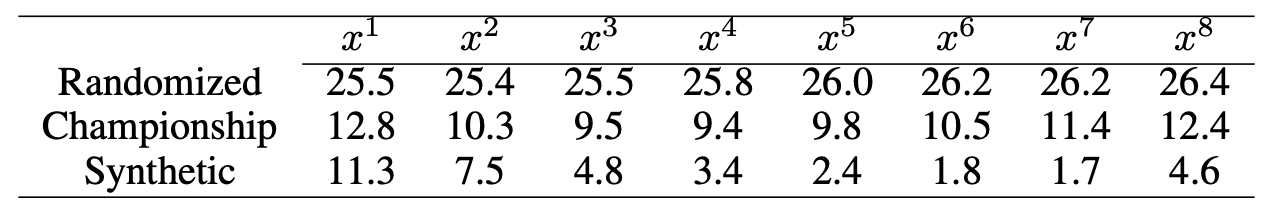
\includegraphics[keepaspectratio]{inserted_images/othello_mlp.png}
\end{center}

On the untrained model, both linear and nonlinear probes performed
poorly, showing that the probes themselves were not powerful enough to
extract board state from random transformations of the input sequence.
On the trained model, however, a nonlinear probe was able to recover the
full board state with up to 98\% accuracy. This is notable because it
shows that during training, OthelloGPT developed an internal
representation of the game state, \emph{even though it was never
explicitly told the rules of the game, and was only asked to predict the
next move}. The linear probe, by contrast, still struggled, performing
only slightly better on the trained model than on the untrained model.
This suggests that the learned representation was nonlinear.

However,
\href{https://www.neelnanda.io/mechanistic-interpretability/othello}{Neel
Nanda} further investigated the internal game representation of
OthelloGPT. Instead of training the probe to classify a space as Player
A/Player B/Empty, he modified the task to classify a space as
``Me''/``You''/Empty from the perspective of the model. If the model is
making a move for a given player, the pieces placed by that player are
``Me'' spaces, and pieces placed by the other player are ``You'' spaces.
With this modified task, he found that a linear probe was able to
reconstruct the board state.

Here's what this other approach looks like for tic-tac-toe: Say we have
input sequence \texttt{{[}9,\ 2,\ 5,\ 3,\ 4,\ 0{]}}. Recall from the
model architecture section that 9 is the start token, and the remaining
tokens indicate where Player A and Player B place their alternating
moves. In a Player A/Player B representation, the board unsurprisingly
looks as follows:

\begin{center}
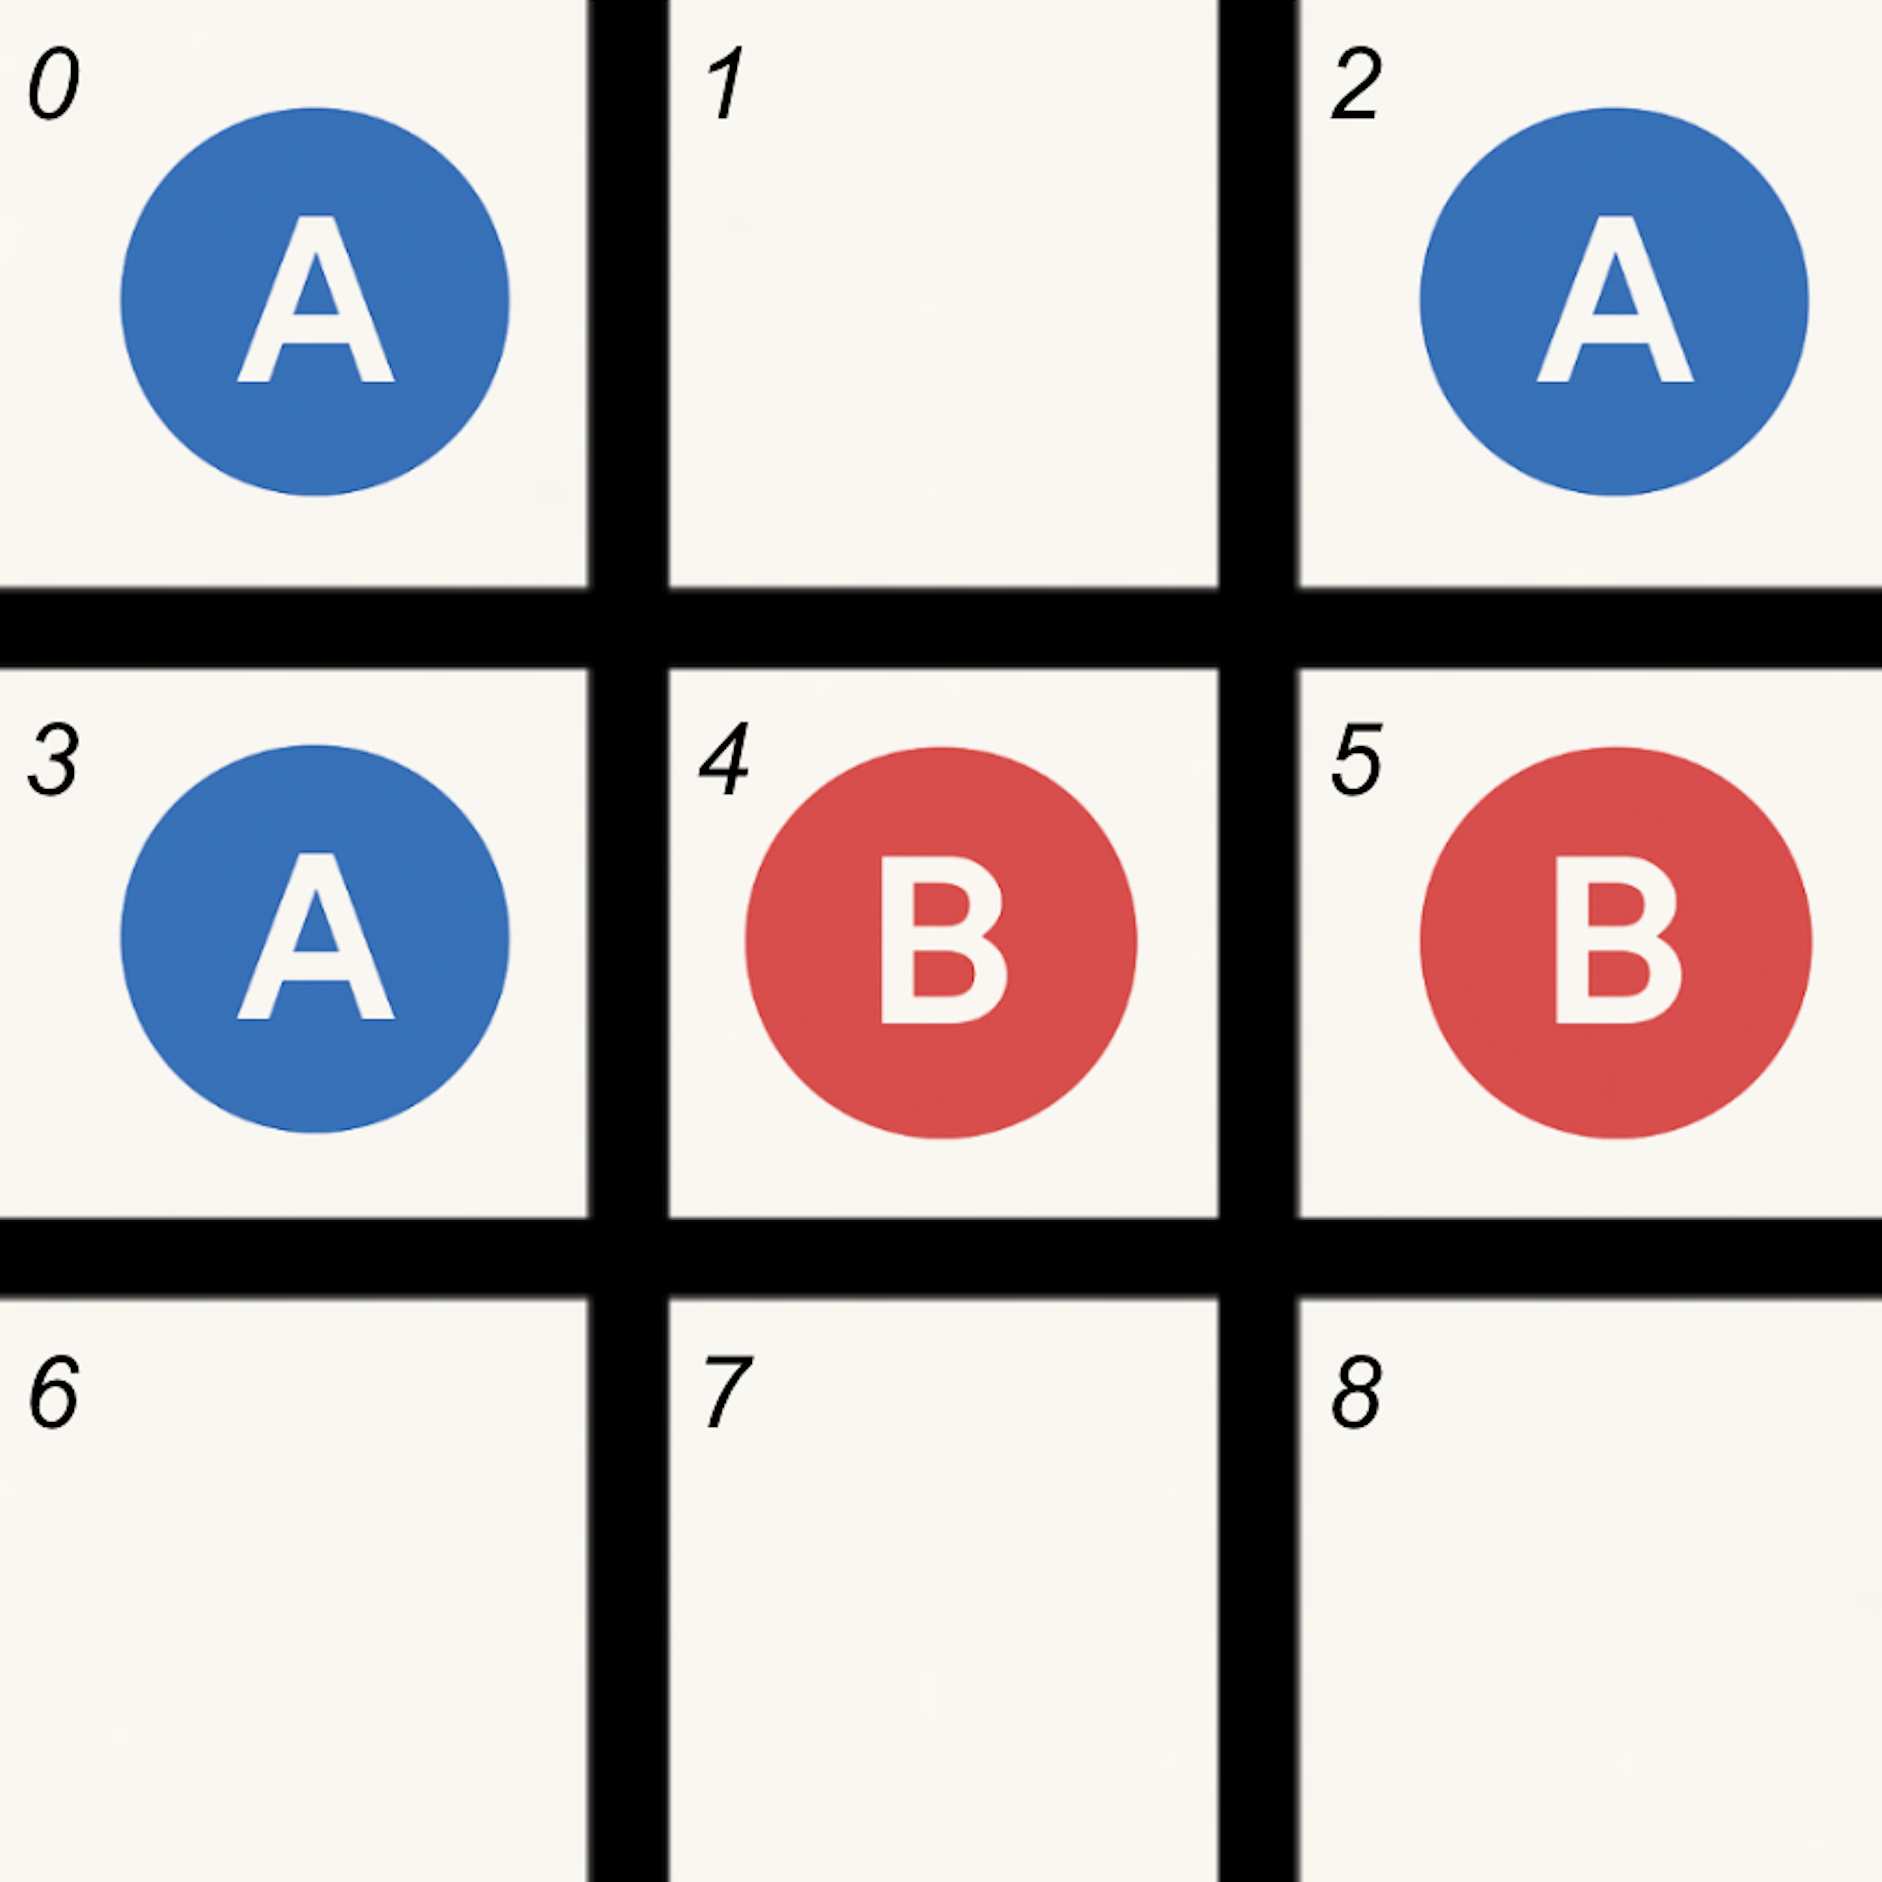
\includegraphics[width=0.5\textwidth,keepaspectratio]{inserted_images/p1_p2_board_edit.png}
\end{center}

But, in a Me/You system, the current player is Player B, so Player B's
tokens are counted as Me and Player A's are counted as You:

\begin{center}
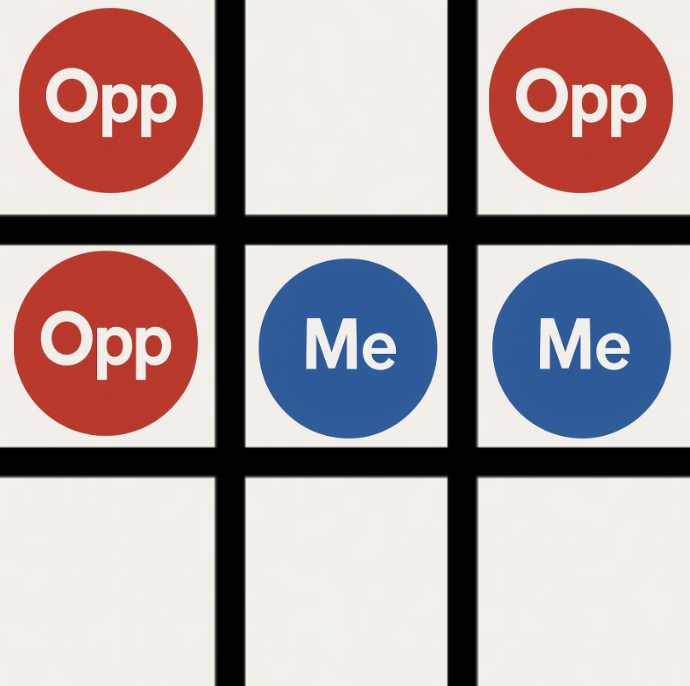
\includegraphics[width=0.5\textwidth,keepaspectratio]{inserted_images/me_opp_board.png}
\end{center}

Now, observe what happens when we add another move to the game, making
our input sequence \texttt{{[}9,\ 2,\ 5,\ 3,\ 4,\ 0,\ 7{]}}. The
original moves on the Player A/Player B board are unchanged:

\begin{center}
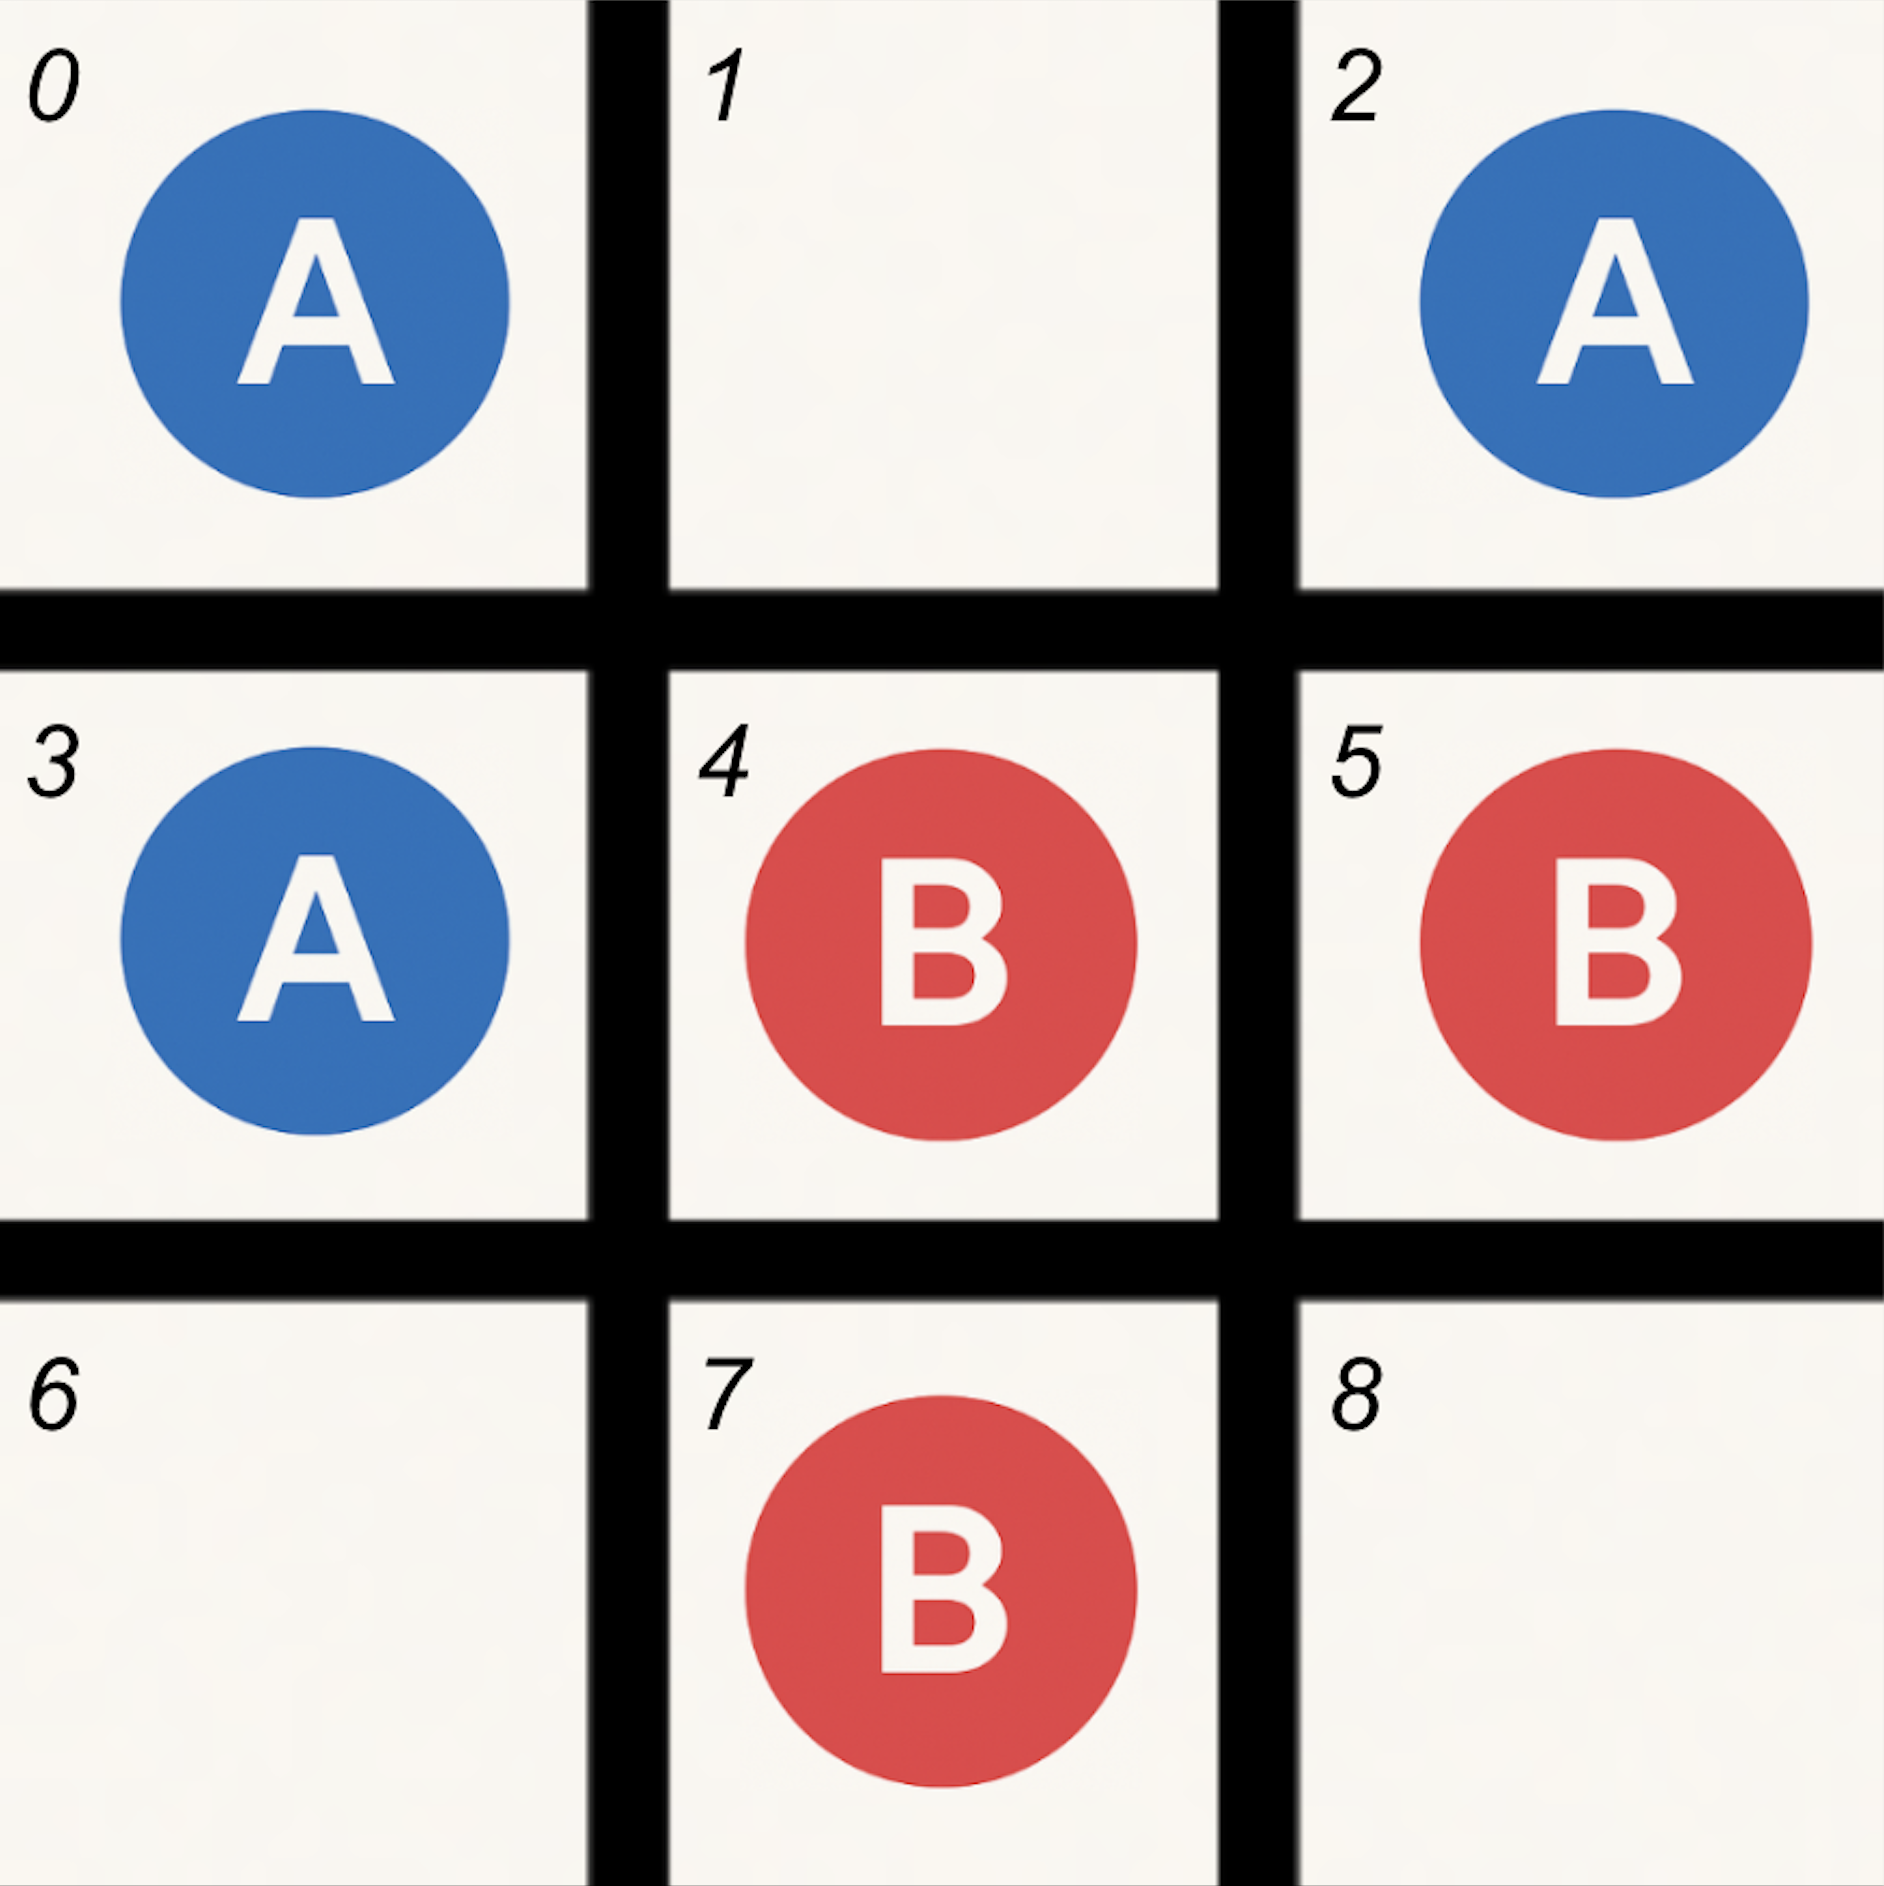
\includegraphics[width=0.5\textwidth,keepaspectratio]{inserted_images/p1_p2_board_update_edit.png}
\end{center}

But, the original moves on the Me/You board have flipped, because the
current player is now Player A:

\begin{center}
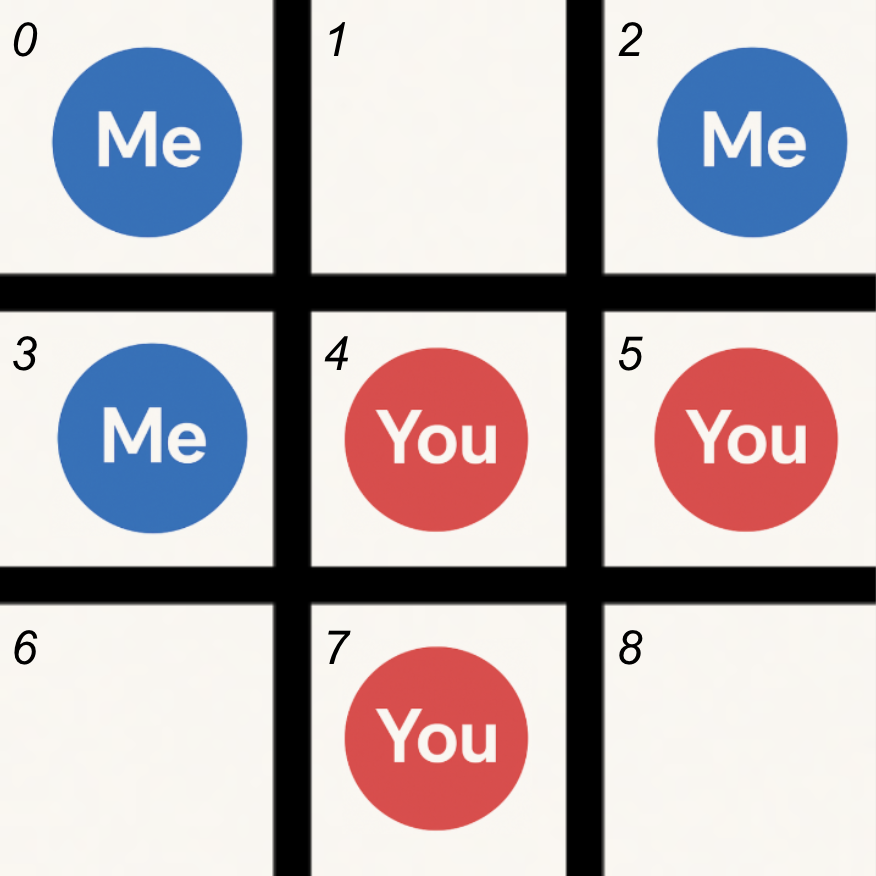
\includegraphics[width=0.5\textwidth,keepaspectratio]{inserted_images/me_opp_board_update.png}
\end{center}

We'll use this modified task later on, so make sure you understand the
difference.

    \subsubsection{Our Questions}\label{our-questions}

Based on these two studies of OthelloGPT, we attempt to apply a version
of probing to our model. Our main goal is to understand more about the
two-stage learning the model exhibits, and to do so, we ask three
questions:

\begin{enumerate}
\def\labelenumi{\arabic{enumi}.}
\tightlist
\item
  Does our model learn an internal representation of the board state,
  like OthelloGPT?
\item
  Is this representation linear or nonlinear?
\item
  How does the internal representation change when the model is at
  different stages of the training process? And specifically, what
  happens before and after the model stalls with a validation loss in
  the 1.36-1.37 range?
\end{enumerate}

\subsubsection{Different Tasks to Test}\label{different-tasks-to-test}

To learn more about our model's behavior, we define four tasks to test
our probe on. The first two directly mirror Rule 1 and Rule 2 of
tic-tac-toe, which we defined earlier. We know that the model learns to
follow Rule 1 by the time stalling begins, and learns to follow Rule 2
by the time stalling ends, so these tasks serve primarily as sanity
checks. They confirm that the model's behavior aligns with the rules of
the game, but don't necessarily indicate that it has formed an internal
representation of the board.

The next two tasks go further. They focus on the identity of the player
occupying each space, and allow us to directly compare the
classification tasks from the original OthelloGPT paper and Nanda's
update. Successful performance here would suggest that the model has
developed an internal representation of the board state, one that
captures who played where. It's important to remember that we never told
the model there were two different players, or even that there was a
board with different spaces. All it saw during training was a sequence of
tokens, with the goal of predicting the next one. If probes succeed at
this task, it suggests that the model might have developed an internal
representation of game state purely through training to do next-token
prediction.

The tasks are defined below:

\begin{enumerate}
\def\labelenumi{\arabic{enumi}.}
\tightlist
\item
  \textbf{Space Occupancy}: What spaces are occupied?
\item
  \textbf{Win Detection}: Has the game been won?
\item
  \textbf{A/B Occupancy}: Which player has played in each space, using
  Player A's vs Player B's space?
\item
  \textbf{Me/You Occupancy}: Which player has played in each space,
  using Me vs You space?
\end{enumerate}

    \subsubsection{Different Probe
Architectures}\label{different-probe-architectures}

We also want to be sure that if there are differences in performance
between linear and nonlinear probes, this difference is due to the
nonlinearity of the internal representation, not just that nonlinear
probes have more parameters and are thus more powerful.\footnote{The size of the linear vs.~nonlinear probes is actually not
mentioned in the original Othello paper, so this is an important new
addition for us to test.} In
order to test this, we use three probes: a linear probe, a small MLP,
and a large MLP. The number of parameters for each model and task are
shown in the table below:

\begin{longtable}[]{@{}
  >{\raggedright\arraybackslash}p{(\linewidth - 8\tabcolsep) * \real{0.3043}}
  >{\raggedright\arraybackslash}p{(\linewidth - 8\tabcolsep) * \real{0.1739}}
  >{\raggedright\arraybackslash}p{(\linewidth - 8\tabcolsep) * \real{0.1739}}
  >{\raggedright\arraybackslash}p{(\linewidth - 8\tabcolsep) * \real{0.1739}}
  >{\raggedright\arraybackslash}p{(\linewidth - 8\tabcolsep) * \real{0.1739}}@{}}
\toprule\noalign{}
\begin{minipage}[b]{\linewidth}\raggedright
\end{minipage} & \begin{minipage}[b]{\linewidth}\raggedright
Space Occupancy
\end{minipage} & \begin{minipage}[b]{\linewidth}\raggedright
Win Detection
\end{minipage} & \begin{minipage}[b]{\linewidth}\raggedright
A/B Occupancy
\end{minipage} & \begin{minipage}[b]{\linewidth}\raggedright
Me/You Occupancy
\end{minipage} \\
\midrule\noalign{}
\endhead
\bottomrule\noalign{}
\endlastfoot
Linear & 351 & 26 & 351 & 351 \\
Small MLP & 507 & 182 & 507 & 507 \\
Large MLP & 1403 & 978 & 1403 & 1403 \\
\end{longtable}

For most tasks, the small MLP is closer in number of parameters to the
linear model than it is to the large MLP. This means that if we see a
large performance gap between the linear model and the small MLP, but a
small performance gap between the small MLP and the large MLP, we can
probably attribute the difference to an inherently nonlinear
representation, not a more complex probe.

    \subsubsection{Results Part 1: Internal Representation Existence and
Linearity}\label{results-part-1-internal-representation-existence-and-linearity}

In order to train the probes on activation-board pairs, we need to train
a GPT to generate these pairs. The training run for the GPT used to
generate probing data is displayed below. Circled locations are where
checkpoints were taken. From left to right, the checkpoints represent
key moments in training:

\begin{itemize}
\tightlist
\item
  A \textbf{Random} model (Checkpoint 1) with weights initialized before
  any training
\item
  The model where \textbf{Stalling Begins} (Checkpoint 2), when
  validation loss first hits 1.37 and stalling behavior begins
\item
  The model where \textbf{Stalling Ends} (Checkpoint 3), as validation
  loss reaches 1.36 and stalling behavior ends
\item
  The \textbf{Fully Trained} model (Checkpoint 4) after 100,000
  iterations
\end{itemize}

\begin{center}
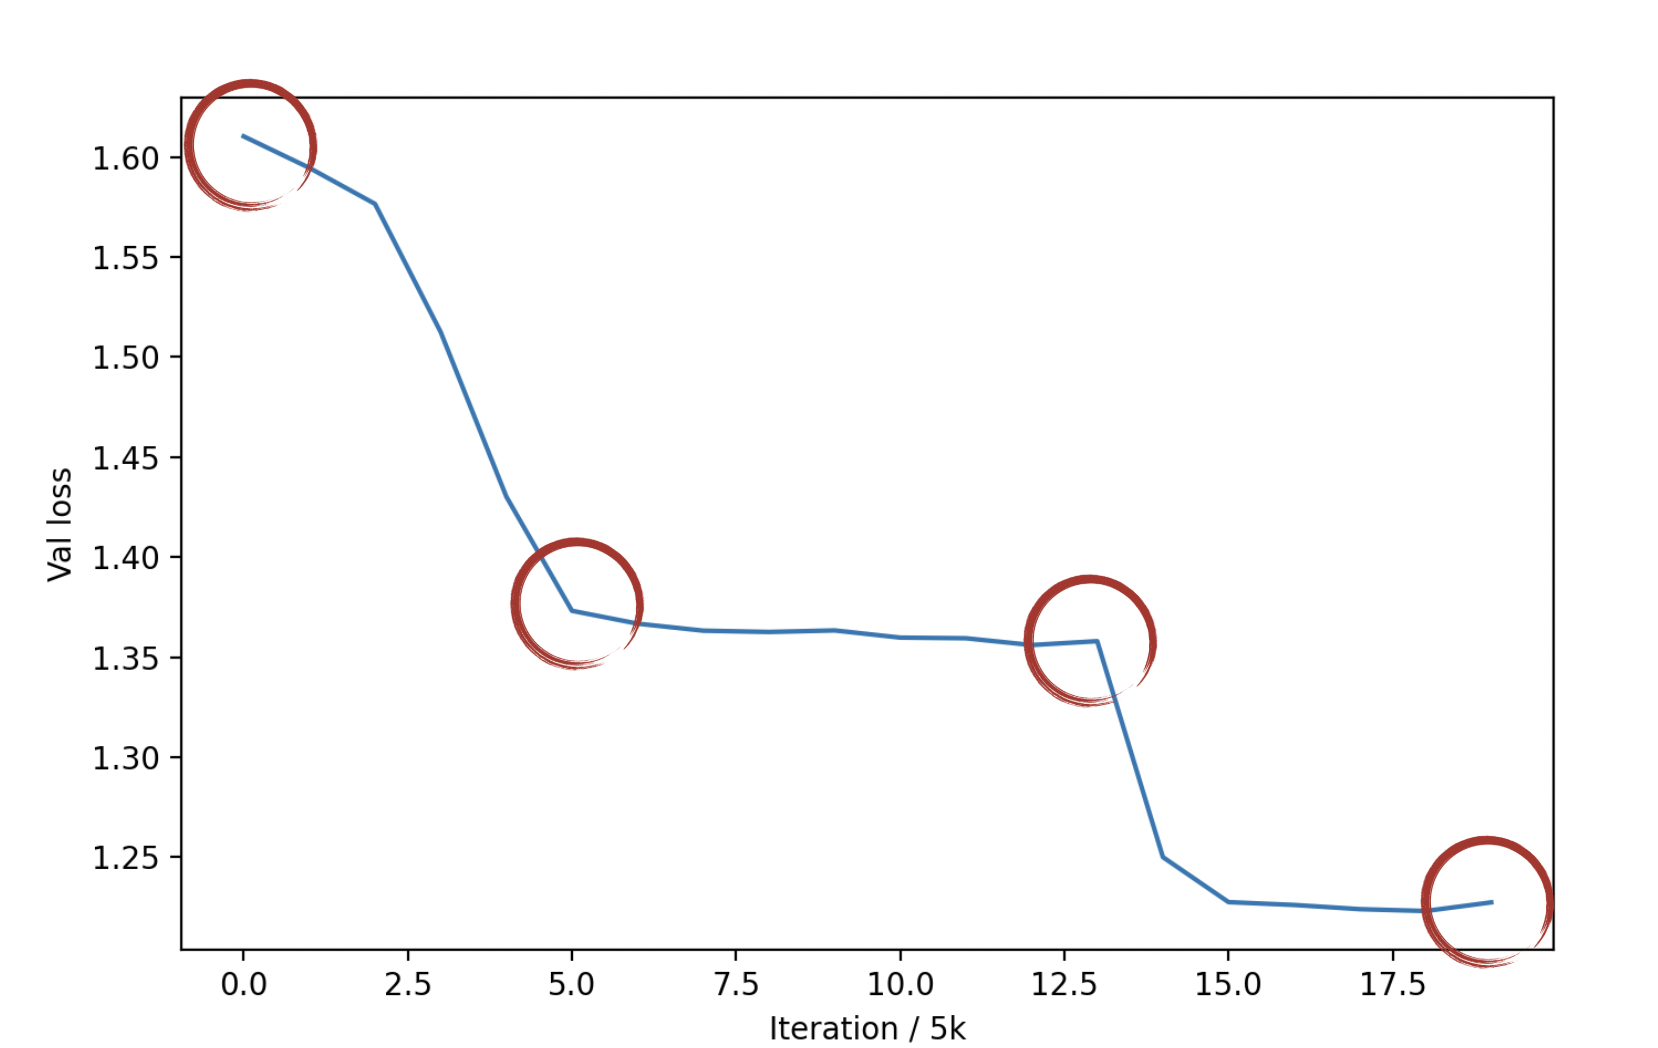
\includegraphics[width=1\textwidth,keepaspectratio]{inserted_images/checkpoint_locs.png}
\end{center} 

    To generate data, we begin by loading the trained GPT model at each of
the four checkpoints. We use a dataset consisting of full tic-tac-toe
games, each encoded as a sequence of tokens as discussed in the Model
Representation section. These sequences represent complete games, but we
do not feed the entire sequence to the model all at once. Instead, for
each game, we create a series of 10 truncated input sequences: the first
contains only the start token, the second contains the start token
followed by the first move, the third includes the first two moves, and
so on, up to the full sequence of 10 tokens. This results in 10 distinct
input sequences per game, each representing a partial progression of the
game state.

Each of these input sequences is fed through the model, and we extract
the corresponding internal activations after three layers of the model:

\begin{enumerate}
\def\labelenumi{\arabic{enumi}.}
\tightlist
\item
  The \textbf{Embedding} layer
\item
  The \textbf{Transformer} block
\item
  The final \textbf{LayerNorm} after the transformer.
\end{enumerate}

These activations become the input features used to train the probing
models.

The corresponding ground truth labels are derived directly from the
input sequences by decoding the tokenized moves to reconstruct the board
state at that point in the game. Depending on the specific probing task,
the label is either a classification for each of the 9 spaces on the
board (e.g., predicting whether a space is X, O, or empty), or a binary
label indicating whether the board has a winner. This procedure is
repeated independently for each checkpoint, enabling us to compare how
the internal representations evolve over the course of training.

Once the probing data is generated, we are left with a distinct dataset
for each combination of checkpoint and layer: one for the embedding
layer, one for the first transformer block, and one for the final
LayerNorm layer, at each of the four checkpoints. Each of these datasets
is split into a training set of 100,000 examples and a validation set of
20,000 examples. We train a separate probe on the training portion of
each dataset and evaluate it on the corresponding validation set. For
Space Occupancy, A/B Occupancy, and Me/You occupancy, we compute space
accuracy, defined as the percentage of individual board spaces the probe
correctly classifies. For Win Detection, we compute board-level
accuracy, which measures how often the probe correctly determines
whether or not the board contains a winner.

Results of this experiment are shown in tables below. In this section,
we'll focus on whether there is an internal representation, whether it
is linear, and where within the model this representation is learned.
The results compare four probes: a linear, a small MLP, and a large MLP
using data from the \textbf{Fully Trained} Checkpoint and a large MLP
using data from the \textbf{Random} Checkpoint. Because this is a
randomly initialized model, this large MLP probe serves as a baseline of
how well the most powerful probe can do using activations from an
untrained model. We can compare the other three probes trained on
\textbf{Fully Trained} data to this baseline to understand how much the
GPT's internal representation improves during training.

    \paragraph{Task 1: Space Occupancy}\label{task-1-space-occupancy}

\begin{longtable}[]{@{}llll@{}}
\toprule\noalign{}
Probe Type & Embedding & Transformer & LayerNorm \\
\midrule\noalign{}
\endhead
\bottomrule\noalign{}
\endlastfoot
Linear & 0.774 & 0.936 & 0.943 \\
Small MLP & 0.788 & 0.953 & 0.973 \\
Large MLP & 0.788 & 0.977 & 0.988 \\
Large MLP (Baseline) & 0.760 & 0.764 & 0.829 \\
\end{longtable}

\textbf{1. Does the GPT learn Rule 1?}\\
\emph{Yes}. By the LayerNorm, all three probes trained on the Fully
Trained checkpoint greatly outperform the baseline probe. As expected,
probes trained on this model are able to identify which spaces are
occupied. Since the model learns not to play in occupied spaces, and we
can extract that information from its activations, this suggests it
encodes this rule as it learns.

\textbf{2. Where is this rule learned?}\\
It seems to be mostly learned the transformer layer. This is where we
see probe accuracy spike.

\textbf{3. Is this representation linear?}\\
\emph{Mostly}. The linear probe is able to make predictions that are
nearly as accurate as either of the MLP probes. The nonlinear probes do
slightly outperform the linear probe, so the GPT's representation of
this rule may contain some mild nonlinearity.

    \paragraph{Task 2: Win Detection}\label{task-2-win-detection}

\begin{longtable}[]{@{}llll@{}}
\toprule\noalign{}
Probe Type & Embedding & Transformer & LayerNorm \\
\midrule\noalign{}
\endhead
\bottomrule\noalign{}
\endlastfoot
Linear & 0.924 & 0.919 & 0.954 \\
Small MLP & 0.925 & 0.986 & 0.986 \\
Large MLP & 0.922 & 0.987 & 0.988 \\
Large MLP (Baseline) & 0.912 & 0.922 & 0.924 \\
\end{longtable}

\textbf{1. Does the GPT learn Rule 2?}\\
\emph{Yes}. By the LayerNorm, all three probes trained on the Fully
Trained Checkpoint greatly outperform the baseline probe. As expected,
probes trained on this model are able to identify whether a game has a
winner. Since the model learns to detect winners, and we can extract
that information from its activations, this suggests it encodes this
rule as it learns.

\textbf{2. Where is this rule learned?}\\
The MLP probes learn this rule by the transformer layer. However, the
linear probe only achieves accuracy above baseline at the LayerNorm.

\textbf{3. Is this representation linear?}\\
\emph{Somewhat}. The MLP probes perform similarly to each other, and far
outperform the linear probe, but the linear probe does substantially
outperform the baseline probe. The fact that the MLP probes learn the
internal represenation before Layer 3, while the linear probe does not,
suggests that the GPT's LayerNorm removes some, but not all, of the
nonlinearity of the representation. This could explain why the linear
probe performs better after the LayerNorm than after the transformer
block.

    \paragraph{Task 3: A/B Occupancy}\label{task-3-ab-occupancy}

\begin{longtable}[]{@{}llll@{}}
\toprule\noalign{}
Probe Type & Embedding & Transformer & LayerNorm \\
\midrule\noalign{}
\endhead
\bottomrule\noalign{}
\endlastfoot
Linear & 0.609 & 0.729 & 0.732 \\
Small MLP & 0.620 & 0.783 & 0.778 \\
Large MLP & 0.665 & 0.796 & 0.798 \\
Large MLP (Baseline) & 0.663 & 0.674 & 0.698 \\
\end{longtable}

\textbf{1. Is there an internal representation?}\\
\emph{Yes}. By the LayerNorm, both MLP probes trained on the Fully
Trained Checkpoint greatly outperform the baseline probe, and the linear
probe slightly outperforms baseline. This suggests the GPT learns some
internal representation of space occupancy from a Player A-Player B
perspective.

\textbf{2. Where is this representation learned?}\\
All three probes learn this representation by the transformer layer. The
LayerNorm does not further increase probe accuracy.

\textbf{3. Is this representation linear?}\\
\emph{No}. The MLP probes perform similarly to each other, and far
outperform the linear probe. The linear probe does perform better than
baseline, but not substantially so.

    \paragraph{Task 4: Me/You Occupancy}\label{task-4-meyou-occupancy}

\begin{longtable}[]{@{}llll@{}}
\toprule\noalign{}
Probe Type & Embedding & Transformer & LayerNorm \\
\midrule\noalign{}
\endhead
\bottomrule\noalign{}
\endlastfoot
Linear & 0.642 & 0.768 & 0.833 \\
Small MLP & 0.668 & 0.877 & 0.871 \\
Large MLP & 0.670 & 0.900 & 0.901 \\
Large MLP (Baseline) & 0.667 & 0.637 & 0.697 \\
\end{longtable}

\textbf{1. Is there an internal representation?}\\
\emph{Yes}. By the LayerNorm, all three probes trained on the Fully
Trained Checkpoint greatly outperform the baseline probe. This suggests
the GPT learns an internal representation of space occupancy from a
me-you perspective.

\textbf{2. Where is this representation learned?}\\
The MLP probes learn this representation by the transformer layer. The
linear probe achieves accuracy over baseline by the transformer layer,
but is substantially more accurate after the LayerNorm.

\textbf{3. Is this representation linear?}\\
\emph{Somewhat}. The MLP probes perform similarly to each other, and far
outperform the linear probe. The linear model does, however, perform
substantially better than baseline. The increase in the linear probe's
performance between Layer 2 and Layer 3 suggests that the GPT's
LayerNorm removes some nonlinearity from its internal representation,
making it more accessible to linear probes.

    \paragraph{Overall summary}\label{overall-summary}

The success of the probes suggests the GPT model develops internal
representations, even though it was not explicitly trained to do so.
These representations are largely formed in the transformer layer, with
the LayerNorm layer sometimes refining them and making them more
accessible to linear probes. For all occupancy tasks, we see a
noticeable spike in accuracy for all probe types at the transformer
layer, indicating that it encodes relevant information. For Win
Detection and A/B occupancy, the LayerNorm layer further boosts linear
probe performance, suggesting that it helps transform these nonlinear
representations that the transformer produces into a more linearly
decodable form. While linear probes consistently outperform the
baseline, they are typically outperformed by both the small and large
MLP probes. This pattern, observed across all tasks, suggests that the
internal representations are only partially linear.

For the two rule-based tasks (Space Occupancy and Win Detection), strong
probe performance was expected, as the GPT eventually learned to play by
these two rules. We observed this expected strong probe performance,
aligning with the low invalid move rate and high correct ending rate we
observed in the previous section and confirming that the model has
learned to behave according to the rules of tic-tac-toe.

In the two player-identity tasks (A/B Occupancy and Me/You Occupancy),
probe performance provides strong evidence of an internal representation
of board state. These tasks require our probes to use model activations
to infer not just what moves have been made, but who made them. This
information that was never explicitly provided during training, nor was
it a given task for the GPT to learn a representation. However,
performance well above baseline probes suggests that during training,
the GPT develops an internal representation of the game to help with
next-token prediction.

A/B occupancy and Me/You occupancy also mirror the tasks tested by the
OthelloGPT team and Nanda, respectively. Consistent with Nanda's work,
all probe types perform better on the Me/You task than on the A/B task.
This supports the idea that the model interprets and represents the
board from the perspective of the \emph{current player}. However, our
results diverge from Nanda's in a key way: while Nanda concluded that
A/B occupancy could be fully represented with a linear probe, we find
that the nonlinear probes still substantially outperform the linear
probe in this setting. This indicates that the GPT's internal
representation of the Me/You task is still meaningfully nonlinear. This
result aligns more closely with conclusions from the OthelloGPT team,
who found that nonlinear probes are needed to access the model's
internal board state representations.

    \subsubsection{Results Part 2: Changes in Internal Representation During
Training}\label{results-part-2-changes-in-internal-representation-during-training}

Now that we know that the GPT eventually learns an internal
representation of the game state, we'll explore how this representation
develops as the model trains. Recall the two rules we defined for
tic-tac-toe. In particular, we observed that the GPT first learns to not
play in occupied spaces (Rule 1) at the Stalling Begins checkpoint, and
later learns to correctly identify the end of games (Rule 2) at the
Stalling Ends checkpoint. These changes in behavior are expected, but do
they correspond to actual shifts in the model's internal
representations? How do the internal representations change during
training?

We test this by comparing the performance of each probe type (Linear,
Small MLP, Large MLP) on our four tasks across checkpoints. Space
Occupancy explicitly tests model understanding of Rule 1, and Win
Detection explicitly tests model understanding of Rule 2. A/B Occupancy
and Me/You Occupancy involve understanding and representing the entire
board state, so they provide a more complete test of whether and how the
model internalizes the structure of the game.

Presented below are tables for the accuracies of probes trained on each
checkpoint from activations taken from the LayerNorm of the GPT, as well
as a chart showing how each probe's performance changes across
checkpoints. We'll discuss the results below.

    \paragraph{Linear Probe}\label{linear-probe}

\begin{longtable}[]{@{}
  >{\raggedright\arraybackslash}p{(\linewidth - 8\tabcolsep) * \real{0.1515}}
  >{\raggedright\arraybackslash}p{(\linewidth - 8\tabcolsep) * \real{0.2121}}
  >{\raggedright\arraybackslash}p{(\linewidth - 8\tabcolsep) * \real{0.2121}}
  >{\raggedright\arraybackslash}p{(\linewidth - 8\tabcolsep) * \real{0.2121}}
  >{\raggedright\arraybackslash}p{(\linewidth - 8\tabcolsep) * \real{0.2121}}@{}}
\toprule\noalign{}
\begin{minipage}[b]{\linewidth}\raggedright
Task
\end{minipage} & \begin{minipage}[b]{\linewidth}\raggedright
Random
\end{minipage} & \begin{minipage}[b]{\linewidth}\raggedright
Stalling Begins
\end{minipage} & \begin{minipage}[b]{\linewidth}\raggedright
Stalling Ends
\end{minipage} & \begin{minipage}[b]{\linewidth}\raggedright
Fully Trained
\end{minipage} \\
\midrule\noalign{}
\endhead
\bottomrule\noalign{}
\endlastfoot
Space Occupancy & 0.660 & 0.948 & 0.932 & 0.943 \\
Win Detection & 0.900 & 0.920 & 0.954 & 0.954 \\
A/B Occupancy & 0.569 & 0.745 & 0.734 & 0.732 \\
Me/You Occupancy & 0.587 & 0.750 & 0.824 & 0.833 \\
\end{longtable}

\paragraph{Small MLP Probe}\label{small-mlp-probe}

\begin{longtable}[]{@{}
  >{\raggedright\arraybackslash}p{(\linewidth - 8\tabcolsep) * \real{0.1515}}
  >{\raggedright\arraybackslash}p{(\linewidth - 8\tabcolsep) * \real{0.2121}}
  >{\raggedright\arraybackslash}p{(\linewidth - 8\tabcolsep) * \real{0.2121}}
  >{\raggedright\arraybackslash}p{(\linewidth - 8\tabcolsep) * \real{0.2121}}
  >{\raggedright\arraybackslash}p{(\linewidth - 8\tabcolsep) * \real{0.2121}}@{}}
\toprule\noalign{}
\begin{minipage}[b]{\linewidth}\raggedright
Task
\end{minipage} & \begin{minipage}[b]{\linewidth}\raggedright
Random
\end{minipage} & \begin{minipage}[b]{\linewidth}\raggedright
Stalling Begins
\end{minipage} & \begin{minipage}[b]{\linewidth}\raggedright
Stalling Ends
\end{minipage} & \begin{minipage}[b]{\linewidth}\raggedright
Fully Trained
\end{minipage} \\
\midrule\noalign{}
\endhead
\bottomrule\noalign{}
\endlastfoot
Space Occupancy & 0.790 & 0.979 & 0.960 & 0.973 \\
Win Detection & 0.923 & 0.921 & 0.987 & 0.986 \\
A/B Occupancy & 0.649 & 0.769 & 0.755 & 0.778 \\
Me/You Occupancy & 0.661 & 0.772 & 0.855 & 0.871 \\
\end{longtable}

\paragraph{Large MLP Probe}\label{large-mlp-probe}

\begin{longtable}[]{@{}
  >{\raggedright\arraybackslash}p{(\linewidth - 8\tabcolsep) * \real{0.1515}}
  >{\raggedright\arraybackslash}p{(\linewidth - 8\tabcolsep) * \real{0.2121}}
  >{\raggedright\arraybackslash}p{(\linewidth - 8\tabcolsep) * \real{0.2121}}
  >{\raggedright\arraybackslash}p{(\linewidth - 8\tabcolsep) * \real{0.2121}}
  >{\raggedright\arraybackslash}p{(\linewidth - 8\tabcolsep) * \real{0.2121}}@{}}
\toprule\noalign{}
\begin{minipage}[b]{\linewidth}\raggedright
Task
\end{minipage} & \begin{minipage}[b]{\linewidth}\raggedright
Random
\end{minipage} & \begin{minipage}[b]{\linewidth}\raggedright
Stalling Begins
\end{minipage} & \begin{minipage}[b]{\linewidth}\raggedright
Stalling Ends
\end{minipage} & \begin{minipage}[b]{\linewidth}\raggedright
Fully Trained
\end{minipage} \\
\midrule\noalign{}
\endhead
\bottomrule\noalign{}
\endlastfoot
Space Occupancy & 0.829 & 0.991 & 0.970 & 0.988 \\
Win Detection & 0.924 & 0.922 & 0.988 & 0.988 \\
A/B Occupancy & 0.698 & 0.779 & 0.778 & 0.798 \\
Me/You Occupancy & 0.697 & 0.792 & 0.879 & 0.901 \\
\end{longtable}

\paragraph{Results Plotted}\label{results-plotted}

\vspace{1em}

\begin{center}
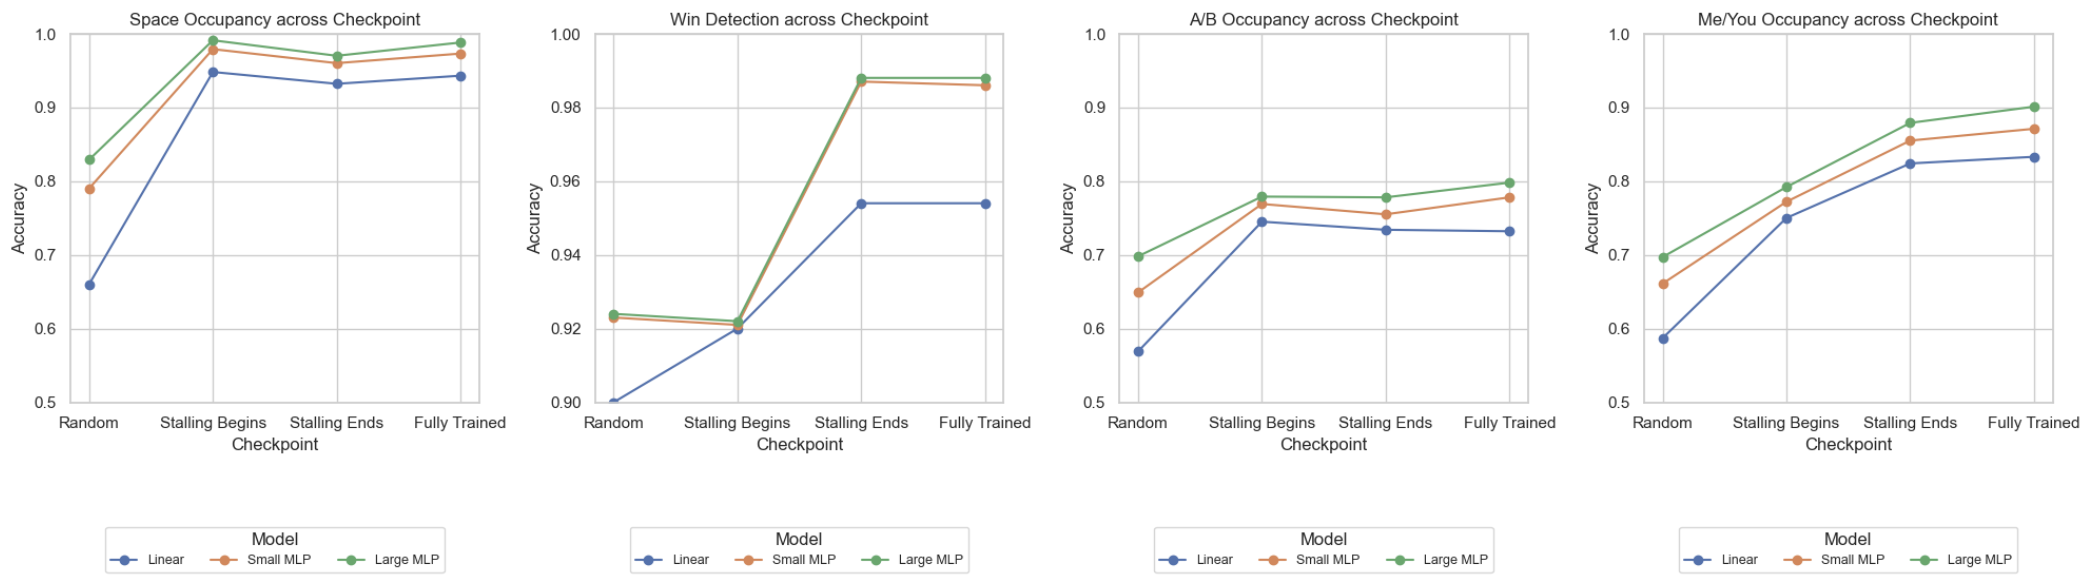
\includegraphics[width=\textwidth, keepaspectratio]{inserted_images/labeled_accuracy_by_checkpoint_key.png}
\end{center}
    \paragraph{Observations}\label{observations}

Take a look at the tables and chart above, and focus on the transition
between Stalling Begins and Stalling Ends. As we discussed, this is
where the GPT's behavior shifts. At the Stalling Begins checkpoint, the
model has learned not to play invalid moves but cannot identify when the
game has ended (invalid move rate is low, but correct ending rate is
also low), but at the Stalling Ends checkpoint, it learns to identify
when games have ended (the correct ending rate is now high) . This
progression aligns with our two defined rules of tic-tac-toe. Space
Occupancy (Rule 1) and Win Detection (Rule 2) help isolate the internal
representation of each rule, while A/B Occupancy and Me/You Occupancy
depend on a composition of both.

By the Stalling Begins checkpoint, Space Occupancy performance is
already nearly perfect for all probe types, especially for the nonlinear
probes. This is expected, since the GPT plays according to Rule 1 by
this point, but the probe performance confirms that the rule is also
internally represented. In contrast, performance on Win Detection does
not improve until the Stalling Ends checkpoint, where it jumps to nearly
perfect performance, especially for the MLP probes. This shift in Win
Detection accuracy mirrors the point at which the GPT starts identifying
game ends correctly, suggesting that the internal representation of Rule
2 is not present until this later checkpoint.

A/B and Me/You Occupancy both require an understanding of both Rule 1
and Rule 2, but they show different patterns. Probes trained on A/B
Occupancy see a jump from the Random checkpoint to the Stalling Begins
checkpoint, then plateau, while Me/You Occupancy probes show steady
improvement throughout training. We see jumps in Me/You Occupancy
performance as each rule is learned, suggesting that as the model learns
how to play, it also learns to internally represent the board. Notably,
all probe types perform better on Me/You Occupancy than A/B Occupancy,
supporting the idea that the GPT internally understands the game through
this lens.

Taken together, these results highlight that the GPT's internal
representation of game state evolves in distinct phases. First, it
learns to represent Space Occupancy (Rule 1) by the Stalling Begins
checkpoint, then it learns to represent Win Detection (Rule 2) by the
Stalling Ends checkpoint. As these rule representations improve, so does
probe accuracy on Me/You Occupancy. This suggests that learning the
rules improves not just the model's behavior, but also its internal
representation of the game state. Importantly, the probes help us
understand not just \emph{that} the model behaves differently, but
\emph{why} it performs differently, by revealing when different
understandings of the board state become represented internally by the
model. The probing tasks allow us to track these representational
changes during training, and the difference in Me/You occupancy probe
performance before and after stalling behavior offers strong evidence
that the changes in model behavior we observed reflect changes in the
model's internal encoding of the game. While the model could in theory
behave correctly without any internal representation of the game, the
probes show that such a representation does, in fact, emerge and evolve
over training.

    \section{Conclusion}\label{conclusion}

\subsection{Summary of Findings}\label{summary-of-findings}

In this project, we trained a GPT to generate valid moves and complete
games of tic-tac-toe. We were interested in three main questions:

\begin{enumerate}
\def\labelenumi{\arabic{enumi}.}
\tightlist
\item
  Does the model generate novel games, or just memorize games that it
  was shown?
\item
  How does this learning occur?
\item
  Is there an internal representation of the game? Does it change as the
  model learns?
\end{enumerate}

To answer the first question, we looked at the full games the model
generated and observed what proportion of those were included in the
training dataset, and what proportion were original. We found that the
model generated original games at around the frequency we'd expect of a
model without any memorization, so we concluded that the model was not
memorizing, but instead was learning to play tic-tac-toe legally.

To address the second question, we tracked how the model learned over
time. In more than 70\% of successful training runs, the model's loss
decreases in two distinct stages. Each of these stages corresponds to
one of the two rules of tic-tac-toe:

\begin{enumerate}
\def\labelenumi{\arabic{enumi}.}
\tightlist
\item
  Play a piece in an unoccupied space.
\item
  If one player places three of their pieces in a row, they win.
\end{enumerate}

After the first stage, the model learns to avoid illegal moves where it
attempts to play in an already-occupied space (Rule 1). After the second
stage, the model learns to recognize when a player has won by
occupying three spaces in a row and stops predicting additional moves,
instead predicting the padding token used to signify the end of a game
(Rule 2). These shifts in behavior suggest that the model somehow
internalizes the basic rules of tic-tac-toe, first learning how to play
legally, then learning how the game ends.

For our final question, we were interested in understanding more about
how the model learns the rules of the game. To do so, we trained linear
and nonlinear probes on the GPT's activations to see if the GPT
developed an internal representation of the board state, and if this
representation changed throughout training. We defined four probing
tasks: Space Occupancy and Win Detection reflected the rules of
tic-tac-toe we defined earlier. A/B Occupancy and Me/You Occupancy
involved identifying which player occupied each square (with different
framing) and tested understanding of the entire board. While the first
two tasks helped confirm that the model was behaving according to the
rules, the second two were more reflective of whether the model had
developed a full internal representation of game state. For each of
these tasks, probes trained on activations from a fully trained GPT
outperformed probes trained on activations from an untrained GPT,
suggesting that the GPT learned an internal representation of the board.
Importantly, the model was not tasked with learning this internal
representation, only generating the next valid move, but the
representation developed anyway. We tracked the success of the probes
across layers and found that this representation was primarily learned
by the transformer layer. Because nonlinear probes consistently
outperformed linear probes, it seems that this representation is
somewhat nonlinear. Improvement in linear probes after the final
LayerNorm suggests that this layer removes some nonlinearity from the
model's internal representations. Finally, we observed that the internal
representation evolved as the GPT trained, and the game state
information our probes were able to extract matched the model's
generation capabilities at the training stage from which the probe was
trained.

Tic-tac-toe isn't exactly language generation, but we studied our GPT
using techniques that are often used in mechanistic interpretability
research on LLMs like ChatGPT. We tested for model originality and
memorization, tracked different metrics for learning as the model
trained, and introduced probes to investigate how the model internalized
its understanding of the game. Of course, GPTs trained on natural
language are vastly more complex models trying to learn a much more
ambiguous task. They don't have explicit rules like tic-tac-toe, and
their internal representations are shaped by more varied objectives and
data. Still, we can apply a similar sort of study: by training a model
on next-token prediction, we can begin to uncover how the architecture
supports generalization, rule learning, and internal representation.
This project shows that even tiny GPTs, trained on simple data, can
develop accurate internal representations. These toy models offer an
environment where we can test hypotheses, develop tools, and build
intuition that may eventually scale to more complex work.

    \subsection{Future Work}\label{future-work}

While I'm satisfied with my findings in this project, there were a
number of tasks/questions I wanted to look into, but didn't have the
time to accomplish. I've detailed some avenues for future work below:

\subsubsection{\texorpdfstring{Generalization to \emph{mnk}
Games}{Generalization to mnk Games}}\label{generalization-to-mnk-games}

Tic-tac-toe is a special case of an \emph{mnk} game (with \( m = n = k = 3 \)), where players alternate turns on an \( m \times n \) board and aim to control \( k \) consecutive spaces. A natural extension of this project is to explore how the GPT learns to play these \href{https://www.sciencedirect.com/science/article/pii/S0304397520301146}{more complicated} games. I was planning to go in this direction for a while before I noticed the multi-stage learning and decided to investigate that, so my codebase is set up to work with all \emph{mnk} games. Because of that work, it shouldn't be too difficult to extend this project to more general \emph{mnk} cases.


\subsubsection{Minimum Embedding
Dimensionality}\label{minimum-embedding-dimensionality}

As I tested different GPT architecture, I found that a minimum of
12-dimensional embeddings were necessary for the GPT to learn to play
legal games. This mirrors what Haeusler found in his original creation
of TicTacTransformer. However, neither Haeusler nor I propose \emph{why}
12 dimensions might be necessary. This result is especially surprising
because, in theory, 11 dimensions should be sufficient to uniquely
represent each token given that our vocabulary is only 11 words (all
nine moves on the board, the start token, and the pad token). Further
investigation to discover why 12-dimensional embeddings are necessary
could help us further understand the model's learning process.

\subsubsection{Interventions on Internal
Representations}\label{interventions-on-internal-representations}

In addition to training probes on their model's activations, OthelloGPT
team demonstrated that it is possible to causally intervene on a model's
internal representations to manipulate its behavior in predictable ways.
In their experiments, they passed in a game sequence to OthelloGPT, then
edited the model's activations so that their probes would predict a
different board state from the one that was inputted. Using these new
activations, the model was told to predict the next move. They found
that the model predicted moves that were legal on the new board state
inferred from the probe, not the original board state given to the
model. This showed that the model's internal representation of game
state was not a byproduct of training, but instead was influential in
shaping its output.

A clear next step for this project is to perform similar interventions
on our GPT. By editing the model's activations so that our probes
predicted a different board state, we could test whether the model's
predictions change in response. For example, if we change the
activations such that a previously occupied space appears empty, and the
model then chooses to place a move there, it would suggest that the
model relies on its internal board representation to decide where to
play. This kind of intervention would help us figure out whether the
internal representations we saw with probes are actually used by the
model to guide its predictions, or if they're just a side effect of
training that happen to be decodable by our probes.

    \section{Acknowledgements}\label{acknowledgements}

First, I want to thank Dr.~Yair Shenfeld, my Honors Thesis advisor. He
has been incredibly helpful throughout this year, giving me advice,
thinking through my experiments with me, and providing important
feedback along the way. I wouldn't have been able to research nearly as
much, or nearly as well, without him. I also want to thank
Dr.~Ritambhara Singh, my second reader, for her help and teaching. Her
CSCI 2952G class was my first introduction to interpretability
techniques in deep learning, and the content that I learned helped
inspire parts of this project.

More generally, this thesis is somewhat of a culmination of my time and
academic work at Brown. I want to thank my friends here for all of the
time they spent with me throughout this entire process (and over our
four years here), and my family for all of their support and
encouragement along the way.

    \section{Appendix}\label{appendix}

Presented here is the math of how a GPT works, as well as a couple of
experiments I ran that didn't fit in exactly with the project I wanted
to present.

\subsection{GPT Math}\label{gpt-math}

\subsubsection{Model Initialization and
Configuration}\label{model-initialization-and-configuration}

The model is instantiated with a configuration that specifies the
following parameters:

\begin{itemize}
\tightlist
\item
  \textbf{\texttt{block\_size\ (BLOCK\_SIZE)}}: the maximum number of
  tokens the model can process.\\
\item
  \textbf{\texttt{vocab\_size\ (VOCAB\_SIZE)}}: the size of the
  vocabulary, representing all possible moves plus special tokens.\\
\item
  \textbf{\texttt{n\_layer\ (LAYER\_COUNT)}}: the number of Transformer
  layers in the model.\\
\item
  \textbf{\texttt{n\_head\ (HEAD\_COUNT)}}: the number of attention
  heads in each Transformer layer.\\
\item
  \textbf{\texttt{n\_embd\ (N\_EMBD)}}: the dimensionality of the token
  and position embeddings.\\
\item
  \textbf{\texttt{mlp\_mult\ (MLP\_MULT)}}: a scalar multiplier
  controlling the hidden size of the MLP layers.
\end{itemize}

The model is instantiated with a configuration that specifies the
following parameters:

We adopt the following indexing convention:\\
- Capitalized names (\texttt{N\_EMBD}, \texttt{VOCAB\_SIZE}, etc.)
denote tensor dimensions.\\
- Lowercase letters of the same name (\texttt{n}, \texttt{v}, etc.) are
used for indexing over those dimensions in pseudocode and equations.
- We use 1-indexing in the mathematical notation

All weight matrices are initialized randomly from a normal distribution
\[
\mathcal{N}\left(0, \frac{0.02}{\sqrt{2 \cdot \texttt{n\_layer}}} \right)
\]

    \subsubsection{Token Embeddings}\label{token-embeddings}

To access token embeddings, the model uses a weight matrix \texttt{W\_e}
with dimensions \texttt{(VOCAB\_SIZE,\ N\_EMBD)}, where each row
\texttt{W\_e{[}i{]}} contains the embedding for the \emph{i}-th item in
the vocabulary.

Given an input sequence \texttt{x} of token indices with shape
\texttt{(TOKEN\_COUNT)}\footnote{\texttt{TOKEN\_COUNT} refers to the number of tokens in the input sequence $x$, not the total vocabulary size. We always have $\texttt{TOKEN\_COUNT} \leq \texttt{block\_size}$ because \texttt{block\_size} is the maximum input size the model will take.}, each token is mapped to its
corresponding embedding from \texttt{W\_e}. This produces a token
embedding matrix \texttt{tok\_emb} with dimensions
\texttt{(T,\ N\_EMBD)}, where each element \texttt{tok\_emb{[}t,\ n{]}}
is obtained by mapping token \texttt{t} to its embedding vector
\texttt{W\_e{[}t{]}}, which has size \texttt{N\_EMBD}.

\begin{Shaded}
\begin{Highlighting}[]
\CommentTok{\# Algorithm: Token Embedding Calculation}
\ControlFlowTok{for}\NormalTok{ each position t }\KeywordTok{in}\NormalTok{ sequence length TOKEN\_COUNT:}
\NormalTok{    tok\_emb\_t ← W\_e[x\_t]  }\CommentTok{\# Retrieve embedding for token x\_t}
\end{Highlighting}
\end{Shaded}

    \subsubsection{Position Embeddings}\label{position-embeddings}

In addition to token embeddings, positional information is added to
indicate each token's position within the sequence. This is achieved
through a position embedding matrix \texttt{W\_p} with dimensions
\texttt{(BLOCK\_SIZE,\ N\_EMBD)}, where each row \texttt{W\_p{[}i{]}}
represents the embedding for position \emph{i}.

For a given sequence of length \texttt{TOKEN\_COUNT}, we retrieve one
position embedding for each token position. This produces a position
embedding matrix \texttt{pos\_emb} of shape
\texttt{(TOKEN\_COUNT,\ N\_EMB)}.

\begin{Shaded}
\begin{Highlighting}[]
\CommentTok{\# Algorithm: Position Embedding Calculation}
\ControlFlowTok{for}\NormalTok{ each position t }\KeywordTok{in}\NormalTok{ sequence length TOKEN\_COUNT:}
\NormalTok{    pos\_emb\_t ← W\_p[t]  }\CommentTok{\# Retrieve position embedding for position t}
\end{Highlighting}
\end{Shaded}

    \subsubsection{Combined Embeddings}\label{combined-embeddings}

The full embedding matrix for the input sequence is created by summing
the token and position embeddings:

\[
\texttt{emb}[t, n] = \texttt{tok\_emb}[t, n] + \texttt{pos\_emb}[t, n]
\]

where \texttt{emb{[}t,\ n{]}} represents the combined embedding at
position \texttt{t} and embedding dimension \texttt{n}.

\begin{Shaded}
\begin{Highlighting}[]
\CommentTok{\# Algorithm: Combined Embedding Calculation}
\ControlFlowTok{for}\NormalTok{ each token position t }\KeywordTok{in}\NormalTok{ sequence length TOKEN\_COUNT:}
    \ControlFlowTok{for}\NormalTok{ each embedding dimension n }\KeywordTok{in} \BuiltInTok{range}\NormalTok{(N\_EMBD):}
\NormalTok{        emb[t, n] ← tok\_emb[t, n] }\OperatorTok{+}\NormalTok{ pos\_emb[t, n]  }\CommentTok{\# Sum token and position embeddings}
\end{Highlighting}
\end{Shaded}

The overall embedding matrix has shape \texttt{(TOKEN\_COUNT,\ N\_EMBD)}

    \subsubsection{Layer Normalization}\label{layer-normalization}

Layer normalization is applied to stabilize training by normalizing
across the embedding dimension at each token position. The input to
LayerNorm has shape \texttt{(TOKEN\_COUNT,\ N\_EMBD)}.

For an input \texttt{x} of shape \texttt{(TOKEN\_COUNT,\ N\_EMBD)}, we
compute the mean and variance across the embedding dimension for each
position \texttt{t}:

\[
\mu_t = \frac{1}{N\_EMBD} \sum_{n=1}^{N\_EMBD} \texttt{x}[t, n]
\]

\[
\sigma^2_t = \frac{1}{N\_EMBD} \sum_{n=1}^{N\_EMBD} (\texttt{x}[t, n] - \mu_t)^2
\]

We normalize each embedding value:

\[
\hat{\texttt{x}}[t, n] = \frac{\texttt{x}[t, n] - \mu_t}{\sqrt{\sigma^2_t + \epsilon}}
\]

where \(\epsilon\) is a small constant to prevent division by zero.

Finally, we apply learnable scale and shift parameters \texttt{gamma}
and \texttt{beta}, each of shape \texttt{(N\_EMBD)}:

\[
\texttt{normalized\_result}[t, n] = \texttt{gamma}[n] \cdot \hat{\texttt{x}}[t, n] + \texttt{beta}[n]
\]

The output \texttt{normalized\_result} has the same shape as the input:
\texttt{(TOKEN\_COUNT,\ N\_EMBD)}.

\begin{Shaded}
\begin{Highlighting}[]
\CommentTok{\# Algorithm: Layer Normalization}
\ControlFlowTok{for}\NormalTok{ each token position t }\KeywordTok{in}\NormalTok{ sequence length TOKEN\_COUNT:}
\NormalTok{    mu\_t ← mean over n of x[t, n]}
\NormalTok{    var\_t ← mean over n of (x[t, n] }\OperatorTok{{-}}\NormalTok{ mu\_t)²}
    \ControlFlowTok{for}\NormalTok{ each embedding dimension n }\KeywordTok{in} \BuiltInTok{range}\NormalTok{(N\_EMBD):}
\NormalTok{        x\_hat[t, n] ← (x[t, n] }\OperatorTok{{-}}\NormalTok{ mu\_t) }\OperatorTok{/}\NormalTok{ sqrt(var\_t }\OperatorTok{+}\NormalTok{ epsilon)}
\NormalTok{        normalized\_result[t, n] ← gamma[n] }\OperatorTok{*}\NormalTok{ x\_hat[t, n] }\OperatorTok{+}\NormalTok{ beta[n]}
\end{Highlighting}
\end{Shaded}

We apply LayerNorm to emb to produce normalized\_emb.

    \subsubsection{Causal Self-Attention}\label{causal-self-attention}

The next part of the Transformer block is Causal Self-Attention, which
takes an input \texttt{normalized\_emb} of shape
\texttt{(TOKEN\_COUNT,\ N\_EMBD)}.

We apply a linear layer with weight matrix \texttt{W\_qkv} of shape
\texttt{(3\ ×\ N\_EMBD,\ N\_EMBD)} to compute concatenated query, key,
and value vectors. For each element \texttt{qkv{[}t,\ n{]}}, we compute:

\[
qkv[t, n] = \sum_{m=1}^{N\_EMBD} \texttt{W\_qkv}[n, m] \cdot \texttt{normalized\_emb}[t, m]
\]

This produces a tensor of shape \texttt{(TOKEN\_COUNT,\ 3\ ×\ N\_EMBD)},
which we split into three separate tensors: query \texttt{q}, key
\texttt{k}, and value \texttt{v}, each of shape
\texttt{(TOKEN\_COUNT,\ N\_EMBD)}.

We then reshape \texttt{q}, \texttt{k}, and \texttt{v} from shape
\texttt{(TOKEN\_COUNT,\ N\_EMBD)} to
\texttt{(TOKEN\_COUNT,\ HEAD\_COUNT,\ DIM\_PER\_HEAD)}, where
\texttt{DIM\_PER\_HEAD\ =\ N\_EMBD\ /\ HEAD\_COUNT}.

For a given index \texttt{n}, we interpret it as a combination of two
indices:

\begin{itemize}
\tightlist
\item
  \texttt{h\ =\ floor(n\ //\ DIM\_PER\_HEAD)} --- the head index
\item
  \texttt{d\ =\ n\ \%\ DIM\_PER\_HEAD} --- the position within the head
\end{itemize}

To do so, for each tensor \texttt{m} in \texttt{\{q,\ k,\ v\}}, we
define a new view \texttt{m\_reshaped} with shape
\texttt{(TOKEN\_COUNT,\ HEAD\_COUNT,\ DIM\_PER\_HEAD)} such that:

\[
\texttt{m\_reshaped}[t, h, d] = \texttt{m}[t, h \cdot DIM\_PER\_HEAD + d]
\]

We then transpose to move the head dimension first, resulting in shape
\texttt{(HEAD\_COUNT,\ TOKEN\_COUNT,\ DIM\_PER\_HEAD)}:

\[
\texttt{m\_transposed}[h, t, d] = \texttt{m\_reshaped}[t, h, d]
\]

Next, we calculate the attention weights by performing a scaled dot
product between \texttt{q} and \texttt{k}:

\[
\texttt{attn\_weight}[h, t, j] = \frac{1}{\sqrt{\texttt{DIM\_PER\_HEAD}}} \sum_{d=1}^{\texttt{DIM\_PER\_HEAD}} q[h, t, d] \cdot k[h, j, d]
\] To enforce the causal structure, ensuring the model can only attend
to previous or current tokens, we apply an attention mask. This is a
matrix \texttt{mask{[}t,\ j{]}} of shape
\texttt{(TOKEN\_COUNT,\ TOKEN\_COUNT)}, where:

\begin{itemize}
\tightlist
\item
  \texttt{mask[t, j] = 0} if \texttt{\( j \leq t \)} (token \texttt{j} is visible to token \texttt{t})
\item
  \texttt{mask{[}t,\ j{]}\ =\ −∞} if \texttt{j\ \textgreater{}\ t}
  (token \texttt{j} is in the future)
\end{itemize}

We then define the attention bias matrix as:

\[
\texttt{attn\_bias}[t, j] = \texttt{mask}[t, j]
\]

and add it to the raw attention scores:

\[
\texttt{attn\_weight}[h, t, j] \leftarrow \texttt{attn\_weight}[h, t, j] + \texttt{attn\_bias}[t, j]
\]

This ensures that any scores corresponding to future tokens (where ( j
\textgreater{} t )) are set to ( -\infty ), effectively masking them out
during the next step. As a result, the model cannot attend to future
positions in the sequence. This causal masking is essential for the task
of next-token prediction: at each step, the model is only allowed to use
information from the current and previous tokens and cannot look ahead
at the next token or any tokens beyond it.

We now convert these masked attention weights into a probability
distribution using the softmax function. The softmax function is defined
as:

\[
\texttt{softmax}(z_i) = \frac{\exp(z_i)}{\sum_j \exp(z_j)}
\]

It ensures that all output values are non-negative and sum to 1, making
it suitable for interpreting scores as probabilities. Applied to our
attention weights:

\[
\texttt{attn\_weight}[h, t, j] = \frac{\exp(\texttt{attn\_weight}[h, t, j])}{\sum_{j'=1}^{\texttt{TOKEN\_COUNT}} \exp(\texttt{attn\_weight}[h, t, j'])}
\]

Then, we compute a weighted sum of the value tensor:

\[
\texttt{attn\_output}[h, t, d] = \sum_{j=1}^{\texttt{TOKEN\_COUNT}} \texttt{attn\_weight}[h, t, j] \cdot v[h, j, d]
\]

This gives a tensor of shape
\texttt{(HEAD\_COUNT,\ TOKEN\_COUNT,\ DIM\_PER\_HEAD)}. We transpose to
move the head dimension first, resulting in shape
\texttt{(TOKEN\_COUNT,\ HEAD\_COUNT,\ DIM\_PER\_HEAD)}:

\[
\texttt{attn\_output\_reshaped}[t, h, d] = \texttt{attn\_output}[h, t, d]
\]

We next reshape \texttt{attn\_output\_reshaped} from shape
\texttt{(TOKEN\_COUNT,\ HEAD\_COUNT,\ DIM\_PER\_HEAD)} back to
\texttt{(TOKEN\_COUNT,\ N\_EMBD)}, where
\texttt{N\_EMBD\ =\ HEAD\_COUNT\ ×\ DIM\_PER\_HEAD}.

As defined above, we represent each embedding index \texttt{n} as a
combination of two indices: 

\begin{itemize}
\tightlist
\item
  \texttt{h\ =\ floor(n\ //\ DIM\_PER\_HEAD)} --- the head index
\item
  \texttt{d\ =\ n\ \%\ DIM\_PER\_HEAD} --- the position within the head
\end{itemize}

To do so, we define a new view \texttt{attn\_output\_merged} of shape
\texttt{(TOKEN\_COUNT,\ N\_EMBD)} such that:

\[
\texttt{attn\_output\_merged}[t, n] = \texttt{attn\_output\_reshaped}[t, h, d]
\]

This gives us the combined output of all heads in a single embedding
dimension.

Next, we apply a linear projection with weight matrix
\texttt{W\_c\_proj} of shape \texttt{(N\_EMBD,\ N\_EMBD)} to merge the
output of the heads:

\[
\texttt{attn\_proj}[t, n] = \sum_{m=1}^{N\_EMBD} \texttt{W\_c\_proj}[n, m] \cdot \texttt{attn\_output}[t, m]
\] This linear layer allows the model to learn to combine information
from all heads, rather than relying on simple concatenation.

Finally, we add a residual connection by summing the attention output
with the original input:

\[
\texttt{self\_attention\_activations}[t, n] = \texttt{normalized\_emb}[t, n] + \texttt{attn\_proj}[t, n]
\]

This produces the final output of the self-attention layer with shape
\texttt{(TOKEN\_COUNT,\ N\_EMBD)}.

\begin{Shaded}
\begin{Highlighting}[]
\CommentTok{\# Algorithm: Causal Self{-}Attention}
\CommentTok{\# Input: normalized\_emb of shape (TOKEN\_COUNT, N\_EMBD)}
\NormalTok{qkv }\OperatorTok{=}\NormalTok{ normalized\_emb }\OperatorTok{@}\NormalTok{ W\_qkv              }\CommentTok{\# (TOKEN\_COUNT, 3 × N\_EMBD)}
\NormalTok{q, k, v }\OperatorTok{=}\NormalTok{ split(qkv)                      }\CommentTok{\# each of shape (TOKEN\_COUNT, N\_EMBD)}

\CommentTok{\# Reshape to (TOKEN\_COUNT, HEAD\_COUNT, DIM\_PER\_HEAD) }
\CommentTok{\# and transpose to (HEAD\_COUNT, TOKEN\_COUNT, DIM\_PER\_HEAD)}
\NormalTok{q, k, v }\OperatorTok{=}\NormalTok{ transpose\_heads(q, k, v)}

\CommentTok{\# Compute raw attention scores}
\NormalTok{attn\_weight[h, t, j] }\OperatorTok{=} \BuiltInTok{sum}\NormalTok{ over d of q[h, t, d] }\OperatorTok{*}\NormalTok{ k[h, j, d]}

\CommentTok{\# Apply causal attention mask}
\NormalTok{attn\_bias[t, j] }\OperatorTok{=} \DecValTok{0} \ControlFlowTok{if} \NormalTok{\( j \leq t \)}
\ControlFlowTok{else}\NormalTok{ −∞}
\NormalTok{attn\_weight }\OperatorTok{+=}\NormalTok{ attn\_bias}

\CommentTok{\# Normalize attention weights}
\NormalTok{attn\_weight }\OperatorTok{=}\NormalTok{ softmax(attn\_weight)}

\CommentTok{\# Compute weighted value sum}
\NormalTok{attn\_output[h, t, d] }\OperatorTok{=} \BuiltInTok{sum}\NormalTok{ over j of attn\_weight[h, t, j] }\OperatorTok{*}\NormalTok{ v[h, j, d]}

\CommentTok{\# Merge heads and apply output projection}
\NormalTok{attn\_output }\OperatorTok{=}\NormalTok{ merge\_heads(attn\_output)    }\CommentTok{\# (TOKEN\_COUNT, N\_EMBD)}
\NormalTok{attn\_proj }\OperatorTok{=}\NormalTok{ attn\_output }\OperatorTok{@}\NormalTok{ W\_c\_proj        }\CommentTok{\# (TOKEN\_COUNT, N\_EMBD)}

\CommentTok{\# Add residual connection}
\NormalTok{self\_attention\_activations }\OperatorTok{=}\NormalTok{ normalized\_emb }\OperatorTok{+}\NormalTok{ attn\_proj            }\CommentTok{\# (TOKEN\_COUNT, N\_EMBD)}
\end{Highlighting}
\end{Shaded}

    \subsubsection{Feed-Forward Neural Network
(MLP)}\label{feed-forward-neural-network-mlp}

The next step is the application of an MLP to the self-attention output.
The input \texttt{self\_attention\_activations} to the MLP has shape
\texttt{(TOKEN\_COUNT,\ N\_EMBD)}.

We first apply LayerNorm to the input:

\[
\texttt{self\_attention\_activations\_norm}[t] = \texttt{LayerNorm}(\texttt{self\_attention\_activations}[t])
\]

We then apply a linear layer with weight matrix \texttt{W\_1} of shape
\texttt{(N\_EMBD,\ MLP\_MULT\ ×\ N\_EMBD)}, producing a tensor
\texttt{h\_1} of shape \texttt{(TOKEN\_COUNT,\ MLP\_MULT\ ×\ N\_EMBD)}.
For each token position \texttt{t} and output dimension \texttt{k}, we
compute:

\[
\texttt{h\_1}[t, k] = \sum_{n=1}^{N\_EMBD} \texttt{self\_attention\_activations\_norm}[t, n] \cdot \texttt{W\_1}[n, k]
\]

We then apply the GELU activation function elementwise to \texttt{h\_1}:

\[
\texttt{h\_1}[t, k] \leftarrow \text{GELU}(\texttt{h\_1}[t, k])
\]

The GELU activation is defined as:

\[
\text{GELU}(x) = 0.5 \cdot x \cdot \left(1 + \tanh\left(\sqrt{\frac{\pi}{2}} \cdot \left(x + 0.044715 \cdot x^3\right)\right)\right)
\]

and
\href{https://onlinelibrary.wiley.com/doi/10.1155/2023/4229924}{graphically
looks like this}:

\begin{center}
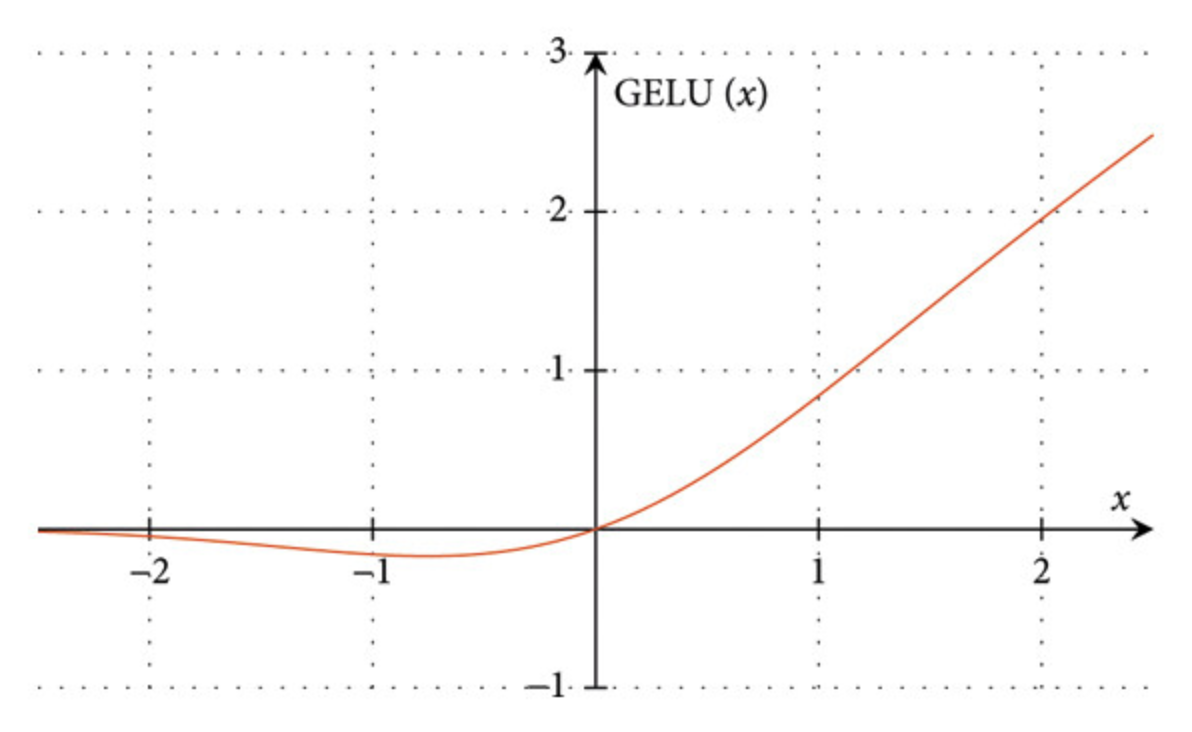
\includegraphics[keepaspectratio]{inserted_images/gelu_graph.png}
\end{center}

We use \href{https://arxiv.org/abs/1606.08415}{GELU} because it is
differentiable everywhere, which helps with calculating gradients during
training, and it has been shown to help Transformer models converge
faster and achieve better performance.

For inputs near zero, GELU acts like a probabilistic gate, outputting
values near zero. For larger inputs, it behaves more like the identity
function (for positives) or suppresses values entirely (for large
negatives). This flexible behavior allows models to learn more nuanced
representations and has been shown to improve performance in
Transformer-based architectures.

Next, we apply a second linear layer with weight matrix \texttt{W\_2} of
shape \texttt{(MLP\_MULT\ ×\ N\_EMBD,\ N\_EMBD)}, producing an output
tensor \texttt{h\_2} of shape \texttt{(TOKEN\_COUNT,\ N\_EMBD)}:

\[
\texttt{h\_2}[t, n] = \sum_{k=1}^{MLP\_MULT \times N\_EMBD} \texttt{h\_1}[t, k] \cdot \texttt{W\_2}[k, n]
\]

Finally, we add a residual connection by summing the MLP output with the
original input:

\[
\texttt{mlp\_activations}[t, n] = \texttt{self\_attention\_activations}[t, n] + \texttt{h\_2}[t, n]
\]

This produces the final output of the MLP block with shape
\texttt{(TOKEN\_COUNT,\ N\_EMBD)}.

\begin{Shaded}
\begin{Highlighting}[]
\CommentTok{\# Algorithm: MLP with GELU Activation and Residual}

\CommentTok{\# Pre{-}MLP normalization}
\NormalTok{self\_attention\_activations\_norm }\OperatorTok{=}\NormalTok{ LayerNorm(self\_attention\_activations)}
\NormalTok{h\_1[t, k] }\OperatorTok{=} \BuiltInTok{sum}\NormalTok{ over n of self\_attention\_activations\_norm[t, n] }\OperatorTok{*}\NormalTok{ W\_1[n, k]}
\NormalTok{h\_1[t, k] }\OperatorTok{=}\NormalTok{ GELU(h\_1[t, k]) }\ControlFlowTok{for} \BuiltInTok{all}\NormalTok{ t, k}
\NormalTok{h\_2[t, n] }\OperatorTok{=} \BuiltInTok{sum}\NormalTok{ over k of h\_1[t, k] }\OperatorTok{*}\NormalTok{ W\_2[k, n]}
\CommentTok{\# Residual connection}
\NormalTok{mlp\_activations[t, n] }\OperatorTok{=}\NormalTok{ self\_attention\_activations\_norm[t, n] }\OperatorTok{+}\NormalTok{ h\_2[t, n]}
\end{Highlighting}
\end{Shaded}

    \subsubsection{Linear Layer}\label{linear-layer}

The linear layer takes in a tensor \texttt{mlp\_activations} of shape
\texttt{(TOKEN\_COUNT,\ N\_EMBD)}.

Before applying the linear transformation, the model applies a final
LayerNorm:

\[
\texttt{mlp\_activations\_norm}[t] = \texttt{LayerNorm}(\texttt{mlp\_activations}[t])
\]

This normalized tensor is then passed through a linear layer with weight
matrix \texttt{W\_vocab} of shape \texttt{(VOCAB\_SIZE,\ N\_EMBD)}.

The linear layer computes logits, which represent unnormalized scores
for each token in the vocabulary. The output tensor has shape
\texttt{(TOKEN\_COUNT,\ VOCAB\_SIZE)}, where each row contains the
logits for predicting the next token at that position in the sequence.

Each output element is computed as:

\[
\texttt{logits}[t, v] = \sum_{n=1}^{N\_EMBD} \texttt{W\_vocab}[v, n] \cdot \texttt{mlp\_activations\_norm}[t, n]
\]

During training, logits for all positions are used. During inference,
only the logits at the final timestep are returned.

\begin{Shaded}
\begin{Highlighting}[]
\CommentTok{\# Algorithm: Linear Layer Transformation}
\NormalTok{mlp\_activations\_norm }\OperatorTok{=}\NormalTok{ LayerNorm(mlp\_activations)     }\CommentTok{\# Final normalization}
\NormalTok{logits[t, v] }\OperatorTok{=} \BuiltInTok{sum}\NormalTok{ over n of mlp\_activations\_norm[t, n] }\OperatorTok{*}\NormalTok{ W\_vocab[v, n]}
\ControlFlowTok{if}\NormalTok{ training:}
    \ControlFlowTok{return}\NormalTok{ logits                                     }\CommentTok{\# shape (TOKEN\_COUNT, VOCAB\_SIZE)}
\ControlFlowTok{else}\NormalTok{:}
    \ControlFlowTok{return}\NormalTok{ logits[}\OperatorTok{{-}}\DecValTok{1}\NormalTok{]                                 }\CommentTok{\# shape (VOCAB\_SIZE,)}
\end{Highlighting}
\end{Shaded}

    \subsubsection{Generator}\label{generator}

The generator function takes as input a sequence \texttt{seq} of shape
\texttt{(TOKEN\_COUNT)} and a target number \texttt{M} indicating how
many new tokens to generate. It iteratively appends tokens to the
sequence by performing a forward pass and sampling the next token from
the model's output.

The process is repeated for \texttt{M} steps. In each step, the sequence
is trimmed if necessary to ensure that its length does not exceed the
model's \texttt{block\_size}. A forward pass through the model produces
logits, which are converted to probabilities using softmax. A new token
is then sampled from this distribution and appended to the sequence.

\begin{Shaded}
\begin{Highlighting}[]
\CommentTok{\# Algorithm: Generator – Token Generation}
\ControlFlowTok{for}\NormalTok{ step }\KeywordTok{in} \BuiltInTok{range}\NormalTok{(M):}
\NormalTok{    trimmed\_seq }\OperatorTok{=}\NormalTok{ seq[}\OperatorTok{{-}}\NormalTok{BLOCK\_SIZE:]     }\CommentTok{\# Trim sequence if needed}
\NormalTok{    logits }\OperatorTok{=}\NormalTok{ model(trimmed\_seq)         }\CommentTok{\# Forward pass → shape (TOKEN\_COUNT, VOCAB\_SIZE)}
\NormalTok{    last\_logits }\OperatorTok{=}\NormalTok{ logits[}\OperatorTok{{-}}\DecValTok{1}\NormalTok{]            }\CommentTok{\# Take logits at last timestep → shape (VOCAB\_SIZE,)}
\NormalTok{    probs }\OperatorTok{=}\NormalTok{ softmax(last\_logits)        }\CommentTok{\# Convert to probabilities}
\NormalTok{    new\_token }\OperatorTok{=}\NormalTok{ sample\_from(probs)      }\CommentTok{\# Sample next token}
\NormalTok{    seq }\OperatorTok{=}\NormalTok{ append(seq, new\_token)        }\CommentTok{\# Add token to sequence}
\ControlFlowTok{return}\NormalTok{ seq                              }\CommentTok{\# Final sequence after M steps}
\end{Highlighting}
\end{Shaded}

    \subsubsection{Full Steps from Input to
Output}\label{full-steps-from-input-to-output}

Here, we show a diagram and summarize the entire sequence from input to
output:

\begin{center}
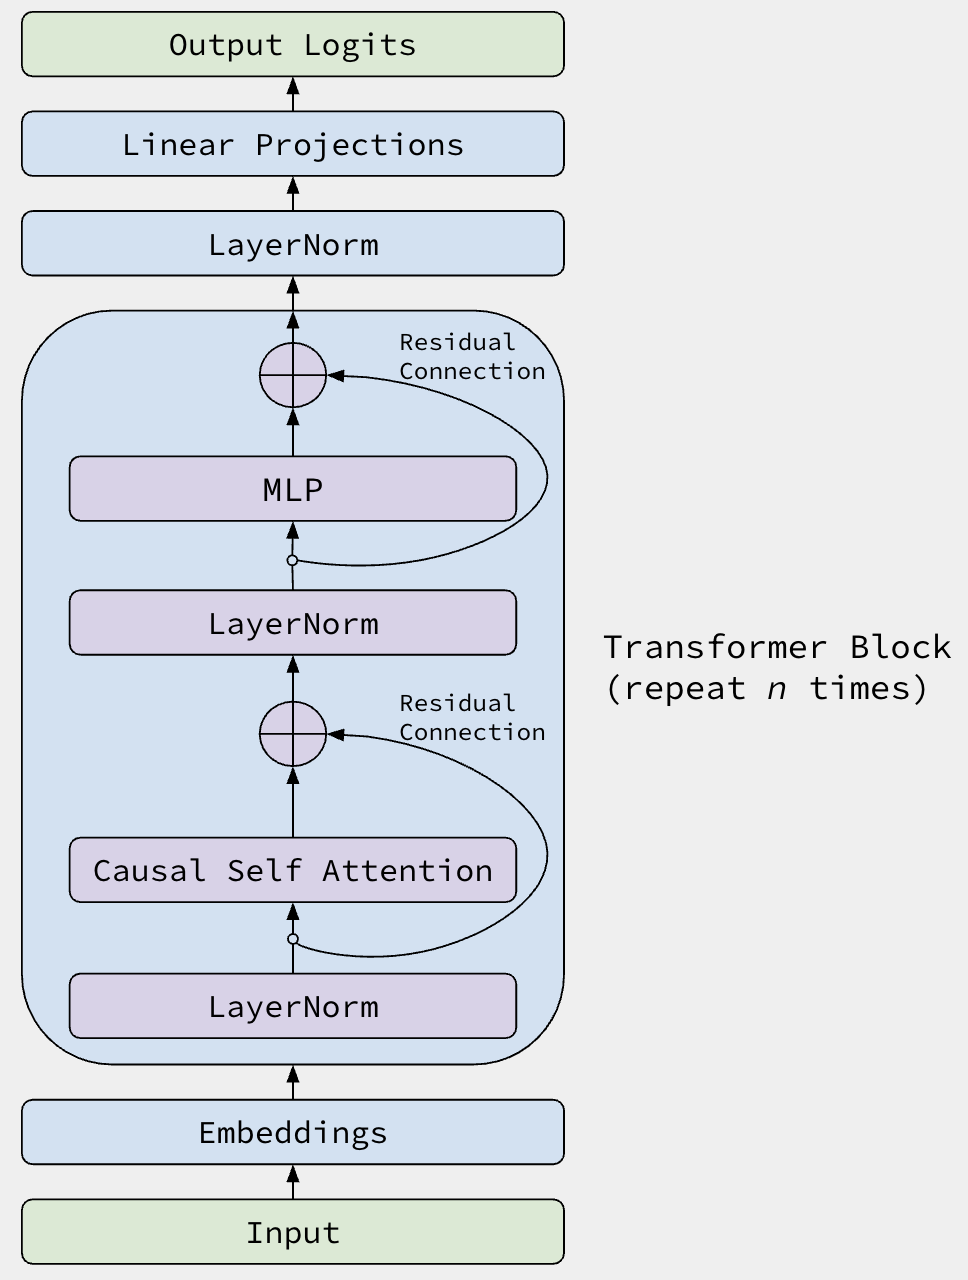
\includegraphics[width=0.6\textwidth, keepaspectratio]{inserted_images/model_arch.png}
\end{center}

\begin{Shaded}
\begin{Highlighting}[]
\CommentTok{\# Step 1: Input}
\CommentTok{\# Input: tensor x of shape (TOKEN\_COUNT)}
\NormalTok{x }\OperatorTok{=}\NormalTok{ input\_tensor}

\CommentTok{\# Step 2: Embeddings}
\NormalTok{tok\_emb }\OperatorTok{=}\NormalTok{ TokenEmbedding(x, W\_e)           }\CommentTok{\# Token embeddings → shape (TOKEN\_COUNT, N\_EMBD)}
\NormalTok{pos\_emb }\OperatorTok{=}\NormalTok{ PositionEmbedding(T, W\_p)        }\CommentTok{\# Position embeddings → shape (TOKEN\_COUNT, N\_EMBD)}
\NormalTok{emb }\OperatorTok{=}\NormalTok{ tok\_emb }\OperatorTok{+}\NormalTok{ pos\_emb                    }\CommentTok{\# Combined embeddings → shape (TOKEN\_COUNT, N\_EMBD)}
\NormalTok{activations }\OperatorTok{=}\NormalTok{ emb}
\CommentTok{\# Step 3: Apply Transformer Blocks}
\ControlFlowTok{for}\NormalTok{ layer }\KeywordTok{in} \BuiltInTok{range}\NormalTok{(LAYER\_COUNT):}

    \CommentTok{\# LayerNorm + Self{-}Attention}
\NormalTok{    activations\_norm }\OperatorTok{=}\NormalTok{ LayerNorm(activations)}
\NormalTok{    residual }\OperatorTok{=}\NormalTok{ activations\_norm               }\CommentTok{\# Store input for the residual connection}
\NormalTok{    qkv }\OperatorTok{=}\NormalTok{ activations\_norm }\OperatorTok{@}\NormalTok{ W\_qkv            }\CommentTok{\# Project to Q, K, V → (TOKEN\_COUNT, 3 × N\_EMBD)}
\NormalTok{    q, k, v }\OperatorTok{=}\NormalTok{ split(qkv)                      }\CommentTok{\# (TOKEN\_COUNT, N\_EMBD) each}
\NormalTok{    q, k, v }\OperatorTok{=}\NormalTok{ transpose\_heads(q, k, v)        }\CommentTok{\# (HEAD\_COUNT, TOKEN\_COUNT, DIM\_PER\_HEAD)}
\NormalTok{    attn\_weight }\OperatorTok{=}\NormalTok{ dot(q, k) }\OperatorTok{+}\NormalTok{ attn\_bias       }\CommentTok{\# (HEAD\_COUNT, TOKEN\_COUNT, TOKEN\_COUNT)}
\NormalTok{    attn\_weight }\OperatorTok{=}\NormalTok{ softmax(attn\_weight)}
\NormalTok{    attn\_output }\OperatorTok{=}\NormalTok{ weighted\_sum(attn\_weight, v)     }\CommentTok{\# (HEAD\_COUNT, TOKEN\_COUNT, DIM\_PER\_HEAD)}
\NormalTok{    attn\_output }\OperatorTok{=}\NormalTok{ merge\_heads(attn\_output)         }\CommentTok{\# (TOKEN\_COUNT, N\_EMBD)}
\NormalTok{    attn\_proj }\OperatorTok{=}\NormalTok{ attn\_output }\OperatorTok{@}\NormalTok{ W\_c\_proj             }\CommentTok{\# Output projection}
\NormalTok{    activations }\OperatorTok{=}\NormalTok{ residual }\OperatorTok{+}\NormalTok{ attn\_proj             }\CommentTok{\# Residual connection}

    \CommentTok{\# LayerNorm + MLP}
\NormalTok{    self\_attention\_activations }\OperatorTok{=}\NormalTok{ activations}
\NormalTok{    residual }\OperatorTok{=}\NormalTok{ self\_attention\_activations       }\CommentTok{\# Store input for the residual connection}
\NormalTok{    self\_attention\_activations\_norm }\OperatorTok{=}\NormalTok{ LayerNorm(self\_attention\_activations)}
\NormalTok{    h\_1 }\OperatorTok{=}\NormalTok{ self\_attention\_activations\_norm }\OperatorTok{@}\NormalTok{ W\_1  }
                                        \CommentTok{\# First linear → (TOKEN\_COUNT, MLP\_MULT × N\_EMBD)}
\NormalTok{    h\_1 }\OperatorTok{=}\NormalTok{ GELU(h\_1)                              }\CommentTok{\# Activation}
\NormalTok{    h\_2 }\OperatorTok{=}\NormalTok{ h\_1 }\OperatorTok{@}\NormalTok{ W\_2                              }\CommentTok{\# Second linear → (TOKEN\_COUNT, N\_EMBD)}
\NormalTok{    mlp\_activations }\OperatorTok{=}\NormalTok{ residual }\OperatorTok{+}\NormalTok{ h\_2             }\CommentTok{\# Residual connection}

\CommentTok{\# Step 4: Final LayerNorm}
\NormalTok{mlp\_activations\_norm }\OperatorTok{=}\NormalTok{ LayerNorm(mlp\_activations)       }\CommentTok{\# (TOKEN\_COUNT, N\_EMBD)}

\CommentTok{\# Step 5: Output projection (to vocabulary)}
\NormalTok{logits }\OperatorTok{=}\NormalTok{ mlp\_activations\_norm }\OperatorTok{@}\NormalTok{ W\_vocab                 }\CommentTok{\# shape (TOKEN\_COUNT, VOCAB\_SIZE)}
\end{Highlighting}
\end{Shaded}

    \subsection{Parameter Allocation
Experiments}\label{parameter-allocation-experiments}

As discussed earlier, we initialize a GPT model by specifying the number
of attention heads, transformer blocks, and the embedding dimension.
Increasing the number of transformer blocks (\texttt{n\_layer}) and the
size of the embedding dimension (\texttt{n\_embd}) increases the total
number of parameters in the model. This introduces a tradeoff: larger
models tend to be more capable, but they also take longer to train.

We were interested in understanding the best way to allocate a fixed
budget of parameters. In other words, if we can afford a model with
roughly \emph{n} parameters, how should we distribute those parameters
across layers and embedding dimensions to get the best performance?

To explore this, we compared models with
\texttt{n\_layer\ =\ 1,\ 2,\ 3,\ or\ 4} transformer blocks. For each
model, we adjusted the embedding dimension so that the total parameter
count remained similar. All models used a single attention head
(\texttt{n\_head\ =\ 1}) for consistency. The table below shows the
architectures we tested:

\begin{longtable}[]{@{}lll@{}}
\toprule\noalign{}
\texttt{n\_layer} & \texttt{n\_embd} & Total Parameters \\
\midrule\noalign{}
\endhead
\bottomrule\noalign{}
\endlastfoot
1 & 24 & 7,248 \\
2 & 17 & 7,208 \\
3 & 14 & 7,308 \\
4 & 12 & 7,152 \\
\end{longtable}

For reference, the original minimal model used throughout this report
has \texttt{n\_layer\ =\ 1}, \texttt{n\_embd\ =\ 12}, and 1,896
parameters, so all of these architectures are substantially larger and
more complex.

We conducted 15 training trials for each architecture, training for
100,000 iterations per run. Below are the average training curves:

\begin{center}
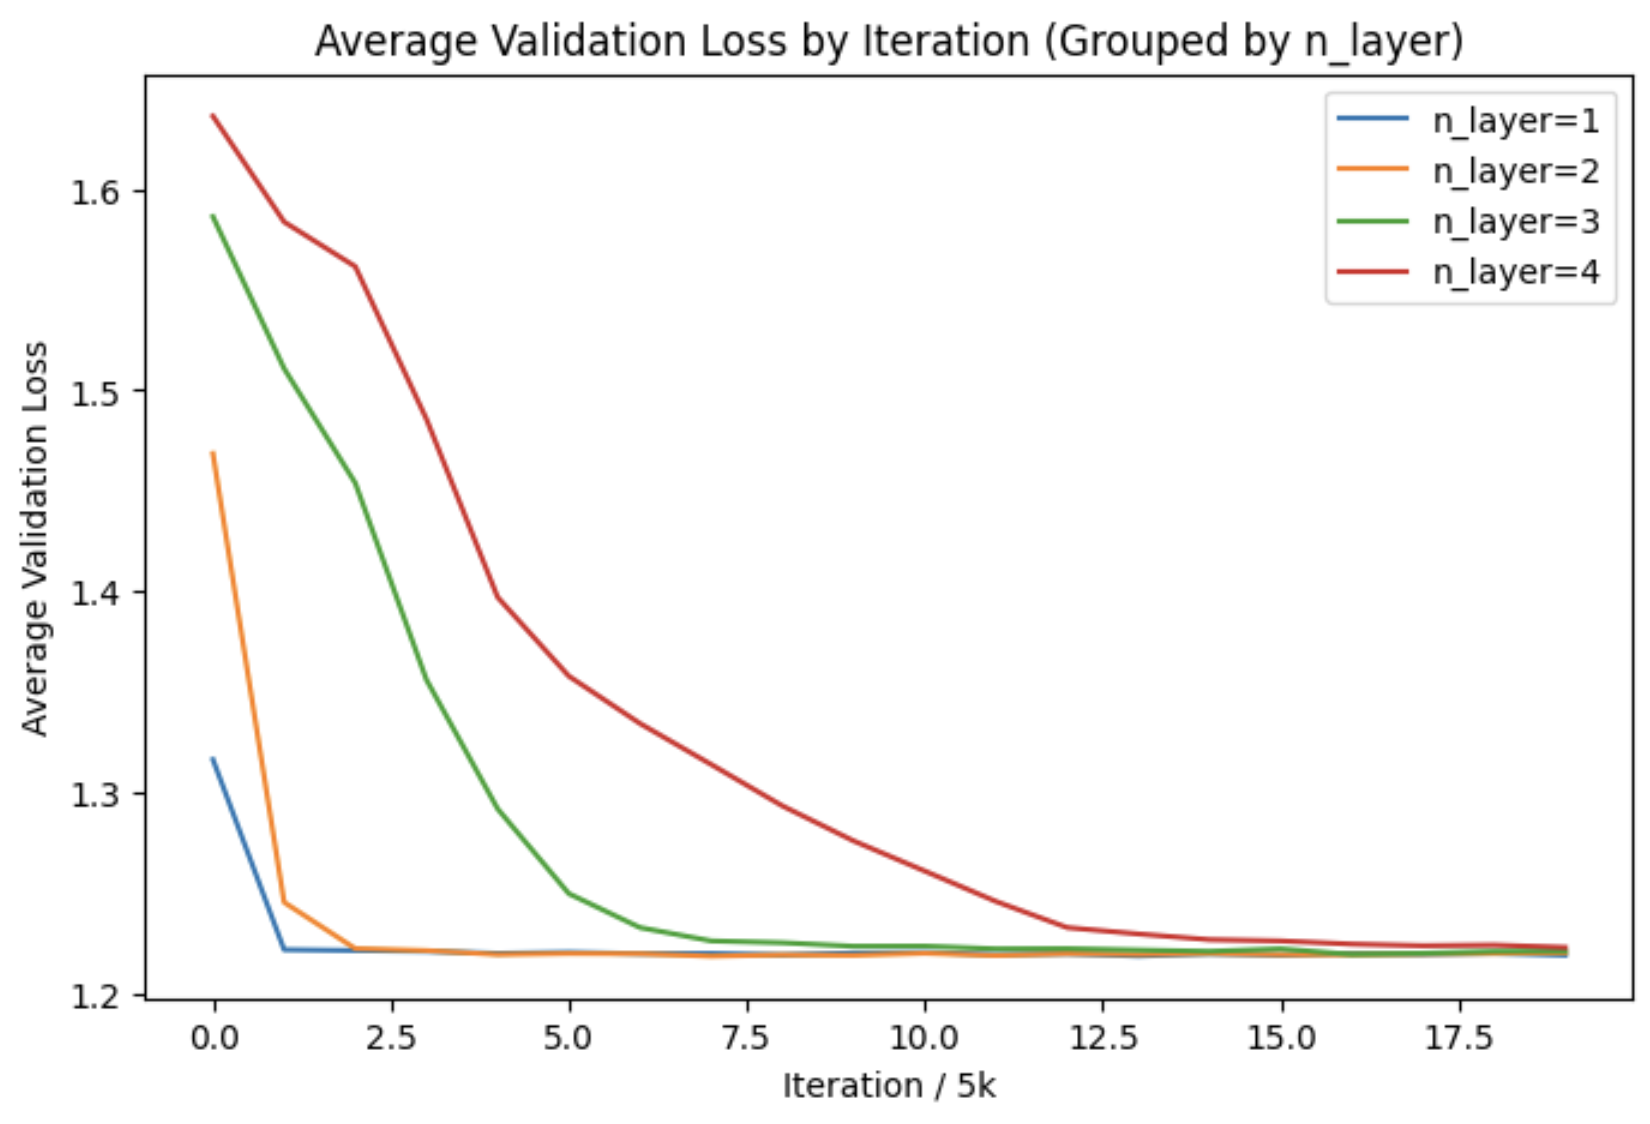
\includegraphics[keepaspectratio]{inserted_images/diff_layer_runs.png}
\end{center}

What can we conclude from this experiment? Honestly, not much. All of
these models are more powerful than the minimal configuration we already
knew could learn the task, so it's not surprising that they all
succeeded. And, because adding more transformer blocks increases the
depth of the function the model needs to learn, it's also unsurprising
that deeper models converged more slowly. This experiment might be more
informative in the context of a harder task where models are not all
guaranteed to succeed, and where differences in generalization or
learning speed could be more meaningful. In that setting, parameter
allocation might have a clearer impact on final performance.

    \subsection{Probing a Multi-Headed
Model}\label{probing-a-multi-headed-model}

\subsubsection{Motivation}\label{motivation}

We previously identified two core rules of tic-tac-toe and observed that
a single-headed model often learned them in two distinct phases. This
led us to wonder what would happen if we give the model a second
attention head? Could each head specialize in a different rule,
eliminating the staggered learning pattern?

To explore this, we trained a model with \texttt{n\_layer\ =\ 1},
\texttt{n\_head\ =\ 2}, and \texttt{n\_embd\ =\ 12}, a setup which
yielded the same number of parameters as the original, one-headed model.
We ran 20 training trials, training for 100,000 iterations, and 80\% of
runs converged. Take a look at all of the converging two-headed training
runs below:

\begin{center}
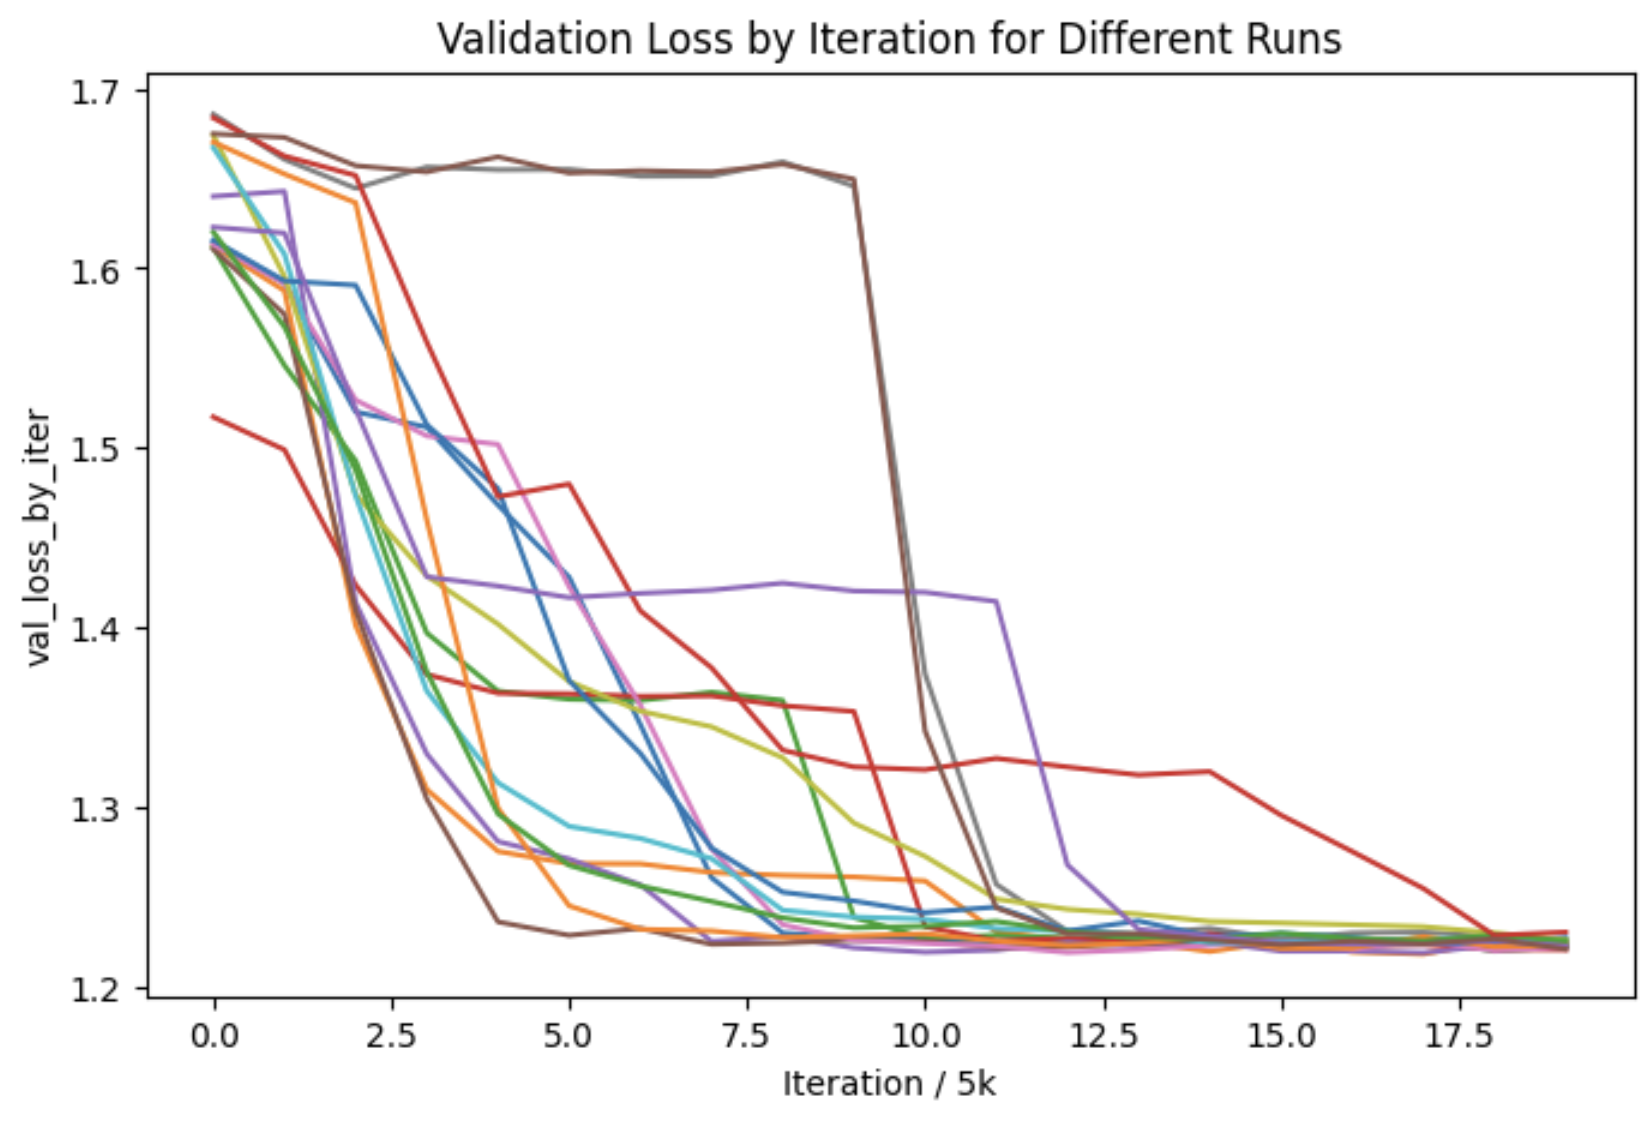
\includegraphics[keepaspectratio]{inserted_images/converging_2_heads.png}
\end{center}

Overall, there seems to be less of a pattern in this training than there
was when we trained the original model. Only one of these training
trials stalled with a validation loss between 1.36 and 1.37, where we
saw stalling occur before, and there does not seem to be a new
consistent place where training does stall. In contrast, many of the
training runs look relatively smooth and converge quickly.

    \subsubsection{Setup}\label{setup}

Based on these trends, we suspected that the two-headed model might be
training in a fundamentally different way. The training run we took data
from seemed typical for this new architecture and is shown below,:

\begin{center}
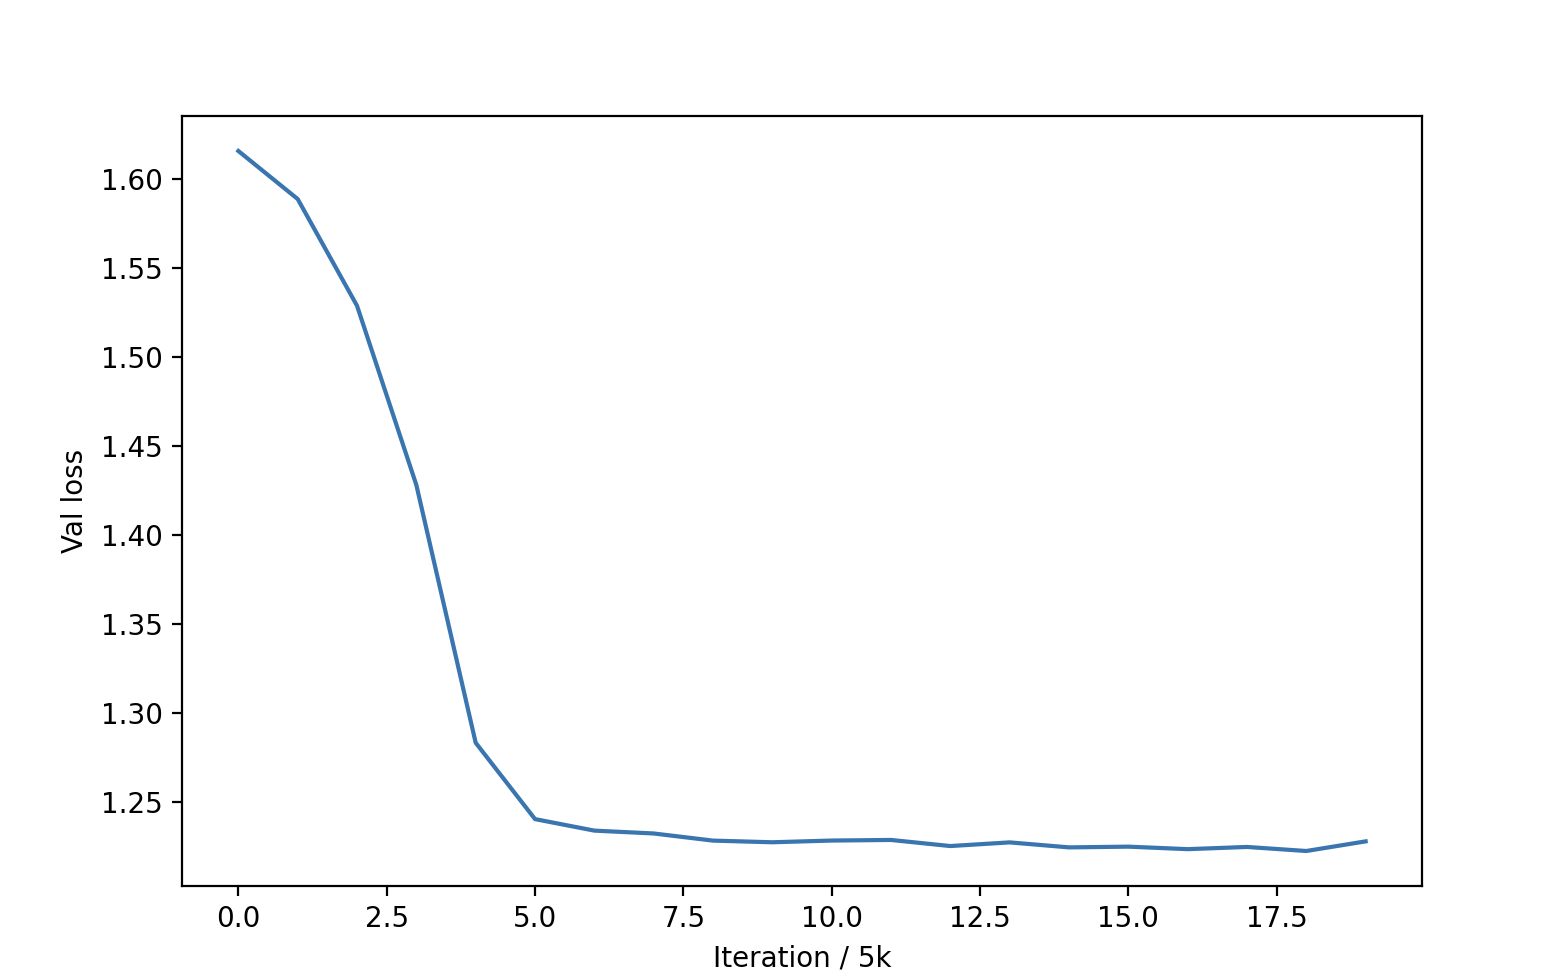
\includegraphics[keepaspectratio]{inserted_images/probing_trial_2h.png}
\end{center}

We saved checkpoints at the same stages as with the one-headed model:

\begin{itemize}
\tightlist
\item
  Random start
\item
  After loss dropped below 1.37 (``Stalling Begins'' checkpoint)
\item
  After loss dropped below 1.36 (``Stalling Ends'' checkpoint)
\item
  Fully trained
\end{itemize}

We then followed the same probing procedure, training three probes
(Linear, Small MLP, and Large MLP) to use the model's activations to
predict the Space Occupancy and Win Detection tasks. If our hypothesis
was true and each head did learn a different rule, what might we expect?
We thought we might notice the following:

\begin{enumerate}
\def\labelenumi{\arabic{enumi}.}
\item
  \textbf{No fundamental change between Stalling Begins and Stalling
  Ends checkpoints}\\
  In the one-headed model, the transition between these checkpoints came
  with a large change in probe performance as the model started to learn
  to detect a winner. However, if each head now learns its rule
  independently, we wouldn't expect such a major shift in internal
  representation, especially at the same place where it happened
  originally.
\item
  \textbf{Space Occupancy and Win Detection being learned together.}\\
  With shared responsibility, both tasks should improve at the same time
  throughout training. We're not expecting a staged progression where
  one rule is represented before another anymore, but rather steady
  improvement as the model gets better overall.
\item
  \textbf{Head-level specialization in probe results.}\\
  If heads divide up the rules, then probing individual head outputs
  should show one head consistently better at Space Occupancy and the
  other at Win Detection, corresponding to the rules they represent.
\end{enumerate}

    \subsubsection{Full Model Probing}\label{full-model-probing}

We first explore how the model's representations evolve across
checkpoints, hoping to answer our first two questions. Probes were
trained on activations taken after the final LayerNorm, using the same
setup as in the one-headed case. Results are shown in both table and
graphical form below:

\paragraph{Linear Probe}\label{linear-probe}

\begin{longtable}[]{@{}
  >{\raggedright\arraybackslash}p{(\linewidth - 8\tabcolsep) * \real{0.2368}}
  >{\raggedright\arraybackslash}p{(\linewidth - 8\tabcolsep) * \real{0.1053}}
  >{\raggedright\arraybackslash}p{(\linewidth - 8\tabcolsep) * \real{0.2368}}
  >{\raggedright\arraybackslash}p{(\linewidth - 8\tabcolsep) * \real{0.2105}}
  >{\raggedright\arraybackslash}p{(\linewidth - 8\tabcolsep) * \real{0.2105}}@{}}
\toprule\noalign{}
\begin{minipage}[b]{\linewidth}\raggedright
Task
\end{minipage} & \begin{minipage}[b]{\linewidth}\raggedright
Random
\end{minipage} & \begin{minipage}[b]{\linewidth}\raggedright
Stalling Begins
\end{minipage} & \begin{minipage}[b]{\linewidth}\raggedright
Stalling Ends
\end{minipage} & \begin{minipage}[b]{\linewidth}\raggedright
Fully Trained
\end{minipage} \\
\midrule\noalign{}
\endhead
\bottomrule\noalign{}
\endlastfoot
Space Occupancy & 0.658 & 0.909 & 0.907 & 0.954 \\
Win Detection & 0.905 & 0.966 & 0.966 & 0.969 \\
\end{longtable}

\paragraph{Small MLP Probe}\label{small-mlp-probe}

\begin{longtable}[]{@{}
  >{\raggedright\arraybackslash}p{(\linewidth - 8\tabcolsep) * \real{0.2368}}
  >{\raggedright\arraybackslash}p{(\linewidth - 8\tabcolsep) * \real{0.1053}}
  >{\raggedright\arraybackslash}p{(\linewidth - 8\tabcolsep) * \real{0.2368}}
  >{\raggedright\arraybackslash}p{(\linewidth - 8\tabcolsep) * \real{0.2105}}
  >{\raggedright\arraybackslash}p{(\linewidth - 8\tabcolsep) * \real{0.2105}}@{}}
\toprule\noalign{}
\begin{minipage}[b]{\linewidth}\raggedright
Task
\end{minipage} & \begin{minipage}[b]{\linewidth}\raggedright
Random
\end{minipage} & \begin{minipage}[b]{\linewidth}\raggedright
Stalling Begins
\end{minipage} & \begin{minipage}[b]{\linewidth}\raggedright
Stalling Ends
\end{minipage} & \begin{minipage}[b]{\linewidth}\raggedright
Fully Trained
\end{minipage} \\
\midrule\noalign{}
\endhead
\bottomrule\noalign{}
\endlastfoot
Space Occupancy & 0.790 & 0.954 & 0.954 & 0.972 \\
Win Detection & 0.925 & 0.988 & 0.988 & 0.988 \\
\end{longtable}

\paragraph{Large MLP Probe}\label{large-mlp-probe}

\begin{longtable}[]{@{}
  >{\raggedright\arraybackslash}p{(\linewidth - 8\tabcolsep) * \real{0.2368}}
  >{\raggedright\arraybackslash}p{(\linewidth - 8\tabcolsep) * \real{0.1053}}
  >{\raggedright\arraybackslash}p{(\linewidth - 8\tabcolsep) * \real{0.2368}}
  >{\raggedright\arraybackslash}p{(\linewidth - 8\tabcolsep) * \real{0.2105}}
  >{\raggedright\arraybackslash}p{(\linewidth - 8\tabcolsep) * \real{0.2105}}@{}}
\toprule\noalign{}
\begin{minipage}[b]{\linewidth}\raggedright
Task
\end{minipage} & \begin{minipage}[b]{\linewidth}\raggedright
Random
\end{minipage} & \begin{minipage}[b]{\linewidth}\raggedright
Stalling Begins
\end{minipage} & \begin{minipage}[b]{\linewidth}\raggedright
Stalling Ends
\end{minipage} & \begin{minipage}[b]{\linewidth}\raggedright
Fully Trained
\end{minipage} \\
\midrule\noalign{}
\endhead
\bottomrule\noalign{}
\endlastfoot
Space Occupancy & 0.837 & 0.977 & 0.977 & 0.980 \\
Win Detection & 0.925 & 0.989 & 0.990 & 0.990 \\
\end{longtable}

\paragraph{Results Plotted}\label{results-plotted}

\vspace{1em}

\begin{center}
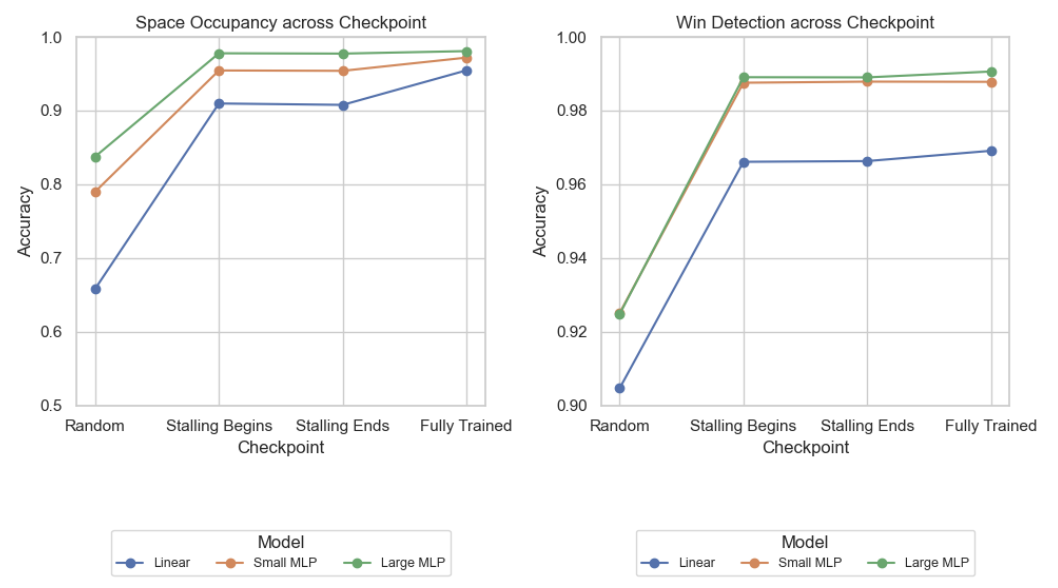
\includegraphics[width=\textwidth, keepaspectratio]{inserted_images/two_head_by_ckpt.png}
\end{center}
At the final checkpoint, probe performance is comparable to that seen
with the original one-headed model. This suggests that architectural
changes didn't affect the model's capacity to form accurate internal
representations.

The loss curve gave no indication of a major shift between the second
and third checkpoints, and the probe results confirm this intuition. For
all probe types and tasks, probe performances at these checkpoints are
nearly identical.

Both tasks are learned well, though Win Detection appears to be picked
up slightly earlier. Still, Space Occupancy continues to improve
steadily through to the end of training. This suggests that both
internal representations are learned simultaneously, albeit at slightly
different rates.

    \subsubsection{Probing Individual Heads}\label{probing-individual-heads}

We also captured activations from inside the transformer block before
the outputs of the two attention heads were combined, and separated
these activations into those coming from Head 0 and Head 1. If each head
were learning a distinct rule, we'd expect a clear pattern of
specialization: probes trained on Head 0's activations would perform
well on one task, and probes on Head 1's activations would perform well
on the other. The results of this experiment are shown below:

\begin{center}
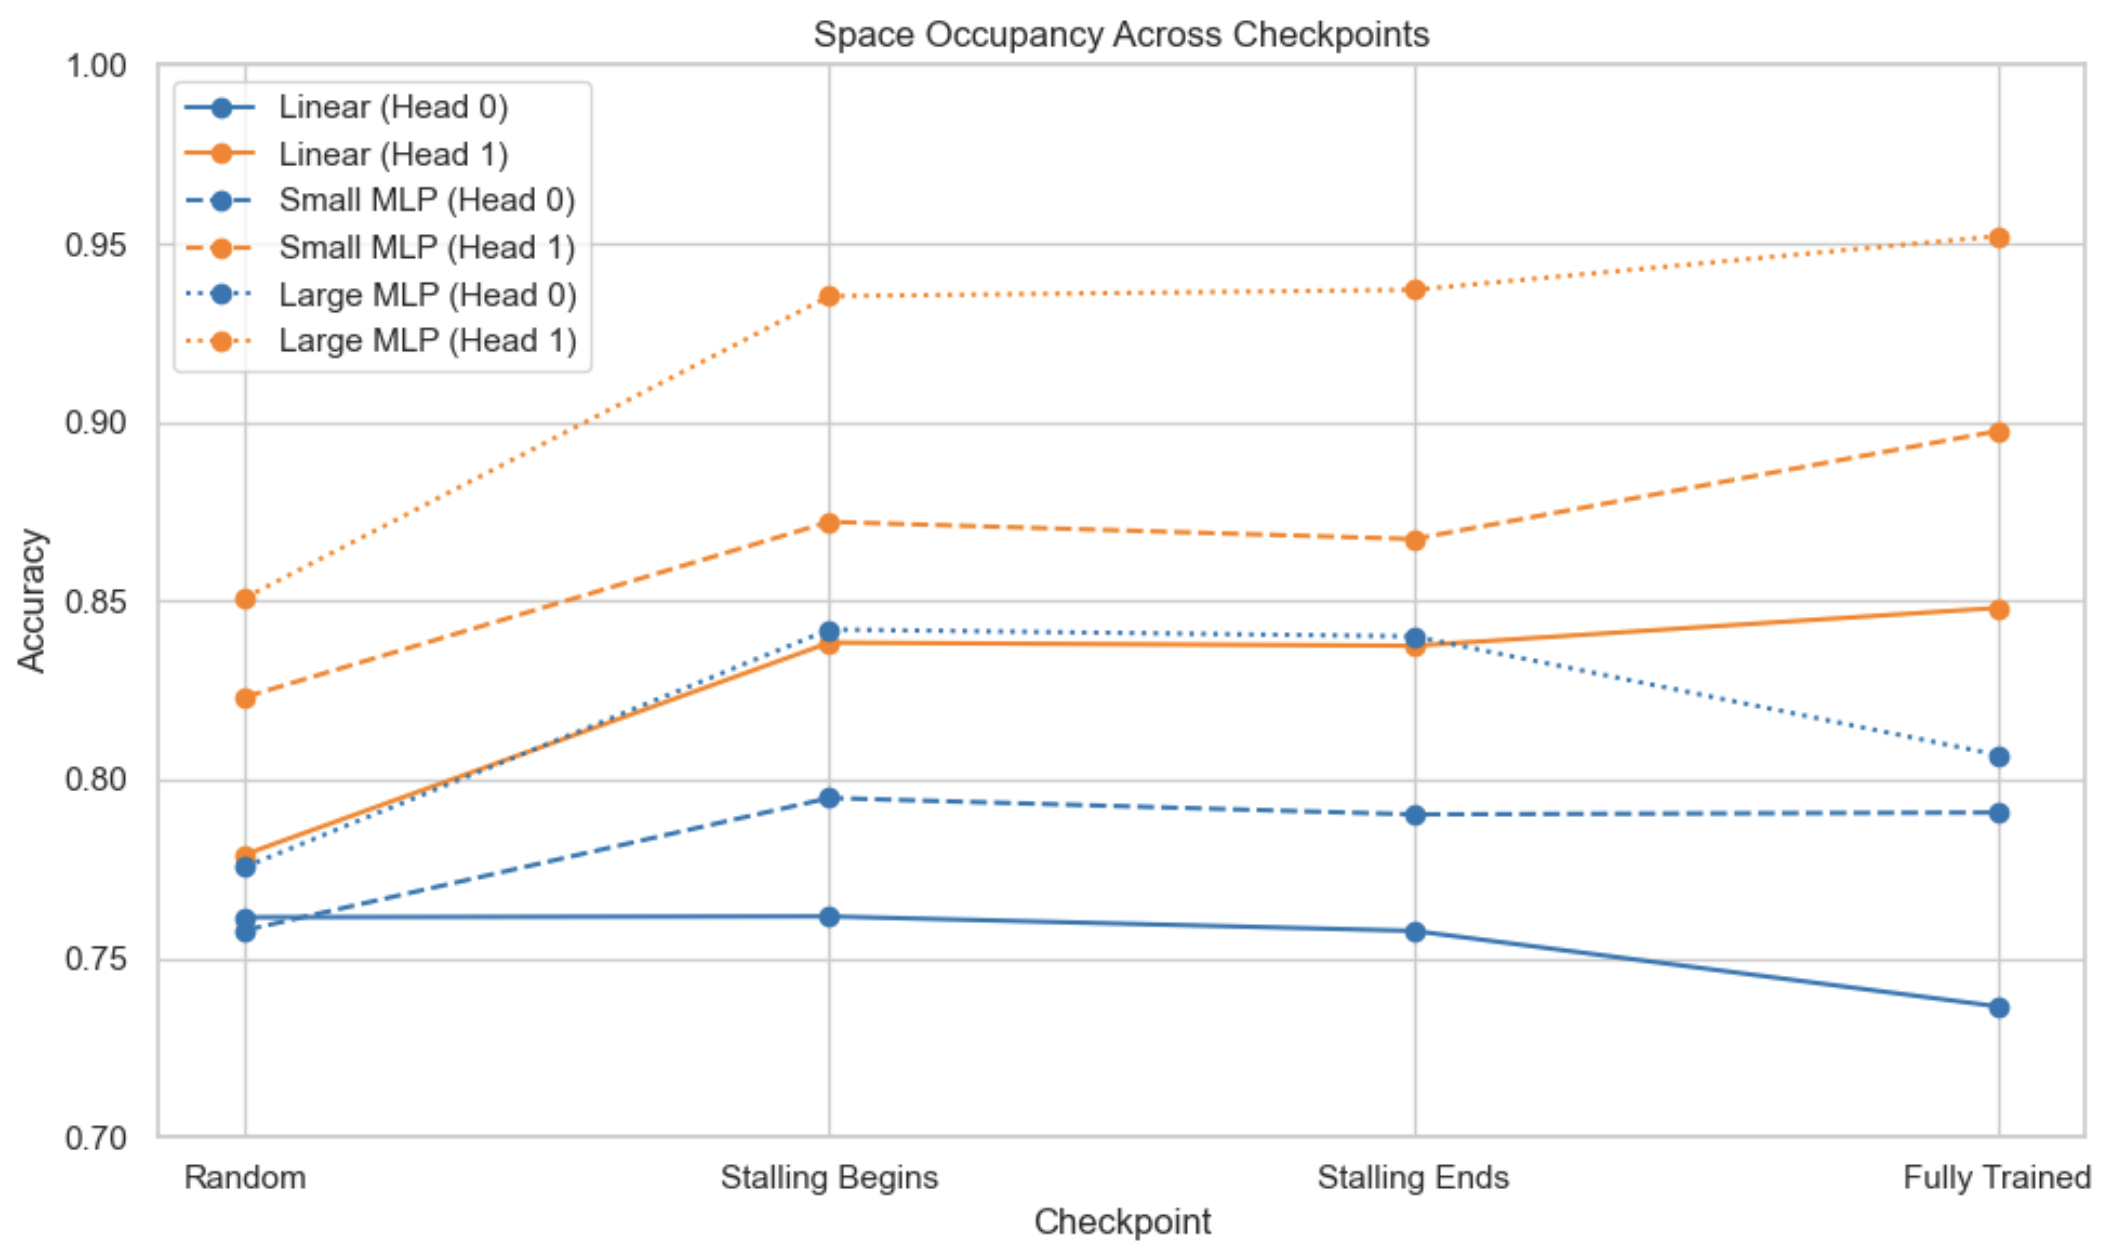
\includegraphics[keepaspectratio]{inserted_images/so_two_head.png}
\end{center}

\begin{center}
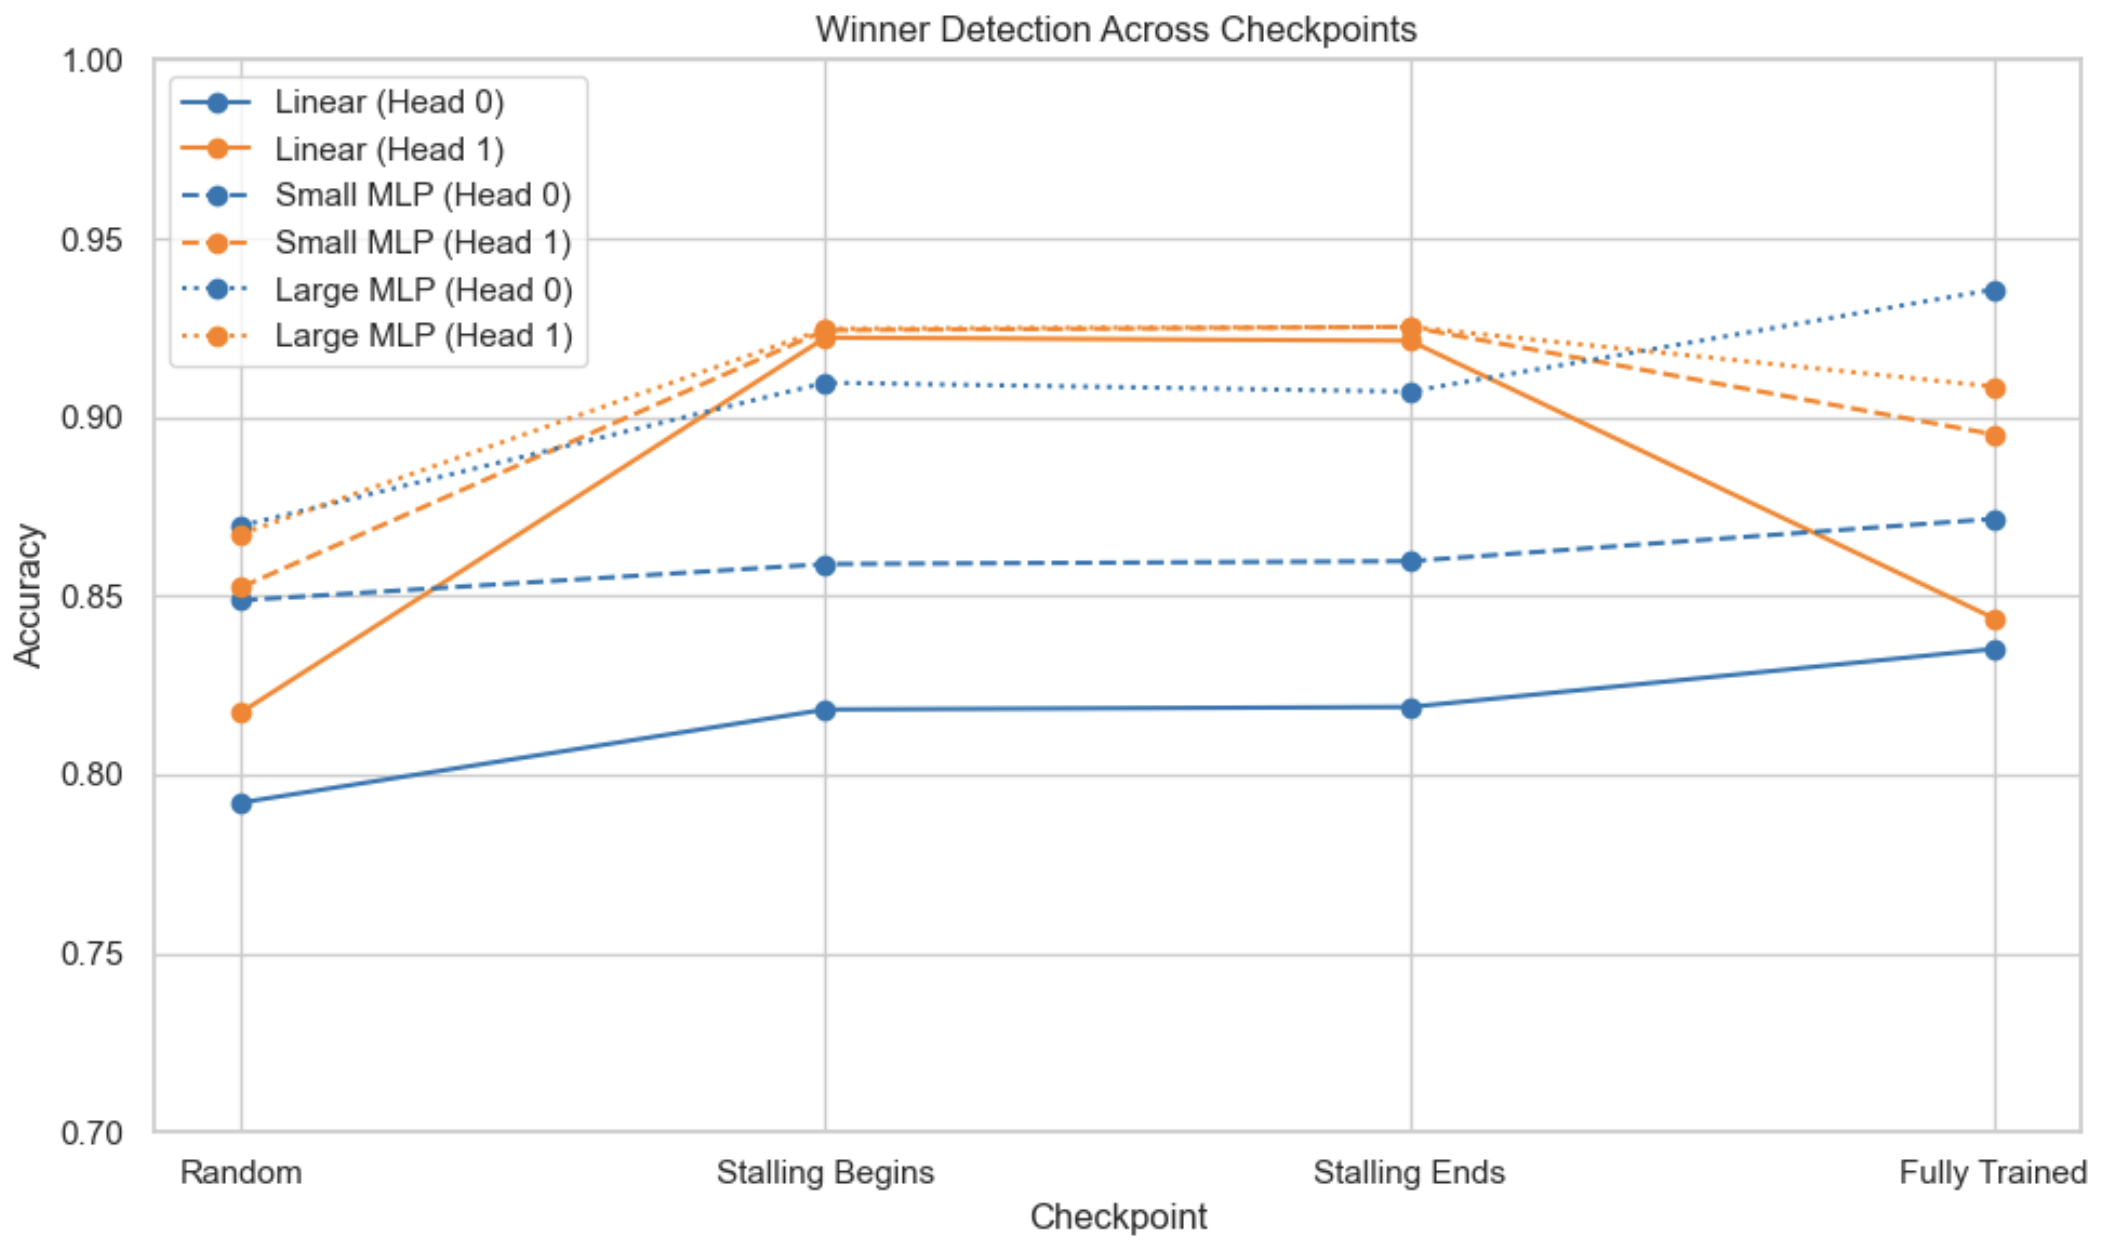
\includegraphics[keepaspectratio]{inserted_images/wd_two_head.png}
\end{center}

As expected, these probe accuracies are lower than those trained on full
activations. This is because when we isolate a single head from a
two-headed model, we remove half of the activations the model would
otherwise use.

For Space Occupancy, probes trained on Head 1's activations consistently
outperform those trained on Head 0's, across all checkpoints, including
the randomly initialized one. This early gap might be due to lucky
initialization, but it holds throughout training. By the end, the Head 1
probe reaches high accuracy, suggesting that Head 1 plays a dominant
role in representing this rule.

Win Detection shows less clear contrast between probes. Between the
Stalling Begins and Stalling Ends checkpoints, probes trained on Head
1's activations perform better than those from Head 0, suggesting it
initially captures this structure more effectively as well. By the Fully
Trained checkpoint, however, Head 1's probe performance actually
declines, and both heads yield similar results. This suggests that Win
Detection representation is done with both heads contributing, rather
than with one head specializing.

    \subsubsection{Takeaways}\label{takeaways}

The two-headed model clearly learns differently from the one-headed
version. Both Space Occupancy and Win Detection are learned
simultaneously with no major shift between the Stalling Begins and
Stalling Ends checkpoints. There's steady improvement on both tasks
throughout training, not a pattern where one task is learned completely
before learning on the other starts.

We do see some signs of specialization: Probes trained Head 1 handle the
Space Occupancy much better than probes trained on Head 0. For Win
Detection, though, both heads contribute, and neither clearly dominates.
We also observe a strange pattern where probes trained on Head 1 are
strong at this task early in training, but get weaker by the time
training ends.

We couldn't fully identify the roles of each head or state definitively
how the two-headed model trains, as the results we observe are
unintuitive, and very interesting. This could definitely be a path for
future research, but I unfortunately ran out of time before my thesis
was due.

\begin{thebibliography}{99}

\bibitem{alain2016understanding}
Guillaume Alain and Yoshua Bengio.
\newblock Understanding intermediate layers using linear classifier probes.
\newblock \emph{arXiv preprint arXiv:1610.01644}, 2016.
\newblock \url{https://arxiv.org/abs/1610.01644}.

\bibitem{haeusler2023tic}
Phillip Haeusler.
\newblock Tic Tac Transformer.
\newblock Personal website, 2023.
\newblock \url{https://philliphaeusler.com/posts/tic_tac_toe/}.

\bibitem{hendrycks2016gelu}
Dan Hendrycks and Kevin Gimpel.
\newblock Gaussian Error Linear Units (GELUs).
\newblock \emph{arXiv preprint arXiv:1606.08415}, 2016.
\newblock \url{https://arxiv.org/abs/1606.08415}.

\bibitem{hsu2020mnk}
Wei-Yuan Hsu, Chu-Ling Ko, Jr-Chang Chen, Ting-Han Wei, Chu-Hsuan Hsueh, and I-Chen Wu.
\newblock On solving the 7,7,5-game and the 8,8,5-game.
\newblock \emph{Theoretical Computer Science}, 816:75--90, 2020.
\newblock \url{https://doi.org/10.1016/j.tcs.2020.02.023}.

\bibitem{karpathy2023gpt}
Andrej Karpathy.
\newblock Let's build GPT: from scratch, in code, spelled out.
\newblock YouTube, 2023.
\newblock \url{https://www.youtube.com/watch?v=kCc8FmEb1nY}.

\bibitem{lee2023gelu}
Minhyeok Lee.
\newblock Mathematical Analysis and Performance Evaluation of the GELU Activation Function in Deep Learning.
\newblock \emph{Mathematical Problems in Engineering}, 2023.
\newblock \url{https://onlinelibrary.wiley.com/doi/10.1155/2023/4229924}.

\bibitem{li2022emergent}
Kenneth Li, Aspen K. Hopkins, David Bau, Fernanda Viégas, Hanspeter Pfister, and Martin Wattenberg.
\newblock Emergent World Representations: Exploring a Sequence Model Trained on a Synthetic Task.
\newblock \emph{arXiv preprint arXiv:2210.13382}, 2022.
\newblock \url{https://arxiv.org/abs/2210.13382}.

\bibitem{nanda2023othello}
Neel Nanda.
\newblock Actually, Othello-GPT Has A Linear Emergent World Representation.
\newblock Blog post, 2023.
\newblock \url{https://www.neelnanda.io/mechanistic-interpretability/othello}.

\bibitem{vaswani2017attention}
Ashish Vaswani et al.
\newblock Attention Is All You Need.
\newblock \emph{Advances in Neural Information Processing Systems}, 30, 2017.
\newblock \url{https://arxiv.org/abs/1706.03762}.

\end{thebibliography}
    
\end{document}
